\documentclass[whitelogo]{tudelft-report}
\usepackage{multirow}
\usepackage{natbib}
\usepackage{changes}
%\usepackage[demo]{graphicx}
%\usepackage{caption}
\usepackage{subcaption}
\usepackage[section]{placeins}
\geometry{
	a4paper,
	total={160mm,252mm},
	left=25mm,
	top=25mm,
}
%\usepackage[table,xcdraw]{xcolor}
\usepackage{titlesec}
\usepackage[section]{placeins}
\usepackage[
    %backend=biber, 
    natbib=true,
    style=numeric,
    sorting=none
]% {biblatex}
%\addbibresource{report.bib}
% \usepackage[backend=biber,style=numeric,sorting=none]{biblatex}
\usepackage{float}





% \usepackage[table,xcdraw]{xcolor}
% %\usepackage{titlesec}
% \usepackage{cite}
% \usepackage{tikz}

\usepackage{amsmath}
\usepackage{enumerate}
\usepackage{graphicx}
\usepackage{epstopdf}
\usepackage{a4wide,times}
\usepackage{listings}
\usepackage{lastpage}
\usepackage{fancy hdr}
%\usepackage{placeins}
\usepackage{arydshln}
\usepackage{hyperref}
%\usepackage[numbered,autolinebreaks,useliterate]{mcode}
\usepackage{mathtools}
\usepackage[makeroom]{cancel}
\usepackage{tikz}
\usetikzlibrary{arrows}
\pagestyle{empty}
\usepackage{pgfplots}
\usepackage{fp}


\usetikzlibrary{calc,fadings,decorations.pathreplacing,decorations.pathmorphing,patterns}
\usepackage{geometry}
\usepackage{graphicx}
\usepackage{subcaption}
\usepackage{amsmath}
\DeclareMathOperator{\taninv}{sin^{-1}}
\usepackage{gensymb}
\usepackage[export]{adjustbox}
%\usepackage{slashbox}
\usepackage{booktabs,makecell}
\usepackage{floatrow}
\usepackage{commath}
\usepackage[section]{placeins}
\usepackage{tikz}
\usepackage{listings}
\usepackage{color} %red, green, blue, yellow, cyan, magenta, black, white
\definecolor{mygreen}{RGB}{28,172,0} % color values Red, Green, Blue
\definecolor{mylilas}{RGB}{170,55,241}

\usepackage{amssymb}
\usepackage[utf8]{inputenc}
\usepackage{amsmath,amsfonts,amssymb,amsthm, bm}

\newcommand\w[1]{\makebox[2.5em]{$#1$}}

\lstset{language=Matlab,%
	%basicstyle=\color{red},
	breaklines=true,%
	morekeywords={matlab2tikz},
	keywordstyle=\color{blue},%
	morekeywords=[2]{1}, keywordstyle=[2]{\color{black}},
	identifierstyle=\color{black},%
	stringstyle=\color{mylilas},
	commentstyle=\color{mygreen},%
	showstringspaces=false,%without this there will be a symbol in the places where there is a space
	numbers=left,%
	numberstyle={\footnotesize \color{black}},% size of the numbers
	numbersep=9pt, % this defines how far the numbers are from the text
	emph=[1]{for,end,break},emphstyle=[1]\color{red}, %some words to emphasise
	%emph=[2]{word1,word2}, emphstyle=[2]{style},    
	basicstyle=\footnotesize	,
}
 %%%%%%%%%%%%%%%%%%%%%%%%%%%%%%%%%%%%%%%%%%%%%%%%%%%%%%%%%%%%%%%%%%%%%%%%%%%%%%%% 
%%% ~ Arduino Language - Arduino IDE Colors ~                                  %%%
%%%                                                                            %%%
%%% Kyle Rocha-Brownell | 10/2/2017 | No Licence                               %%%
%%% -------------------------------------------------------------------------- %%%
%%%                                                                            %%%
%%% Place this file in your working directory (next to the latex file you're   %%%
%%% working on).  To add it to your project, place:                            %%%
%%%     %%%%%%%%%%%%%%%%%%%%%%%%%%%%%%%%%%%%%%%%%%%%%%%%%%%%%%%%%%%%%%%%%%%%%%%%%%%%%%%% 
%%% ~ Arduino Language - Arduino IDE Colors ~                                  %%%
%%%                                                                            %%%
%%% Kyle Rocha-Brownell | 10/2/2017 | No Licence                               %%%
%%% -------------------------------------------------------------------------- %%%
%%%                                                                            %%%
%%% Place this file in your working directory (next to the latex file you're   %%%
%%% working on).  To add it to your project, place:                            %%%
%%%     %%%%%%%%%%%%%%%%%%%%%%%%%%%%%%%%%%%%%%%%%%%%%%%%%%%%%%%%%%%%%%%%%%%%%%%%%%%%%%%% 
%%% ~ Arduino Language - Arduino IDE Colors ~                                  %%%
%%%                                                                            %%%
%%% Kyle Rocha-Brownell | 10/2/2017 | No Licence                               %%%
%%% -------------------------------------------------------------------------- %%%
%%%                                                                            %%%
%%% Place this file in your working directory (next to the latex file you're   %%%
%%% working on).  To add it to your project, place:                            %%%
%%%    \input{arduinoLanguage.tex}                                             %%%
%%% somewhere before \begin{document} in your latex file.                      %%%
%%%                                                                            %%%
%%% In your document, place your arduino code between:                         %%%
%%%   \begin{lstlisting}[language=Arduino]                                     %%%
%%% and:                                                                       %%%
%%%   \end{lstlisting}                                                         %%%
%%%                                                                            %%%
%%% Or create your own style to add non-built-in functions and variables.      %%%
%%%                                                                            %%%
 %%%%%%%%%%%%%%%%%%%%%%%%%%%%%%%%%%%%%%%%%%%%%%%%%%%%%%%%%%%%%%%%%%%%%%%%%%%%%%%% 

\usepackage{color}
\usepackage{listings}    
\usepackage{courier}

%%% Define Custom IDE Colors %%%
\definecolor{arduinoGreen}    {rgb} {0.17, 0.43, 0.01}
\definecolor{arduinoGrey}     {rgb} {0.47, 0.47, 0.33}
\definecolor{arduinoOrange}   {rgb} {0.8 , 0.4 , 0   }
\definecolor{arduinoBlue}     {rgb} {0.01, 0.61, 0.98}
\definecolor{arduinoDarkBlue} {rgb} {0.0 , 0.2 , 0.5 }
\lstset{
	numbers=left, 
	numberstyle=\small, 
	numbersep=8pt, 
	frame = single, 
	framexleftmargin=15pt}
%%% Define Arduino Language %%%
\lstdefinelanguage{Arduino}{
  language=C++, % begin with default C++ settings 
%
%
  %%% Keyword Color Group 1 %%%  (called KEYWORD3 by arduino)
  keywordstyle=\color{arduinoGreen},   
  deletekeywords={  % remove all arduino keywords that might be in c++
                break, case, override, final, continue, default, do, else, for, 
                if, return, goto, switch, throw, try, while, setup, loop, export, 
                not, or, and, xor, include, define, elif, else, error, if, ifdef, 
                ifndef, pragma, warning,
                HIGH, LOW, INPUT, INPUT_PULLUP, OUTPUT, DEC, BIN, HEX, OCT, PI, 
                HALF_PI, TWO_PI, LSBFIRST, MSBFIRST, CHANGE, FALLING, RISING, 
                DEFAULT, EXTERNAL, INTERNAL, INTERNAL1V1, INTERNAL2V56, LED_BUILTIN, 
                LED_BUILTIN_RX, LED_BUILTIN_TX, DIGITAL_MESSAGE, FIRMATA_STRING, 
                ANALOG_MESSAGE, REPORT_DIGITAL, REPORT_ANALOG, SET_PIN_MODE, 
                SYSTEM_RESET, SYSEX_START, auto, int8_t, int16_t, int32_t, int64_t, 
                uint8_t, uint16_t, uint32_t, uint64_t, char16_t, char32_t, operator, 
                enum, delete, bool, boolean, byte, char, const, false, float, double, 
                null, NULL, int, long, new, private, protected, public, short, 
                signed, static, volatile, String, void, true, unsigned, word, array, 
                sizeof, dynamic_cast, typedef, const_cast, struct, static_cast, union, 
                friend, extern, class, reinterpret_cast, register, explicit, inline, 
                _Bool, complex, _Complex, _Imaginary, atomic_bool, atomic_char, 
                atomic_schar, atomic_uchar, atomic_short, atomic_ushort, atomic_int, 
                atomic_uint, atomic_long, atomic_ulong, atomic_llong, atomic_ullong, 
                virtual, PROGMEM,
                Serial, Serial1, Serial2, Serial3, SerialUSB, Keyboard, Mouse,
                abs, acos, asin, atan, atan2, ceil, constrain, cos, degrees, exp, 
                floor, log, map, max, min, radians, random, randomSeed, round, sin, 
                sq, sqrt, tan, pow, bitRead, bitWrite, bitSet, bitClear, bit, 
                highByte, lowByte, analogReference, analogRead, 
                analogReadResolution, analogWrite, analogWriteResolution, 
                attachInterrupt, detachInterrupt, digitalPinToInterrupt, delay, 
                delayMicroseconds, digitalWrite, digitalRead, interrupts, millis, 
                micros, noInterrupts, noTone, pinMode, pulseIn, pulseInLong, shiftIn, 
                shiftOut, tone, yield, Stream, begin, end, peek, read, print, 
                println, available, availableForWrite, flush, setTimeout, find, 
                findUntil, parseInt, parseFloat, readBytes, readBytesUntil, readString, 
                readStringUntil, trim, toUpperCase, toLowerCase, charAt, compareTo, 
                concat, endsWith, startsWith, equals, equalsIgnoreCase, getBytes, 
                indexOf, lastIndexOf, length, replace, setCharAt, substring, 
                toCharArray, toInt, press, release, releaseAll, accept, click, move, 
                isPressed, isAlphaNumeric, isAlpha, isAscii, isWhitespace, isControl, 
                isDigit, isGraph, isLowerCase, isPrintable, isPunct, isSpace, 
                isUpperCase, isHexadecimalDigit, 
                }, 
  morekeywords={   % add arduino structures to group 1
                break, case, override, final, continue, default, do, else, for, 
                if, return, goto, switch, throw, try, while, setup, loop, export, 
                not, or, and, xor, include, define, elif, else, error, if, ifdef, 
                ifndef, pragma, warning,
                }, 
% 
%
  %%% Keyword Color Group 2 %%%  (called LITERAL1 by arduino)
  keywordstyle=[2]\color{arduinoBlue},   
  keywords=[2]{   % add variables and dataTypes as 2nd group  
                HIGH, LOW, INPUT, INPUT_PULLUP, OUTPUT, DEC, BIN, HEX, OCT, PI, 
                HALF_PI, TWO_PI, LSBFIRST, MSBFIRST, CHANGE, FALLING, RISING, 
                DEFAULT, EXTERNAL, INTERNAL, INTERNAL1V1, INTERNAL2V56, LED_BUILTIN, 
                LED_BUILTIN_RX, LED_BUILTIN_TX, DIGITAL_MESSAGE, FIRMATA_STRING, 
                ANALOG_MESSAGE, REPORT_DIGITAL, REPORT_ANALOG, SET_PIN_MODE, 
                SYSTEM_RESET, SYSEX_START, auto, int8_t, int16_t, int32_t, int64_t, 
                uint8_t, uint16_t, uint32_t, uint64_t, char16_t, char32_t, operator, 
                enum, delete, bool, boolean, byte, char, const, false, float, double, 
                null, NULL, int, long, new, private, protected, public, short, 
                signed, static, volatile, String, void, true, unsigned, word, array, 
                sizeof, dynamic_cast, typedef, const_cast, struct, static_cast, union, 
                friend, extern, class, reinterpret_cast, register, explicit, inline, 
                _Bool, complex, _Complex, _Imaginary, atomic_bool, atomic_char, 
                atomic_schar, atomic_uchar, atomic_short, atomic_ushort, atomic_int, 
                atomic_uint, atomic_long, atomic_ulong, atomic_llong, atomic_ullong, 
                virtual, PROGMEM,
                },  
% 
%
  %%% Keyword Color Group 3 %%%  (called KEYWORD1 by arduino)
  keywordstyle=[3]\bfseries\color{arduinoOrange},
  keywords=[3]{  % add built-in functions as a 3rd group
                Serial, Serial1, Serial2, Serial3, SerialUSB, Keyboard, Mouse,
                },      
%
%
  %%% Keyword Color Group 4 %%%  (called KEYWORD2 by arduino)
  keywordstyle=[4]\color{arduinoOrange},
  keywords=[4]{  % add more built-in functions as a 4th group
                abs, acos, asin, atan, atan2, ceil, constrain, cos, degrees, exp, 
                floor, log, map, max, min, radians, random, randomSeed, round, sin, 
                sq, sqrt, tan, pow, bitRead, bitWrite, bitSet, bitClear, bit, 
                highByte, lowByte, analogReference, analogRead, 
                analogReadResolution, analogWrite, analogWriteResolution, 
                attachInterrupt, detachInterrupt, digitalPinToInterrupt, delay, 
                delayMicroseconds, digitalWrite, digitalRead, interrupts, millis, 
                micros, noInterrupts, noTone, pinMode, pulseIn, pulseInLong, shiftIn, 
                shiftOut, tone, yield, Stream, begin, end, peek, read, print, 
                println, available, availableForWrite, flush, setTimeout, find, 
                findUntil, parseInt, parseFloat, readBytes, readBytesUntil, readString, 
                readStringUntil, trim, toUpperCase, toLowerCase, charAt, compareTo, 
                concat, endsWith, startsWith, equals, equalsIgnoreCase, getBytes, 
                indexOf, lastIndexOf, length, replace, setCharAt, substring, 
                toCharArray, toInt, press, release, releaseAll, accept, click, move, 
                isPressed, isAlphaNumeric, isAlpha, isAscii, isWhitespace, isControl, 
                isDigit, isGraph, isLowerCase, isPrintable, isPunct, isSpace, 
                isUpperCase, isHexadecimalDigit, 
                },      
%
%
  %%% Set Other Colors %%%
  stringstyle=\color{arduinoDarkBlue},    
  commentstyle=\color{arduinoGrey},    
%          
%   
  %%%% Line Numbering %%%%
   numbers=left,                    
  numbersep=5pt,                   
  numberstyle=\color{arduinoGrey},    
  %stepnumber=2,                      % show every 2 line numbers
%
%
  %%%% Code Box Style %%%%
%  breaklines=true,                    % wordwrapping
  tabsize=2,         
%  basicstyle=\ttfamily  
  basicstyle=\footnotesize
}                                             %%%
%%% somewhere before \begin{document} in your latex file.                      %%%
%%%                                                                            %%%
%%% In your document, place your arduino code between:                         %%%
%%%   \begin{lstlisting}[language=Arduino]                                     %%%
%%% and:                                                                       %%%
%%%   \end{lstlisting}                                                         %%%
%%%                                                                            %%%
%%% Or create your own style to add non-built-in functions and variables.      %%%
%%%                                                                            %%%
 %%%%%%%%%%%%%%%%%%%%%%%%%%%%%%%%%%%%%%%%%%%%%%%%%%%%%%%%%%%%%%%%%%%%%%%%%%%%%%%% 

\usepackage{color}
\usepackage{listings}    
\usepackage{courier}

%%% Define Custom IDE Colors %%%
\definecolor{arduinoGreen}    {rgb} {0.17, 0.43, 0.01}
\definecolor{arduinoGrey}     {rgb} {0.47, 0.47, 0.33}
\definecolor{arduinoOrange}   {rgb} {0.8 , 0.4 , 0   }
\definecolor{arduinoBlue}     {rgb} {0.01, 0.61, 0.98}
\definecolor{arduinoDarkBlue} {rgb} {0.0 , 0.2 , 0.5 }
\lstset{
	numbers=left, 
	numberstyle=\small, 
	numbersep=8pt, 
	frame = single, 
	framexleftmargin=15pt}
%%% Define Arduino Language %%%
\lstdefinelanguage{Arduino}{
  language=C++, % begin with default C++ settings 
%
%
  %%% Keyword Color Group 1 %%%  (called KEYWORD3 by arduino)
  keywordstyle=\color{arduinoGreen},   
  deletekeywords={  % remove all arduino keywords that might be in c++
                break, case, override, final, continue, default, do, else, for, 
                if, return, goto, switch, throw, try, while, setup, loop, export, 
                not, or, and, xor, include, define, elif, else, error, if, ifdef, 
                ifndef, pragma, warning,
                HIGH, LOW, INPUT, INPUT_PULLUP, OUTPUT, DEC, BIN, HEX, OCT, PI, 
                HALF_PI, TWO_PI, LSBFIRST, MSBFIRST, CHANGE, FALLING, RISING, 
                DEFAULT, EXTERNAL, INTERNAL, INTERNAL1V1, INTERNAL2V56, LED_BUILTIN, 
                LED_BUILTIN_RX, LED_BUILTIN_TX, DIGITAL_MESSAGE, FIRMATA_STRING, 
                ANALOG_MESSAGE, REPORT_DIGITAL, REPORT_ANALOG, SET_PIN_MODE, 
                SYSTEM_RESET, SYSEX_START, auto, int8_t, int16_t, int32_t, int64_t, 
                uint8_t, uint16_t, uint32_t, uint64_t, char16_t, char32_t, operator, 
                enum, delete, bool, boolean, byte, char, const, false, float, double, 
                null, NULL, int, long, new, private, protected, public, short, 
                signed, static, volatile, String, void, true, unsigned, word, array, 
                sizeof, dynamic_cast, typedef, const_cast, struct, static_cast, union, 
                friend, extern, class, reinterpret_cast, register, explicit, inline, 
                _Bool, complex, _Complex, _Imaginary, atomic_bool, atomic_char, 
                atomic_schar, atomic_uchar, atomic_short, atomic_ushort, atomic_int, 
                atomic_uint, atomic_long, atomic_ulong, atomic_llong, atomic_ullong, 
                virtual, PROGMEM,
                Serial, Serial1, Serial2, Serial3, SerialUSB, Keyboard, Mouse,
                abs, acos, asin, atan, atan2, ceil, constrain, cos, degrees, exp, 
                floor, log, map, max, min, radians, random, randomSeed, round, sin, 
                sq, sqrt, tan, pow, bitRead, bitWrite, bitSet, bitClear, bit, 
                highByte, lowByte, analogReference, analogRead, 
                analogReadResolution, analogWrite, analogWriteResolution, 
                attachInterrupt, detachInterrupt, digitalPinToInterrupt, delay, 
                delayMicroseconds, digitalWrite, digitalRead, interrupts, millis, 
                micros, noInterrupts, noTone, pinMode, pulseIn, pulseInLong, shiftIn, 
                shiftOut, tone, yield, Stream, begin, end, peek, read, print, 
                println, available, availableForWrite, flush, setTimeout, find, 
                findUntil, parseInt, parseFloat, readBytes, readBytesUntil, readString, 
                readStringUntil, trim, toUpperCase, toLowerCase, charAt, compareTo, 
                concat, endsWith, startsWith, equals, equalsIgnoreCase, getBytes, 
                indexOf, lastIndexOf, length, replace, setCharAt, substring, 
                toCharArray, toInt, press, release, releaseAll, accept, click, move, 
                isPressed, isAlphaNumeric, isAlpha, isAscii, isWhitespace, isControl, 
                isDigit, isGraph, isLowerCase, isPrintable, isPunct, isSpace, 
                isUpperCase, isHexadecimalDigit, 
                }, 
  morekeywords={   % add arduino structures to group 1
                break, case, override, final, continue, default, do, else, for, 
                if, return, goto, switch, throw, try, while, setup, loop, export, 
                not, or, and, xor, include, define, elif, else, error, if, ifdef, 
                ifndef, pragma, warning,
                }, 
% 
%
  %%% Keyword Color Group 2 %%%  (called LITERAL1 by arduino)
  keywordstyle=[2]\color{arduinoBlue},   
  keywords=[2]{   % add variables and dataTypes as 2nd group  
                HIGH, LOW, INPUT, INPUT_PULLUP, OUTPUT, DEC, BIN, HEX, OCT, PI, 
                HALF_PI, TWO_PI, LSBFIRST, MSBFIRST, CHANGE, FALLING, RISING, 
                DEFAULT, EXTERNAL, INTERNAL, INTERNAL1V1, INTERNAL2V56, LED_BUILTIN, 
                LED_BUILTIN_RX, LED_BUILTIN_TX, DIGITAL_MESSAGE, FIRMATA_STRING, 
                ANALOG_MESSAGE, REPORT_DIGITAL, REPORT_ANALOG, SET_PIN_MODE, 
                SYSTEM_RESET, SYSEX_START, auto, int8_t, int16_t, int32_t, int64_t, 
                uint8_t, uint16_t, uint32_t, uint64_t, char16_t, char32_t, operator, 
                enum, delete, bool, boolean, byte, char, const, false, float, double, 
                null, NULL, int, long, new, private, protected, public, short, 
                signed, static, volatile, String, void, true, unsigned, word, array, 
                sizeof, dynamic_cast, typedef, const_cast, struct, static_cast, union, 
                friend, extern, class, reinterpret_cast, register, explicit, inline, 
                _Bool, complex, _Complex, _Imaginary, atomic_bool, atomic_char, 
                atomic_schar, atomic_uchar, atomic_short, atomic_ushort, atomic_int, 
                atomic_uint, atomic_long, atomic_ulong, atomic_llong, atomic_ullong, 
                virtual, PROGMEM,
                },  
% 
%
  %%% Keyword Color Group 3 %%%  (called KEYWORD1 by arduino)
  keywordstyle=[3]\bfseries\color{arduinoOrange},
  keywords=[3]{  % add built-in functions as a 3rd group
                Serial, Serial1, Serial2, Serial3, SerialUSB, Keyboard, Mouse,
                },      
%
%
  %%% Keyword Color Group 4 %%%  (called KEYWORD2 by arduino)
  keywordstyle=[4]\color{arduinoOrange},
  keywords=[4]{  % add more built-in functions as a 4th group
                abs, acos, asin, atan, atan2, ceil, constrain, cos, degrees, exp, 
                floor, log, map, max, min, radians, random, randomSeed, round, sin, 
                sq, sqrt, tan, pow, bitRead, bitWrite, bitSet, bitClear, bit, 
                highByte, lowByte, analogReference, analogRead, 
                analogReadResolution, analogWrite, analogWriteResolution, 
                attachInterrupt, detachInterrupt, digitalPinToInterrupt, delay, 
                delayMicroseconds, digitalWrite, digitalRead, interrupts, millis, 
                micros, noInterrupts, noTone, pinMode, pulseIn, pulseInLong, shiftIn, 
                shiftOut, tone, yield, Stream, begin, end, peek, read, print, 
                println, available, availableForWrite, flush, setTimeout, find, 
                findUntil, parseInt, parseFloat, readBytes, readBytesUntil, readString, 
                readStringUntil, trim, toUpperCase, toLowerCase, charAt, compareTo, 
                concat, endsWith, startsWith, equals, equalsIgnoreCase, getBytes, 
                indexOf, lastIndexOf, length, replace, setCharAt, substring, 
                toCharArray, toInt, press, release, releaseAll, accept, click, move, 
                isPressed, isAlphaNumeric, isAlpha, isAscii, isWhitespace, isControl, 
                isDigit, isGraph, isLowerCase, isPrintable, isPunct, isSpace, 
                isUpperCase, isHexadecimalDigit, 
                },      
%
%
  %%% Set Other Colors %%%
  stringstyle=\color{arduinoDarkBlue},    
  commentstyle=\color{arduinoGrey},    
%          
%   
  %%%% Line Numbering %%%%
   numbers=left,                    
  numbersep=5pt,                   
  numberstyle=\color{arduinoGrey},    
  %stepnumber=2,                      % show every 2 line numbers
%
%
  %%%% Code Box Style %%%%
%  breaklines=true,                    % wordwrapping
  tabsize=2,         
%  basicstyle=\ttfamily  
  basicstyle=\footnotesize
}                                             %%%
%%% somewhere before \begin{document} in your latex file.                      %%%
%%%                                                                            %%%
%%% In your document, place your arduino code between:                         %%%
%%%   \begin{lstlisting}[language=Arduino]                                     %%%
%%% and:                                                                       %%%
%%%   \end{lstlisting}                                                         %%%
%%%                                                                            %%%
%%% Or create your own style to add non-built-in functions and variables.      %%%
%%%                                                                            %%%
 %%%%%%%%%%%%%%%%%%%%%%%%%%%%%%%%%%%%%%%%%%%%%%%%%%%%%%%%%%%%%%%%%%%%%%%%%%%%%%%% 

\usepackage{color}
\usepackage{listings}    
\usepackage{courier}

%%% Define Custom IDE Colors %%%
\definecolor{arduinoGreen}    {rgb} {0.17, 0.43, 0.01}
\definecolor{arduinoGrey}     {rgb} {0.47, 0.47, 0.33}
\definecolor{arduinoOrange}   {rgb} {0.8 , 0.4 , 0   }
\definecolor{arduinoBlue}     {rgb} {0.01, 0.61, 0.98}
\definecolor{arduinoDarkBlue} {rgb} {0.0 , 0.2 , 0.5 }
\lstset{
	numbers=left, 
	numberstyle=\small, 
	numbersep=8pt, 
	frame = single, 
	framexleftmargin=15pt}
%%% Define Arduino Language %%%
\lstdefinelanguage{Arduino}{
  language=C++, % begin with default C++ settings 
%
%
  %%% Keyword Color Group 1 %%%  (called KEYWORD3 by arduino)
  keywordstyle=\color{arduinoGreen},   
  deletekeywords={  % remove all arduino keywords that might be in c++
                break, case, override, final, continue, default, do, else, for, 
                if, return, goto, switch, throw, try, while, setup, loop, export, 
                not, or, and, xor, include, define, elif, else, error, if, ifdef, 
                ifndef, pragma, warning,
                HIGH, LOW, INPUT, INPUT_PULLUP, OUTPUT, DEC, BIN, HEX, OCT, PI, 
                HALF_PI, TWO_PI, LSBFIRST, MSBFIRST, CHANGE, FALLING, RISING, 
                DEFAULT, EXTERNAL, INTERNAL, INTERNAL1V1, INTERNAL2V56, LED_BUILTIN, 
                LED_BUILTIN_RX, LED_BUILTIN_TX, DIGITAL_MESSAGE, FIRMATA_STRING, 
                ANALOG_MESSAGE, REPORT_DIGITAL, REPORT_ANALOG, SET_PIN_MODE, 
                SYSTEM_RESET, SYSEX_START, auto, int8_t, int16_t, int32_t, int64_t, 
                uint8_t, uint16_t, uint32_t, uint64_t, char16_t, char32_t, operator, 
                enum, delete, bool, boolean, byte, char, const, false, float, double, 
                null, NULL, int, long, new, private, protected, public, short, 
                signed, static, volatile, String, void, true, unsigned, word, array, 
                sizeof, dynamic_cast, typedef, const_cast, struct, static_cast, union, 
                friend, extern, class, reinterpret_cast, register, explicit, inline, 
                _Bool, complex, _Complex, _Imaginary, atomic_bool, atomic_char, 
                atomic_schar, atomic_uchar, atomic_short, atomic_ushort, atomic_int, 
                atomic_uint, atomic_long, atomic_ulong, atomic_llong, atomic_ullong, 
                virtual, PROGMEM,
                Serial, Serial1, Serial2, Serial3, SerialUSB, Keyboard, Mouse,
                abs, acos, asin, atan, atan2, ceil, constrain, cos, degrees, exp, 
                floor, log, map, max, min, radians, random, randomSeed, round, sin, 
                sq, sqrt, tan, pow, bitRead, bitWrite, bitSet, bitClear, bit, 
                highByte, lowByte, analogReference, analogRead, 
                analogReadResolution, analogWrite, analogWriteResolution, 
                attachInterrupt, detachInterrupt, digitalPinToInterrupt, delay, 
                delayMicroseconds, digitalWrite, digitalRead, interrupts, millis, 
                micros, noInterrupts, noTone, pinMode, pulseIn, pulseInLong, shiftIn, 
                shiftOut, tone, yield, Stream, begin, end, peek, read, print, 
                println, available, availableForWrite, flush, setTimeout, find, 
                findUntil, parseInt, parseFloat, readBytes, readBytesUntil, readString, 
                readStringUntil, trim, toUpperCase, toLowerCase, charAt, compareTo, 
                concat, endsWith, startsWith, equals, equalsIgnoreCase, getBytes, 
                indexOf, lastIndexOf, length, replace, setCharAt, substring, 
                toCharArray, toInt, press, release, releaseAll, accept, click, move, 
                isPressed, isAlphaNumeric, isAlpha, isAscii, isWhitespace, isControl, 
                isDigit, isGraph, isLowerCase, isPrintable, isPunct, isSpace, 
                isUpperCase, isHexadecimalDigit, 
                }, 
  morekeywords={   % add arduino structures to group 1
                break, case, override, final, continue, default, do, else, for, 
                if, return, goto, switch, throw, try, while, setup, loop, export, 
                not, or, and, xor, include, define, elif, else, error, if, ifdef, 
                ifndef, pragma, warning,
                }, 
% 
%
  %%% Keyword Color Group 2 %%%  (called LITERAL1 by arduino)
  keywordstyle=[2]\color{arduinoBlue},   
  keywords=[2]{   % add variables and dataTypes as 2nd group  
                HIGH, LOW, INPUT, INPUT_PULLUP, OUTPUT, DEC, BIN, HEX, OCT, PI, 
                HALF_PI, TWO_PI, LSBFIRST, MSBFIRST, CHANGE, FALLING, RISING, 
                DEFAULT, EXTERNAL, INTERNAL, INTERNAL1V1, INTERNAL2V56, LED_BUILTIN, 
                LED_BUILTIN_RX, LED_BUILTIN_TX, DIGITAL_MESSAGE, FIRMATA_STRING, 
                ANALOG_MESSAGE, REPORT_DIGITAL, REPORT_ANALOG, SET_PIN_MODE, 
                SYSTEM_RESET, SYSEX_START, auto, int8_t, int16_t, int32_t, int64_t, 
                uint8_t, uint16_t, uint32_t, uint64_t, char16_t, char32_t, operator, 
                enum, delete, bool, boolean, byte, char, const, false, float, double, 
                null, NULL, int, long, new, private, protected, public, short, 
                signed, static, volatile, String, void, true, unsigned, word, array, 
                sizeof, dynamic_cast, typedef, const_cast, struct, static_cast, union, 
                friend, extern, class, reinterpret_cast, register, explicit, inline, 
                _Bool, complex, _Complex, _Imaginary, atomic_bool, atomic_char, 
                atomic_schar, atomic_uchar, atomic_short, atomic_ushort, atomic_int, 
                atomic_uint, atomic_long, atomic_ulong, atomic_llong, atomic_ullong, 
                virtual, PROGMEM,
                },  
% 
%
  %%% Keyword Color Group 3 %%%  (called KEYWORD1 by arduino)
  keywordstyle=[3]\bfseries\color{arduinoOrange},
  keywords=[3]{  % add built-in functions as a 3rd group
                Serial, Serial1, Serial2, Serial3, SerialUSB, Keyboard, Mouse,
                },      
%
%
  %%% Keyword Color Group 4 %%%  (called KEYWORD2 by arduino)
  keywordstyle=[4]\color{arduinoOrange},
  keywords=[4]{  % add more built-in functions as a 4th group
                abs, acos, asin, atan, atan2, ceil, constrain, cos, degrees, exp, 
                floor, log, map, max, min, radians, random, randomSeed, round, sin, 
                sq, sqrt, tan, pow, bitRead, bitWrite, bitSet, bitClear, bit, 
                highByte, lowByte, analogReference, analogRead, 
                analogReadResolution, analogWrite, analogWriteResolution, 
                attachInterrupt, detachInterrupt, digitalPinToInterrupt, delay, 
                delayMicroseconds, digitalWrite, digitalRead, interrupts, millis, 
                micros, noInterrupts, noTone, pinMode, pulseIn, pulseInLong, shiftIn, 
                shiftOut, tone, yield, Stream, begin, end, peek, read, print, 
                println, available, availableForWrite, flush, setTimeout, find, 
                findUntil, parseInt, parseFloat, readBytes, readBytesUntil, readString, 
                readStringUntil, trim, toUpperCase, toLowerCase, charAt, compareTo, 
                concat, endsWith, startsWith, equals, equalsIgnoreCase, getBytes, 
                indexOf, lastIndexOf, length, replace, setCharAt, substring, 
                toCharArray, toInt, press, release, releaseAll, accept, click, move, 
                isPressed, isAlphaNumeric, isAlpha, isAscii, isWhitespace, isControl, 
                isDigit, isGraph, isLowerCase, isPrintable, isPunct, isSpace, 
                isUpperCase, isHexadecimalDigit, 
                },      
%
%
  %%% Set Other Colors %%%
  stringstyle=\color{arduinoDarkBlue},    
  commentstyle=\color{arduinoGrey},    
%          
%   
  %%%% Line Numbering %%%%
   numbers=left,                    
  numbersep=5pt,                   
  numberstyle=\color{arduinoGrey},    
  %stepnumber=2,                      % show every 2 line numbers
%
%
  %%%% Code Box Style %%%%
%  breaklines=true,                    % wordwrapping
  tabsize=2,         
%  basicstyle=\ttfamily  
  basicstyle=\footnotesize
}







\begin{document}

%% Use Roman numerals for the page numbers of the title pages and table of
%% contents.
\frontmatter

%% Uncomment following 16 lines for a cover with a picture on the lower half only
%\title[tudelft-white]{Title}
%\subtitle[tudelft-black]{Range of motion assesment during %total hip arthroplasty}
%\author[tudelft-white]{Raoul Wiedjai Boedhoe}
%\affiliation{Technische Universiteit Delft}
%\coverimage{cover.jpg}
% \covertext[tudelft-white]{
%     \textbf{Cover Text} \\
%     possibly \\
%     spanning 
%     multiple 
%     lines
%     \vfill
%     ISBN 000-00-0000-000-0
% }
%\setpagecolor{tudelft-cyan}
%\makecover[split]

\title[tudelft-white]{Range of motion assessment during total hip arthroplasty}
\subtitle[tudelft-black]{Development and evaluation of  device that can measure the range of motion of a hip prosthesis during total hip arthroplasty}
\author[tudelft-white]{Raoul Wiedjai Boedhoe}
\affiliation{Technische Universiteit Delft}
\coverimage{tank.jpg}
% \covertext[tudelft-white]{
%     \textbf{Cover Text} \\
%     possibly \\
%     spanning 
%     multiple 
%     lines
%     \vfill
%     ISBN 000-00-0000-000-0
% }
\setpagecolor{tudelft-cyan}
\makecover[split]



%% Include an optional title page.
\begin{titlepage}


\begin{center}

%% Insert the TU Delft logo at the bottom of the page.

%% Print the title in cyan.
{\makeatletter
\largetitlestyle\fontsize{45}{45}\selectfont\@title
%\largetitlestyle\color{tudelft-cyan}\Huge\@title
\makeatother}

%% Print the optional subtitle in black.
{\makeatletter
\ifx\@subtitle\undefined\else
    \bigskip
   {\tudsffamily\fontsize{22}{32}\selectfont\@subtitle}    
    %\titlefont\titleshape\LARGE\@subtitle
\fi
\makeatother}

\bigskip
\bigskip

by
%door

\bigskip
\bigskip

%% Print the name of the author.
{\makeatletter
%\largetitlefont\Large\bfseries\@author
\largetitlestyle\fontsize{26}{26}\selectfont\@author
\makeatother}

\bigskip
\bigskip

to obtain the degree of Master of Science

in \textbf{Biomedical Engineering}
%ter verkrijging van de graad van Master of Science

at the Delft University of Technology,
%aan de Technische Universiteit Delft,

to be defended publicly on Tuesday January 1, 2013 at 10:00 AM.
%in het openbaar de verdedigen op dinsdag 1 januari om 10:00 uur.

\vfill

\begin{tabular}{lll}
    Student number: & 4421655 \\
    Project duration: & \multicolumn{2}{l}{March 1, 2012 -- January 1, 2013} \\
    Thesis committee: & Dr. ir. T.Horeman, BMechE, & TU Delft, supervisor \\
        & Dr.\ E.\ L.\ Brown, & TU Delft \\
        & Ir.\ A.\ Aaronson, & Acme Corporation
\end{tabular}
%% Only include the following lines if confidentiality is applicable.

\bigskip
\bigskip
\emph{This thesis is confidential and cannot be made public until December 31, 2013.}
%\emph{Op dit verslag is geheimhouding van toepassing tot en met 31 december 2013.}

\bigskip
\bigskip
An electronic version of this thesis is available at \url{http://repository.tudelft.nl/}.
%\\[1cm]

%\centering{
\includegraphics{cover/logo_black}}


\end{center}

\begin{tikzpicture}[remember picture, overlay]
    \node at (current page.south)[anchor=south,inner sep=0pt]{
        
\includegraphics{cover/logo_black}
    };
\end{tikzpicture}

\end{titlepage}



\chapter*{Preface}
\setheader{Preface}

Preface\ldots

\begin{flushright}
{\makeatletter\itshape
    \@author \\
    Delft, January 2013
\makeatother}
\end{flushright}



\chapter*{Abstract}
\setheader{Abstract}

Abstract\ldots

\begin{flushright}

\end{flushright}


\tableofcontents

%% Use Arabic numerals for the page numbers of the chapters.
\mainmatter

% {\chapter{Literature review}
An overview of the Total Hip Arthroplasty is given in section 3.1. After this, in section 3.2 the indications for THA are listed. Section 3.3 elaborates on preoperative templating and section 3.4 on the most used surgical approaches. Reasons for failure of THA are stated in section 3.5. During the surgery range of motion is measured, section 3.6 explains the importance of this and the limitations and shortfalls of the tools used for this. With this information, a new set of requirements is made for a new device using Inertial Measurement Units (IMU). Section 3.7 elaborates on the working principle of the IMU and how it can be used to measure the range of motion during THA.     
\section{The principle of Total Hip Arthroplasty}
Total Hip Arthroplasty (THA) is a procedure where a defective hip joint with pain symptoms or functional impairment caused by degenerative bone or joint diseases like osteoarthritis is replaced by a hip prosthetic. A modular hip prosthesis design consists of an acetabular cup, femoral head and stem~\cite{holzwarth2012total} as shown in Figure 1. Polyethylene is used for the acetabular cup and consists of a shell and liner. The shell is anchored into the pelvis joint and has a liner inserted that functions as a load-bearing layer between the femoral head and the shell. The femoral head is attached to the stem and is inserted in the femur. Fixation of the stem can be done by using acrylic bone cement or by a press fit~\cite{holzwarth2012total}. Cemented stems must be stiff and have a smooth surface to avoid cement fracture. Non-cemented stems have coated surfaces where newly-formed bone tissue can grow. The materials used for the prosthesis must have low friction and withstand wear and oscillating mechanical load. Materials that can be used are stainless steel, cobalt-chromium-molybdenum or titanium-alloys~\cite{holzwarth2012total}. The customizable design allows different materials with different properties.
\begin{figure}[ht]
    \centering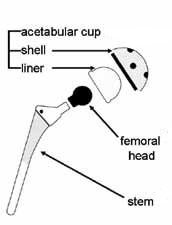
\includegraphics[width=0.5\linewidth]{schematic_scheme_hip_prosthetic.jpg}
\end{figure}
\begin{figure}[ht]
	\centering
	\begin{subfigure}{0.5\linewidth}
		\centering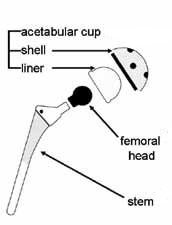
\includegraphics[width=1\linewidth]{schematic_scheme_hip_prosthetic.jpg}
		\caption{\label{fig:fig1}}
	\end{subfigure}%
	\begin{subfigure}{0.5\linewidth}
		\centering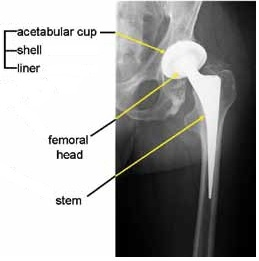
\includegraphics[width=1\linewidth]{Xray_hip_prosthetic.jpg}
		\caption{\label{fig:fig2}}
	\end{subfigure}  
	\caption{\subref{fig:fig1} shows a schematic scheme of the prosthetic and~\subref{fig:fig2} a X-ray image of the prosthesis~\cite{holzwarth2012total}}
\end{figure}
	

{\chapter{Literature review}
An overview of the Total Hip Arthroplasty is given in section 1.1. Section 1.2 informs the reader about the important physiological structures that are important for hip movement. After this, in section 1.3 the indications for THA are listed. Section 1.4 elaborates on preoperative templating and section 1.5 on the most used surgical approaches. Reasons for failure of THA are stated in section 1.6. During the surgery range of motion is measured, section 1.7 explains the importance of this and the limitations and shortfalls of the tools used for this. In section 1.8 the range of motion test during physiotherapy are described. In section 1.9 alignment methods to align the device with the anatomical frame are stated and in section 1.10 the different methods found in literature to fix and IMU on the leg are described. Section 1.11 describes different sterilisation methods for medical devices. With information in section 1.1 to 1.11 a thesis objective and hypothesis is formulated, this can be read in chapter 1.12.

\section{The principle of Total Hip Arthroplasty}
Total Hip Arthroplasty (THA) is a procedure where a defective hip joint with pain symptoms or functional impairment caused by degenerative bone or joint diseases like osteoarthritis is replaced by a hip prosthetic. A modular hip prosthesis design consists of an acetabular cup, femoral head and stem~\cite{holzwarth2012total} as shown in Figure 1.1. Polyethylene is used for the acetabular cup and consists of a shell and liner. The shell is anchored into the pelvis joint and has a liner inserted that functions as a load-bearing layer between the femoral head and the shell. The femoral head is attached to the stem and is inserted in the femur. Fixation of the stem can be done by using acrylic bone cement or by a press fit~\cite{holzwarth2012total}. Cemented stems must be stiff and have a smooth surface to avoid cement fracture. Non-cemented stems have coated surfaces where newly-formed bone tissue can grow. The materials used for the prosthesis must have low friction and withstand wear and oscillating mechanical load. Materials that can be used are stainless steel, cobalt-chromium-molybdenum or titanium-alloys~\cite{holzwarth2012total}. The customizable design allows different materials with different properties.
% \begin{figure}[ht]
%     \centering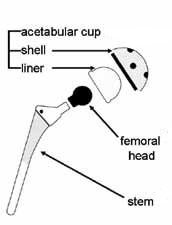
\includegraphics[width=0.5\linewidth]{schematic_scheme_hip_prosthetic.jpg}
% \end{figure}
\begin{figure}[ht]
	\centering
	\begin{subfigure}{0.31\linewidth}
		\centering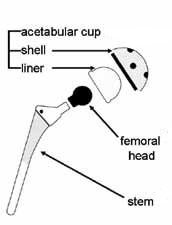
\includegraphics[width=1\linewidth]{schematic_scheme_hip_prosthetic.jpg}
		\caption{\label{fig:fig1}}
	\end{subfigure}%
	\begin{subfigure}{0.31\linewidth}
		\centering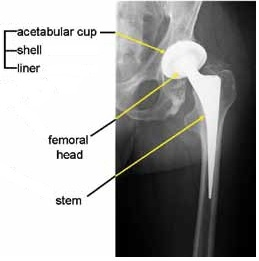
\includegraphics[width=1\linewidth]{Xray_hip_prosthetic.jpg}
		\caption{\label{fig:fig2}}
	\end{subfigure}  
	\caption{\subref{fig:fig1} shows a schematic scheme of the prosthetic and~\subref{fig:fig2} a X-ray image of the prosthesis~\cite{holzwarth2012total}}
\end{figure}

\section{Skeletal frame}
To measure the hip ROM the motion body landmarks need to be identifed. In this chapter the bones of the hip, the muscle that allow movement and ligaments responsible for stability are described. 
\vspace{5mm}
The ROM device is placed before the incision is made in the hip, so the landmarks that need to be estimated need to be accessed from external palpation or visual estimation. The bones of te hip are shown in image 1.2. The ligaments and muscles are shown in image 1.3 and 1.4. The ligaments can be divided in intracapsular and extracapsular ligaments. The intracapsular ligament is the ligament of the head of the femur. The extracapsular ligament is the Iliofemoral ligamengt, the pubefemoral ligament and the Ischiofemoral ligament. 
	
\begin{figure}[!htb]
		\centering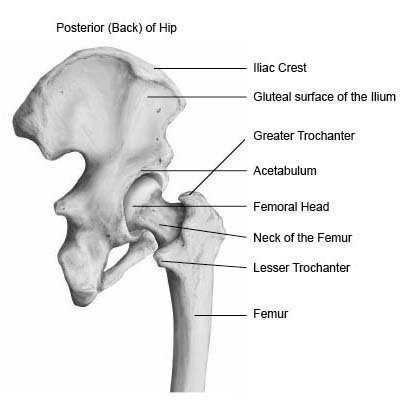
\includegraphics[width=1\linewidth]{hip_bones.jpg}
		\caption{a posterior view of the hip bones~\cite{Hipligaments2018}}
\end{figure}	

\begin{figure}[!htb]
	\centering
	\begin{subfigure}[b]{0.5\linewidth}
	    \centering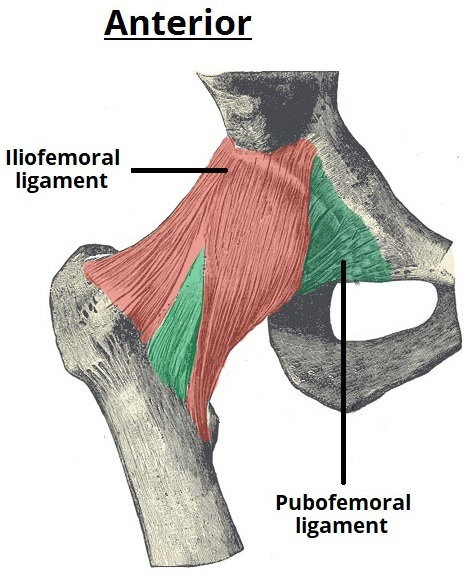
\includegraphics[width=200pt]{hip_ligaments_anterior.jpg}
	    \caption{\label{fig:fig1}}
	\end{subfigure}%
	\begin{subfigure}[b]{0.5\linewidth}
	    \centering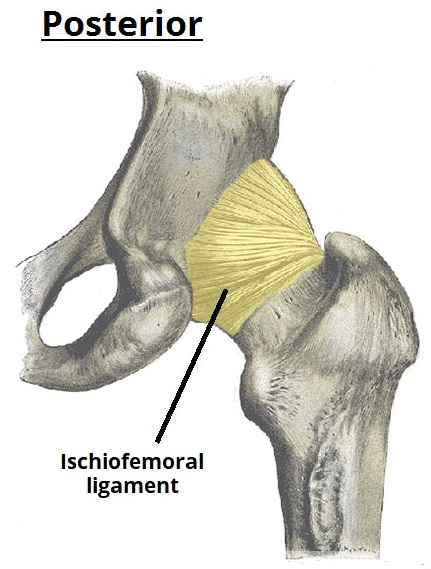
\includegraphics[width=200pt]{hip_ligaments_posterior.jpg}
	    \caption{\label{fig:fig2}}
	\end{subfigure}
	\caption{\subref{fig:fig1} shows the anterior view of the hip ligaments and~\subref{fig:fig2} the posterior view~\cite{Hipligaments2018}}
\end{figure}
\subsection{Motion and muscles}
Listed below are all the possible motions of the hip. Next to them are the principle muscles responsible for these movements:\newline
\textbf{Flexion:}
Iliopsoas, rectus femoris, sartorius \newline
\textbf{Extension}:
Gluteus maximus, semimembranous, semitendinosus and biceps femoris \newline
\textbf{Abduction}:
Gluteus medius, gluteus minimus and the deep gluteals \newline
\textbf{Adduction}:
Adductors longus, brevis and magnus, pectineus and gracillis \newline
\textbf{Lateral rotation}:
Biceps femoris, gluteus maximus, and the deep gluteals \newline
\textbf{Medial rotation}:
Gluteus medius and minimus, semitendinosus and semimembranosus \newline
	
\begin{figure}[!htb]
	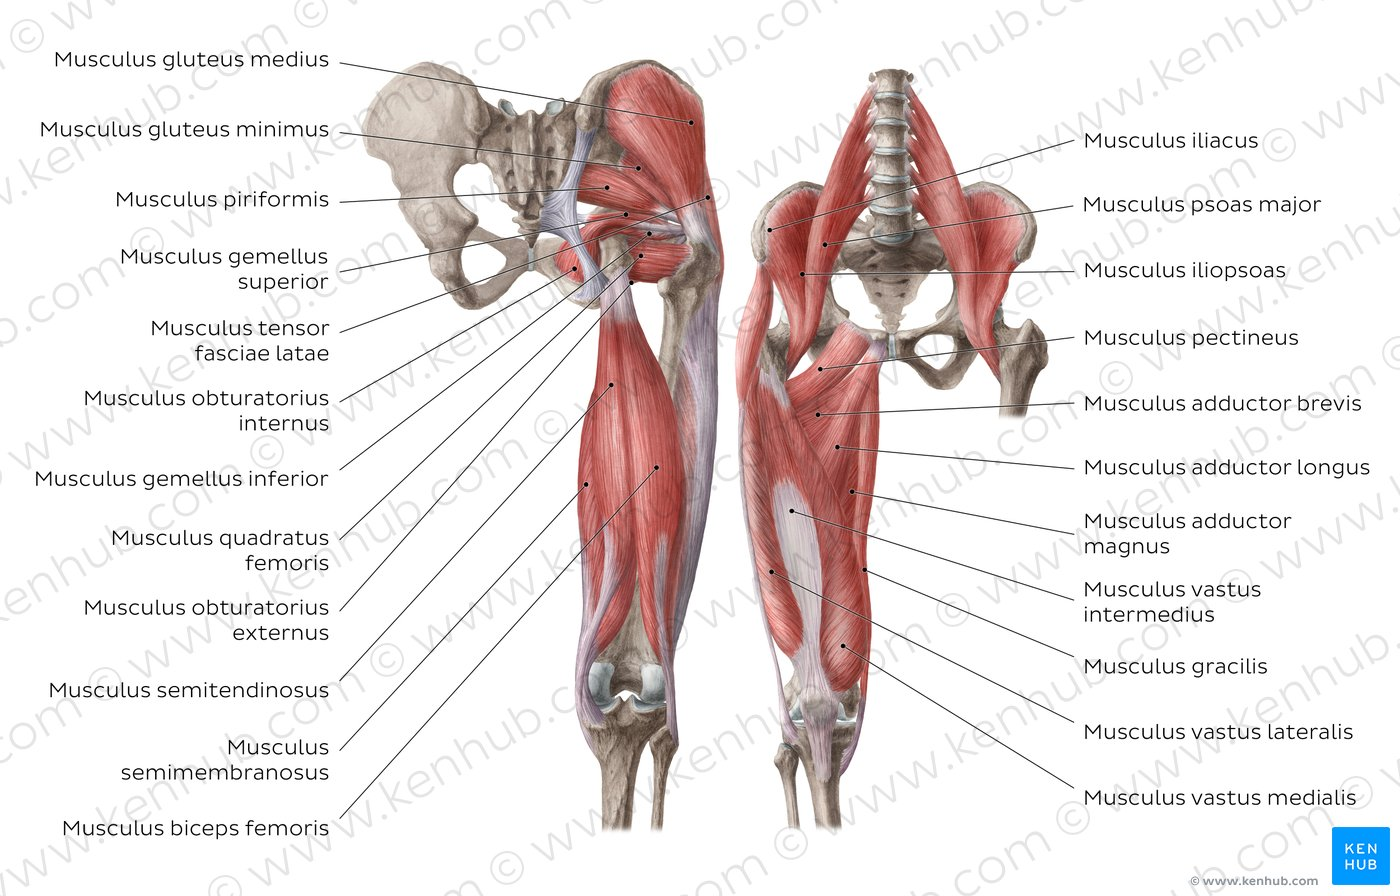
\includegraphics[width=1\linewidth]{hip_muscles.jpg}
	\caption{The muscles involved for movement of the hip~\cite{Hipmuscles2018}}
		\label{fig:my_label}
\end{figure}
%% Use letters for the chapter numbers of the appendices.

\section{Reasons for surgery}
The most common signs for THA surgery are osteoarthritis
(93\%), osteonecrosis (2\%), femoral neck fracture (2\%), developmental dysplasia of the hip (2\%) and inflammatory arthritis (1\%)~\cite{pivec2012hip}. It is a cost-effective treatment in terms of quality of life year gained compared to other common healthcare interventions to regain pain-free mobility in patients with degenerative bone and joint diseases~\cite{holzwarth2012total}~\cite{bozic2004economic}. Osteoarthritis has several causes like femoroacetabular, cam, or pincer-type impingement, especially in young men. The age-standardised (20-89 years) rate of osteoarthritis is 88 per 100000 patients per year ~\cite{oliveria1995incidence}. The diagnosis for performing hip surgery are pain symptoms, functional impairment physical examination and, physical examination of the hip and radiographic findings of the hip joint. There is no general consensus on surgical indications~\cite{pivec2012hip}~\cite{crawford1997total}~\cite{dreinhofer2006indications}. This differs between practitioners, surgeons, and referring doctors, and between countries. THA has a 40\% increased risk of complications for every decade above the age of 65 years~\cite{keener2003twenty}. On the contrary in young people, a group that is more active, the survivorship of the implant is lower because of increased wear and early implant failure~\cite{keener2003twenty}.

\section{Preoperative templating}
Before the surgery, preoperative planning, templating and/or intraoperative navigation takes place. The gold standard for this is an anteroposterior image of the pelvis made with X-ray radiographs~\cite{Pluot2009hip}. Preoperative planning is important because it allows surgeons to determine the prosthesis they should use and the placement location to provide optimal functioning of the joint~\cite{bono2004digital}. An oversized hip joint can result in the fracture of the bone, conversely, an undersized implant can lead to premature loosening of the joint. 
\forceindent The exact amount of limb-length discrepancy can be determined, with the radiographical images of the hipt~\cite{bono2004digital}. The femoral offset of the hip joint can also be measured. The femoral offset is also an important parameter: it determines the moment arm of the abductor's muscles. If the offset is too large the muscles have to generate more force. This can lead to discomfort and earlier fatigue. Over the long term, it can lead to early wear and instability. There is no gold standard for the preoperative templating procedure, however, several studies such as Bono~\cite{ bono2004digital}, Della et al.~\cite{della2005preoperative}, and Scheerlinck \& Thierry~\cite{scheerlinck2010primary} have proposed a systematic preoperative plan that can be used. They vary in the order of steps and anatomical landmarks that are used. The anatomical landmarks are shown in Figure 1.5a. The most important steps are described below:\par

\begin{figure}[!htb]
	\centering
	\begin{subfigure}[b]{0.5\linewidth}
		\centering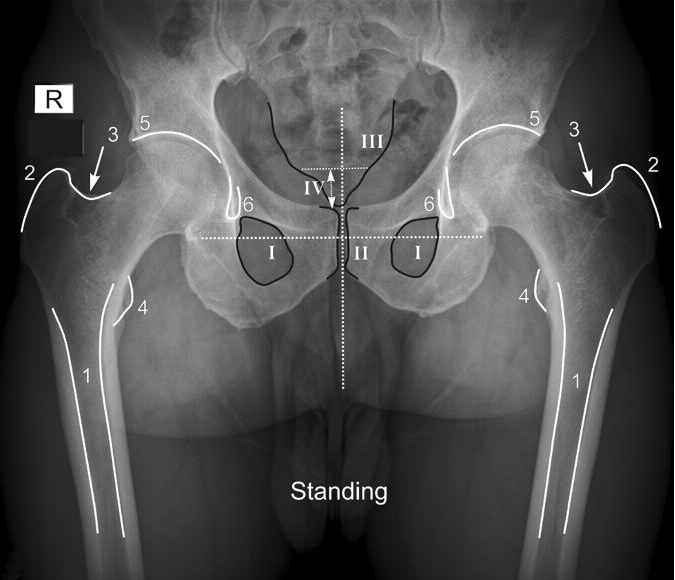
\includegraphics[width=200pt]{preoperativehipscan3.jpg}
		\caption{\label{fig:fig1}}
	\end{subfigure}%
	\begin{subfigure}[b]{0.5\linewidth}
		\centering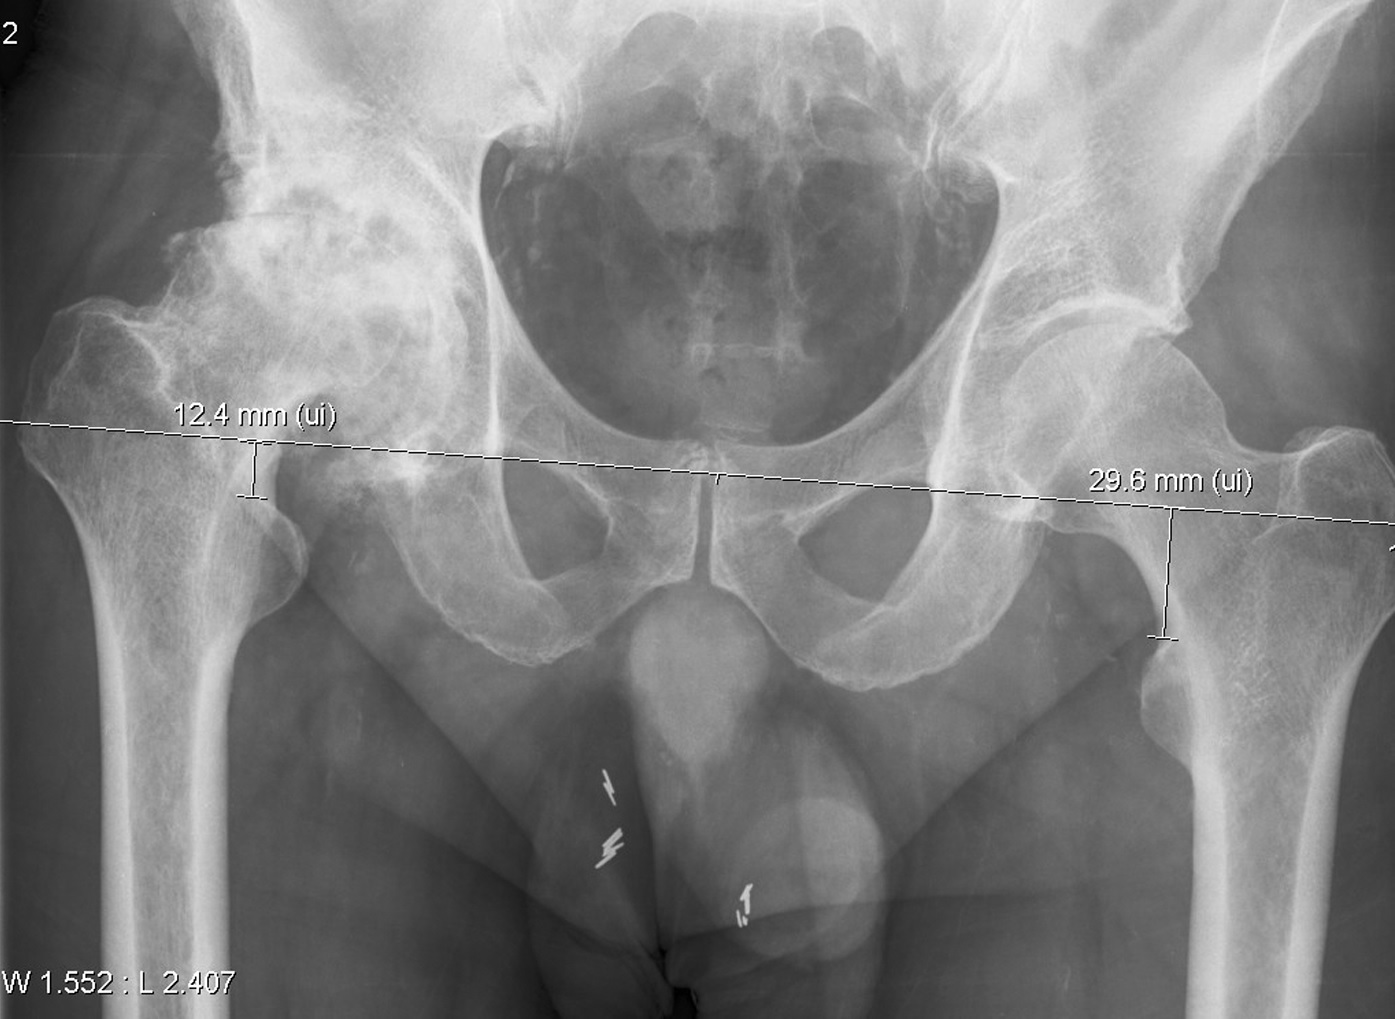
\includegraphics[width=200pt]{preoperativehipscan.jpg}
		\caption{\label{fig:fig2}}
	\end{subfigure}
	\caption{In figure \subref{fig:fig1} all anatomical landmarks are depicted: 1. Femoral shaft; 2. Greater trochanter; 3. “Saddle”; 4. Lesser trochanter; 5. Acetabular roof; 6. Teardrop. Landmarks for radiographic quality assessment : I. Foramen obturatum; II. Symphysis; III. Sacrum; IV. Distance between symphysis and sacro coccygeal joint. In figure \subref{fig:fig2} Limb length is determined by extending a line, perpendicular to the interteardrop axis, to the top of both the lesser trochanter. The difference in measurement equals the limb-length discrepancy~\cite{scheerlinck2010primary} }
	\end{figure}
	\begin{enumerate}
		\item The centre of rotation of the hip joint is determined ~\cite{scheerlinck2010primary}. This done by placing the template with the cup at 40\degree    ~$\pm$ 10\degree~of abduction in the inter-teardrop axis and midway between the inner wall of the pelvis and the subchondral plate of the acetabulum.        
		\item The magnification of the radiograph should be determined by using the measurements of an already existing implant in the body or a radiographic marker with known dimensions ~\cite{ bono2004digital}.   
		\item The orientation of the pelvic axis needs to be determined ~\cite{ bono2004digital}. This is done by drawing a horizontal reference line through the base of both teardrops (figure 1.5b). By knowing this a standard reference can be formed which can be used to compare right and left limbs. 
		\item Leg length discrepancy is determined and if so how large (Figure 1.5b) ~\cite{ bono2004digital}. The top of the lesser trochanter can be used, by measuring the perpendicular distance from the proximal corner to the lesser trochanter fo the reference line.
		\item The size of the femoral component is decided. The appropriate size should fit between the lateral and medial cortex of the proximal femur ~\cite{ bono2004digital}. 
		\item Placement of digital femoral component within the feur that corrects for a discrepancy in leg length and has the right femoral offset ~\cite{ bono2004digital}.
		\item Determinate the leg length of the femoral neck resection needed to place the femoral component in position~\cite{ bono2004digital}.
		\newcounter{enumTemp}
		\setcounter{enumTemp}{\theenumi}
	\end{enumerate}


An alternative for X-ray images is 3D scans made with Computed Tomography (CT). However, it is not used that frequently because it is associated with higher costs and increased radiation exposure~\cite{huppertz2011computed}. The advantage of CT is that no imprecise magnification factors have to be used, as the X-ray beam travels from the object to the film it diverges. To keep the magnification factor consistent, the distance betweenthe hip needs to be positioned at exactly the distance from the source and film for every patient~\cite{scheerlinck2010primary}. However, because patients have different body builds this is hard to control. CT also allows for a depiction of the hip in three planes.  

\section{Surgical approach}
Many surgical approaches are possible for THA. According to Palan et al.~\cite{palan2018surgical}). the most common surgical approach is the posterior approach (62\%), the lateral approach (36\%) and the anterior approach (10\%). Chechik et al.~\cite{chechik2013surgical} conducted a survey on the preferred technique of 292 orthopaedic surgeons in 57 countries and found that the posterior approach (45\%), direct lateral approach (42\%) and anterior approach (10\%) were the most popular ones. The anterior approach has the main benefits that it does not harm the muscle, the patient earlier regains gait and mobility, a lower dislocation rate, clear view of the skeletal landmarks~\cite{palan2018surgical}\cite{petis2015surgical}. The drawbacks are less access to the posterior column compared to the posterior approach, no option to clinically compare leg length intraoperatively, general anesthesia is needed for muscle relaxation and technically demanding~\cite{palan2018surgical}. The internervenous plane, plane where the surgery takes place, lies between the santorius and the tensor fasciae latae. The posterior approach gives a good exposure of the acetabulum and femur. It disadvantage is that is associated with increased dislocation, however recent studies suggest this is not the case. It is also associated with increased risk of sciatic nerve injury~\cite{palan2018surgical}. There is an incidence of 1.3\% when the posterior approach was performed~\cite{petis2015surgical}. The lateral approach has as advantages that it gives a good exposure of the acetabulum and the femur. It also has mimimum risk to damage the sciatic nerve. A big drawback is that that this approach can lead to an injury of the abductor mechanism and can slow rehabilitation~\cite{palan2018surgical}. Sciatic nerve injury is associated with abductor insufficiency, a persistent limp and poorer functional outcome. Damage to the adductor abductor mechanism and limp is a very difficult problem to solve for the surgeon. Around 20\% of the patients experience some abductor insufficiency~\cite{masonis2002surgical}. Because the posterior and the lateral are the most common used approaches these will be eloborated.

\subsection{Posterior approach}	\begin{enumerate}
	\item During the posterior approach the surgeon the patient is laying in the lateral decubitus position. A 5 cm skin incision begins 5 cm distal to the greater trochanter, centred on the femoral diaphysis (Figure 1.6a). It curves 6 cm toward the posterior superior iliac spine for 6 cm. The subcutaneous fat is divided and an incision is made in the fascia lata. After this, the muscles of the gluteus maximus are split~\cite{palan2018surgical}\cite{petis2015surgical}. 
	\item Retractors are placed for a more clear view of the short external rotators. The short external rotators are disconnected as close as possible to its insertion beneath the greater trochanter. To repair them later in the procedure a stay suture is placed in the corner of the excised capsule. Now the femoral head and neck are visible for the surgeont~\cite{palan2018surgical}\cite{petis2015surgical}. 
	\item The surgeon now dislocates the hip out of its joint through gentle flexion, adduction and internal rotation. Neck osteotomy is then performed in the correct orientation according to the preoperative template that was made. Retractors are placed to expose the acetabular. The hip is slightly flexed with the knee in extension, this provides a clear view of the inferior soft tissue to provide a view of the acetabulum, including the transverse acetabular ligament~\cite{palan2018surgical}\cite{petis2015surgical}. 
	\item The femoral head is removed inserting a 'corkscrew' in the femoral head to extract it out of the joint and an orthopaedic spoon in the joint space (Figure 1.6b). The acetabulum is reamed out according to the preoperative plan. If the acetabular preparation is completed the acetabular component can be inserted~\cite{palan2018surgical}\cite{petis2015surgical}. 
	\item After this, the proximal femur is exposed by internally rotating, flexing and slightly adducting the leg. The opening of the proximal femur is done by broaching in the femoral canal to the required size. A trial 'stem' is inserted and the distance from the lesser trochanter to the cone is measured and compared to the preoperative planning. If this is correct the surgeon connects the hip joint to the femur~\cite{palan2018surgical}\cite{petis2015surgical}.
	\item The surgeon can assess the soft tissue tension. If this is not correct he can choose a neck with a higher offset or choose a neck with a smaller neck-shaft angle to lateralise the femur. On average the trial head needs to be switched two times per surgery. The reasons why this may be needed are inaccuracies that can occur when performing osteotomy at the femoral neck, the stem can be placed too deep or to stem lays to superficial~\cite{blaauw_2018}. The hip stability is also assessed by bringing the leg in extension and flexion at varying degrees of rotation~\cite{camenzind2018direct}. 
	\item The definite components are placed. Wound lavage is performed and the surgical layers a closed. 
\end{enumerate}

\begin{figure}[ht]
	\centering
	\begin{subfigure}[b]{0.5\linewidth}
		\centering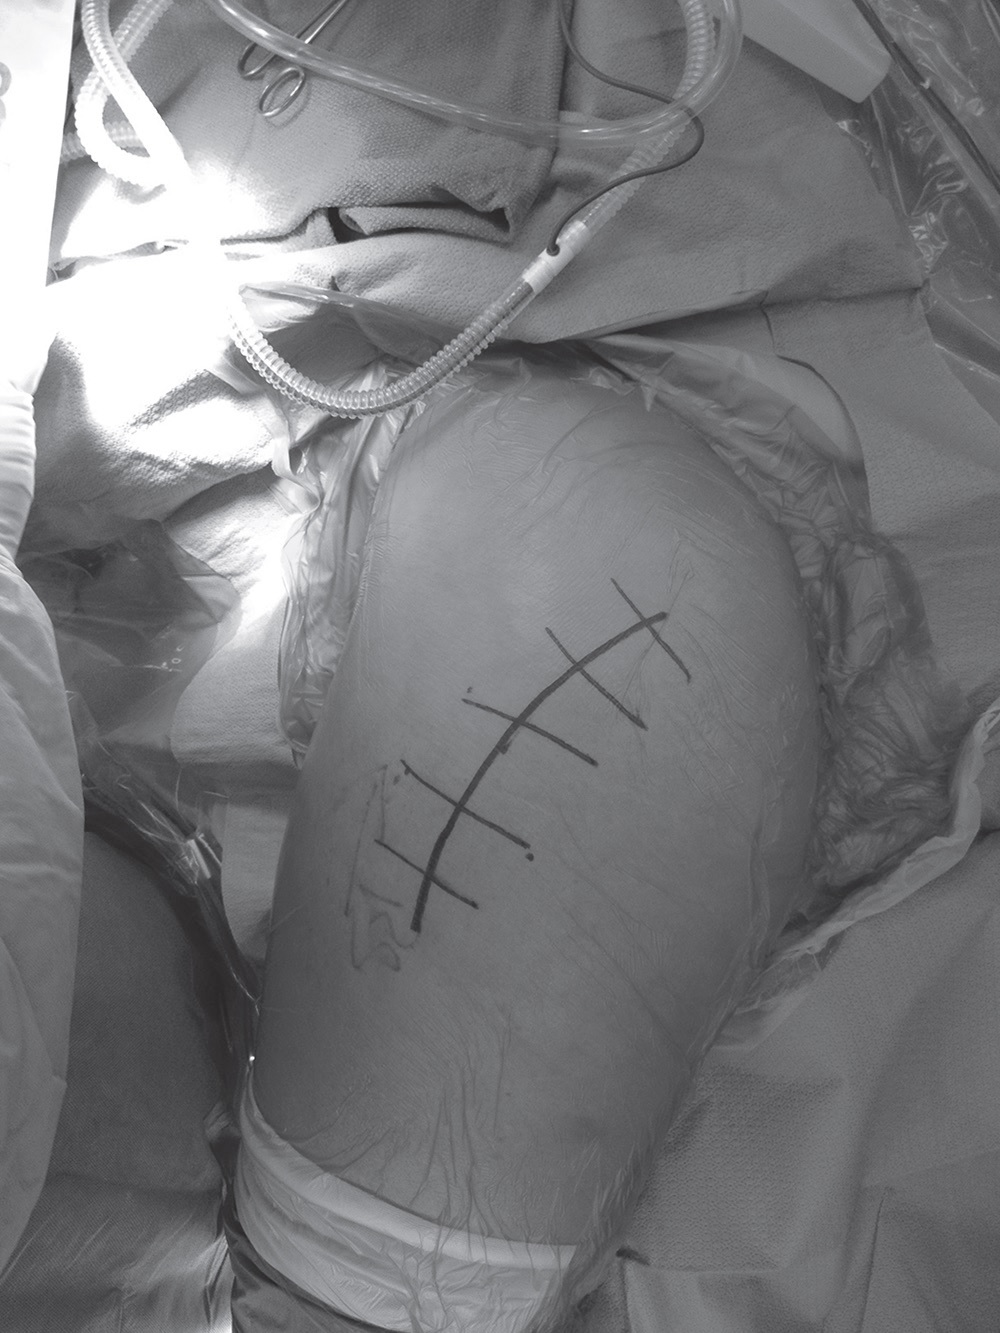
\includegraphics[width=200pt]{skinincision.jpg}
		\caption{\label{fig:fig1}}
	\end{subfigure}%
	\begin{subfigure}[b]{0.5\linewidth}
		\centering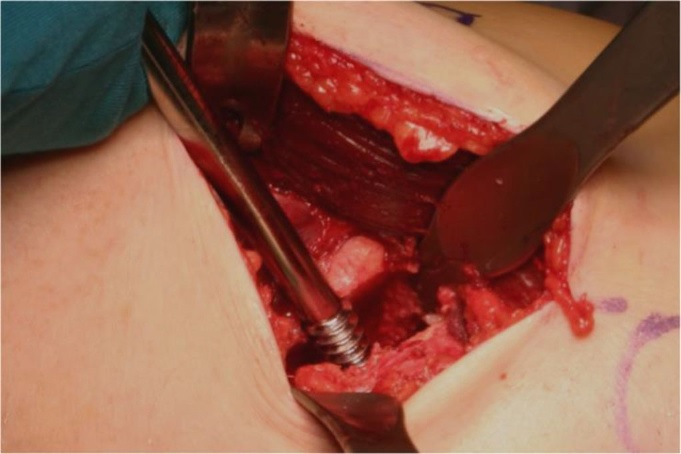
\includegraphics[width=200pt]{removingfemoralhead.jpg}
		\caption{\label{fig:fig2}}
	\end{subfigure}
	\caption{\subref{fig:fig1} shows the skin incision during the posterior appraoch and~\subref{fig:fig2} the corkscrew and orthopedic spoon~\cite{camenzind2018direct}~\cite{petis2015surgical}}
\end{figure}

\subsection{Lateral approach}
\begin{enumerate}
	\item The patient needs to be placed in the lateral decubitus position to place the implant in the right orientation, to correct for leg length discrepancy and cementing (Figure 1.7a). The operative leg is draped and placed into a sterile bag. This allows the surgeon to dislocate the hip and to visualize the femur during preparation without contaminating other areas of the body~\cite{palan2018surgical}. 
	\item An incision is made centred over the greater trochanter that extends distally 5-8~cm in the line of the femur and proximally 3-5 cm straight or with a very slight posterior curve (Figure 1.7b). The fascia is split between the tensor fascia lata and gluteus maximus muscle fibre (Figure 1.7c)~\cite{petis2015surgical}.
	\item The tendon and muscle fibres are split in the centre of the most anterior and posterior extent of the muscle. The gluteus minimus is split in line with the neck of the femur or in the line of the fibres of the gluteus minimus. 
	\item The femoral head is dislocated from the acetabulum by externally rotating and flexing the femur. Hohmann retractors are placed around the femoral neck to provide sufficient visualization. Femoral neck osteotomy with an oscillating saw is performed. After this, the surgeons can reach the acetabulum and proximal femur~\cite{petis2015surgical}~\cite{palan2018surgical}.
	\item The acetabulum is prepared. This is done by externally rotating the leg in extension on the table. The proximal femur is prepared by externally rotating the hip and flexing the hip to near 90\degree. The leg is placed in a sterile anterior 'leg bag'~\cite{palan2018surgical}. 
	\item If the preparation of the procedure is done the femoral head is removed and the prosthetic components are placed in the same manner described in steps 4-7 of the posterior approach~\cite{palan2018surgical}~\cite{petis2015surgical}. 
\end{enumerate}

\begin{figure}[ht]
	\centering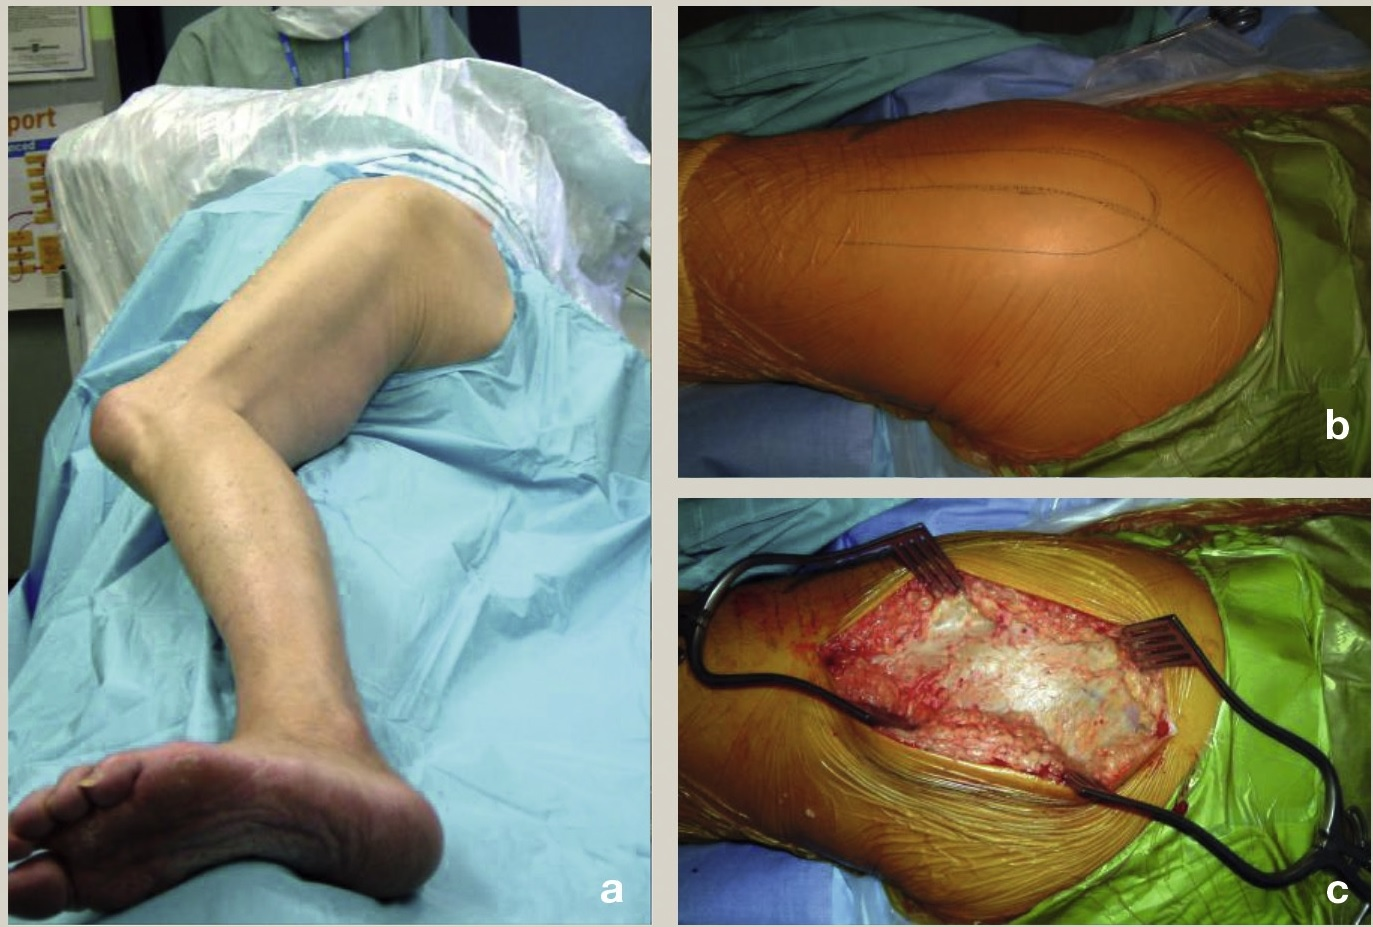
\includegraphics[width=260pt]{lateral_approach_beter.jpg}
	\caption{(a) the setup; (b) the location for the skin incision; (c) the fascia.~\cite{palan2018surgical}}
\end{figure}

\section{Failure in total hip arthroplasty}
The most frequent causes of failure of THA are as follows: aseptic loosening (51.9\%), instability (16.9\%) and infection (5.5\%)~\cite{ulrich2008total}. Most common reasons for revision according to Jafari et al.~\cite{jafari2010revision} were as follows instability (22\%), mechanical loosening (20\%) and infection (15\%). The causes and clinical consequences of aseptic loosening and instability are described below. 
\subsection{Dislocation}
Instability of the hip prosthesis leads to dislocation. Dislocation happens if the head of the prosthesis moves away from the acetabular component. The most common cause of dislocation is impingement by the prosthesis (Figure 1.8a) or bone (Figure 1.8b)~\cite{zahar2013dislocation}).
Polyethylene in the acetabular cup creates a resistive moment to the femoral head which prevents it from dislocation. The contact point of impingement causes an external loading. If the external loading is too high dislocation occurs (Figure 1.8c). %	
Impingement occurs when there is contact between the metal femoral neck and the cup liner or bone-to-bone contacts like the greater trochanter and the pelvis~\cite{malik2007impingement}. Common causes for this are design features like a reduced head-neck ratio and the presence of an extended-rim liner.  
Clinical outcomes of impingement are dislocation, pain, increased wear, loosening of femoral and acetabular components.

	
\begin{figure}[ht]
	\centering
	\begin{subfigure}{0.33\linewidth}
		\centering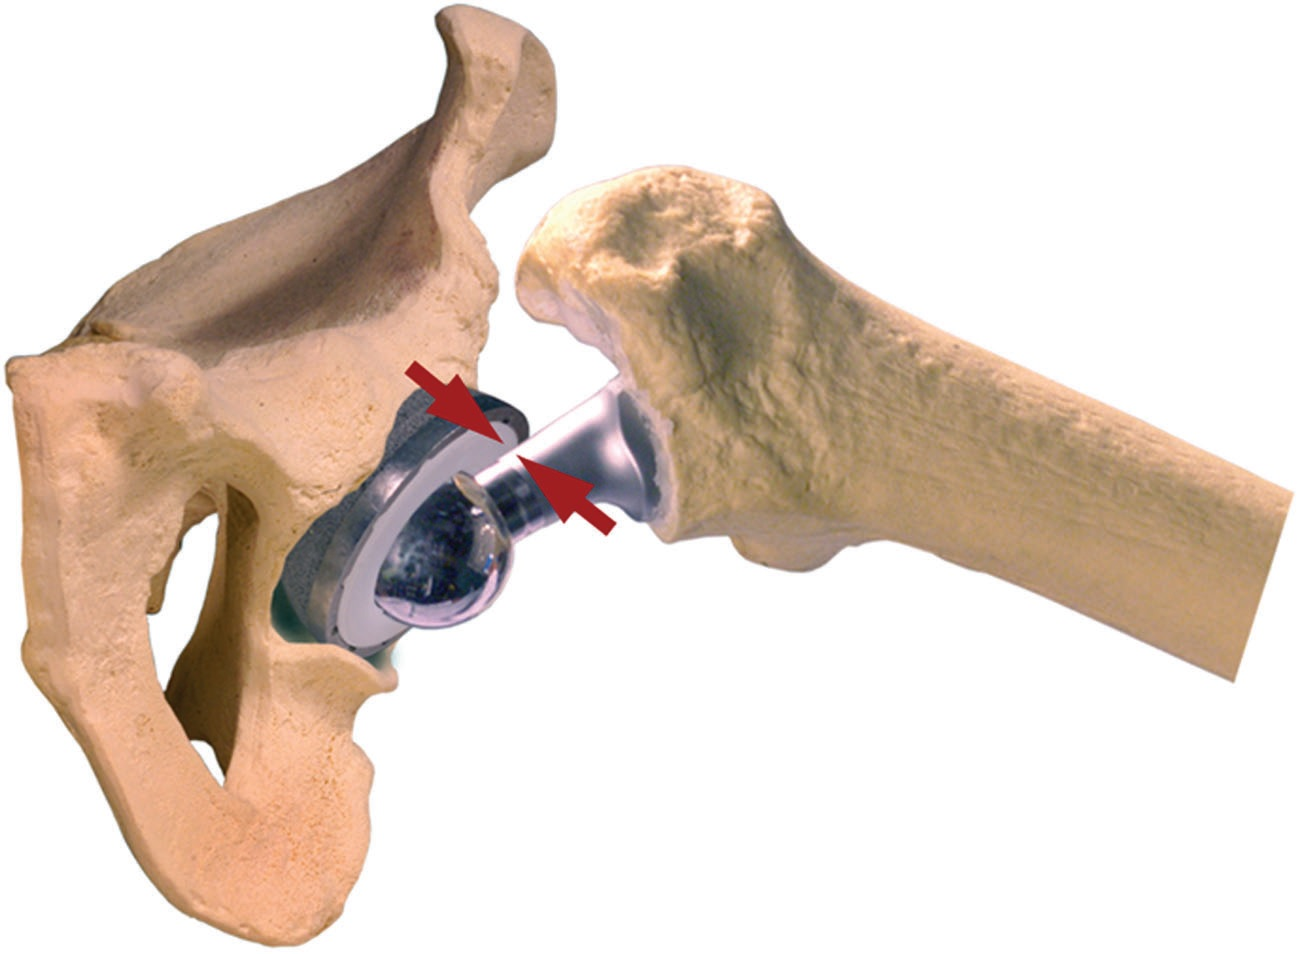
\includegraphics[width=150pt]{hipinpingement1.jpg}
		\caption{\label{fig:fig1}}
		\end{subfigure}%
		\begin{subfigure}{0.33\linewidth}
		\centering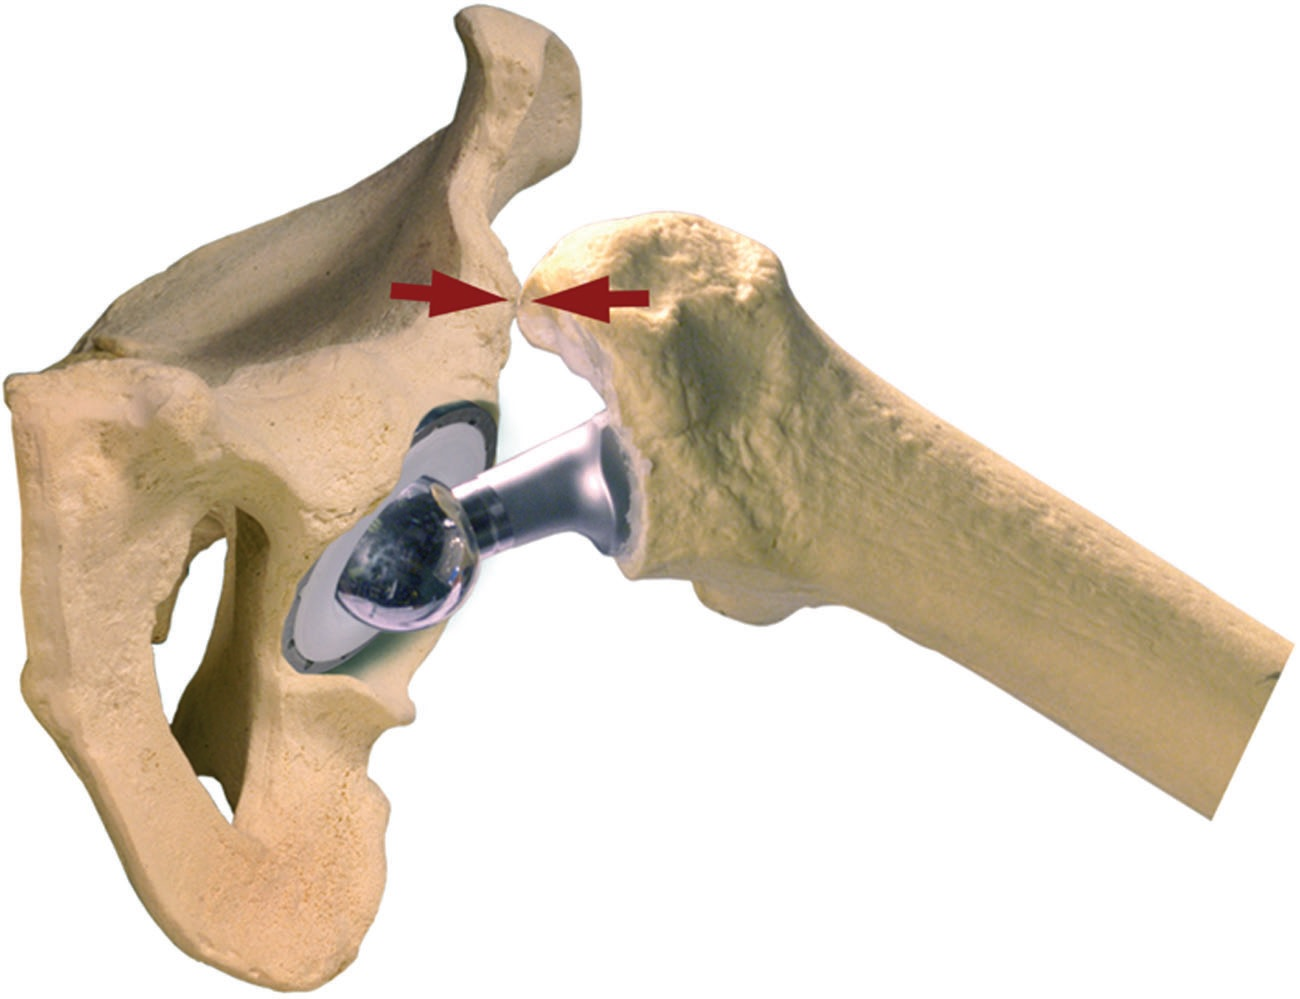
\includegraphics[width=150pt]{hipinpingement2.jpg}
		\caption{\label{fig:fig2}}
	\end{subfigure}
	\begin{subfigure}{0.33\linewidth}
		\centering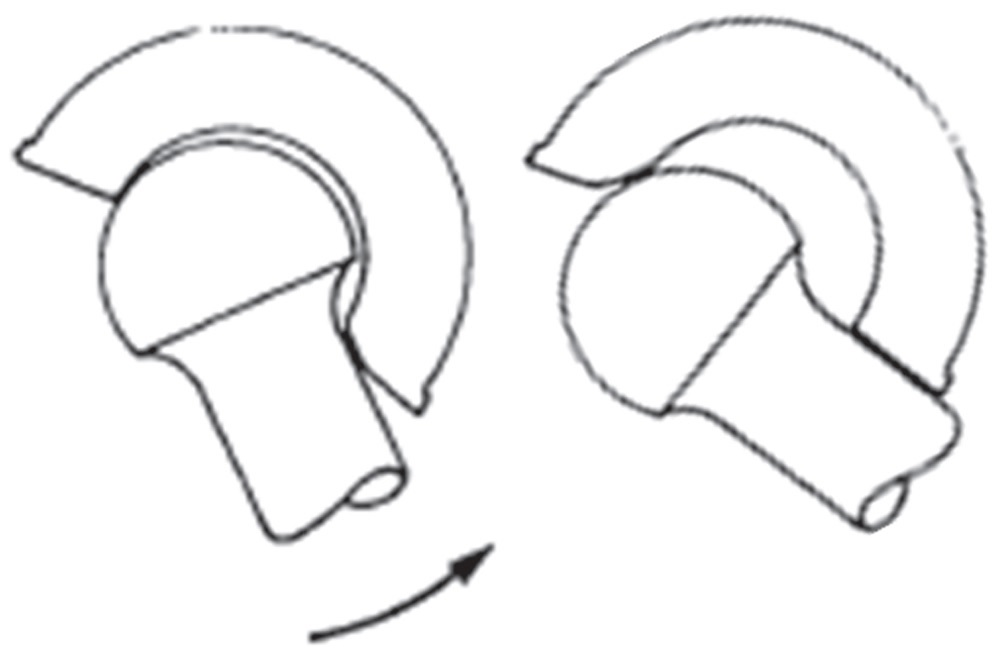
\includegraphics[width=150pt]{Dislocation.jpg}
		\caption{\label{fig:fig3}}
	\end{subfigure}
	\caption{(\subref{fig:fig1}) and(~\subref{fig:fig2}) show how impingment can occur and~(\subref{fig:fig3}) how it can lead to dislocation}
\end{figure}
Surgeons can prevent dislocation by providing an impingement-free range of motion. This can be done by positioning the prosthesis with correct combined acetabular and femoral anteversion and an optimal head-neck ratio~\cite{biedermann2005reducing}. Larger femoral heads are also associated with greater hip ROM and joint stability~\cite{burroughs2005range}~\cite{pivec2012hip}. 

	
\subsection{Aseptic Loosening}
Aseptic loosening is a common cause of failure in THA. Aseptic loosening is a mechanical failure of the prosthesis-host interface~\cite{pivec2012hip}. The pathogenic mechanism is osteoclast-mediated bone resorption at the bone-implant interface, which can lead to loosening, implant migration, implant failure or periprosthetic fracture. Component malpositioning, activity level, material and component design effect on aseptic loosening. 
Risk factors for aseptic loosening can be divided into patient factors, prosthesis factors and surgical factors~\cite{macinnes2012risk}. Patient factors associated with a higher risk are obesity, having an active lifestyle and genetics. The prosthesis risk factors are related to the design, wear rates and the material used for the bearing couple. Surgical risk factors are hospital type and the frequency the surgeon performs THA, the prosthesis alignment, the stability of the prosthesis and the cemented technique used.
	Aseptic loosening can be treated with replacement of components that are detached and correction of any component malalignment~\cite{pivec2012hip}. Replacement of the femoral stem shows favourable results~\cite{khanuja2011cementless}\cite{jones2004modular}. Acetabular revision needs supplementary interventions like the use of jumbo cups, bone grafting, acetabular cages or highly porous metallic augments.
	
\section{Range of motion analysis in total hip arthroplasty}
The range of motion (ROM) assessment is performed during surgery to determine the success of hip surgery~\cite{harris1980advances}. A limited ROM is associated with a greater dislocation risk~\cite{tanino2018hip}. The methods and equipment to assess ROM, the importance, the limitations and alternatives are described below.
	
\subsection{Assessment of hip range of motion}
The range of motion is tested in two patterns: flexion and internal rotation; extension and external rotation. The authors defined the surgery as successful if the leg can move 30\degree~external rotation with full extension, flex to 110\degree~and 20\degree~of internal rotation while the hip is at 90\degree~flexion~\cite{harris1980advances}. If impingement occurs the surgeon has to estimate if it lies in the range of motion for activities of daily living~\cite{woerner2016visual}. If this is the case he has to change the implant orientation, offset increase or remove osteophytes that hinder ROM. Visual estimation is the most used method to evaluate the ROM of the hip after THA~\cite{chevillotte2009variability}, it is a fast method and no equipment is needed. Another common tool to evaluate the RoM of the Hip is a goniometer~\cite{mohsin2015factors}. Different types of goniometers exist like the universal goniometer (Figure 1.9a), an electrical goniometer (Figure 1.9b) and a gravity-dependent goniometer with the universal goniometer being used most often~\cite{roach2013concurrent}. 
	
\begin{figure}[ht]
	\centering
	\begin{subfigure}[b]{0.5\linewidth}
		\centering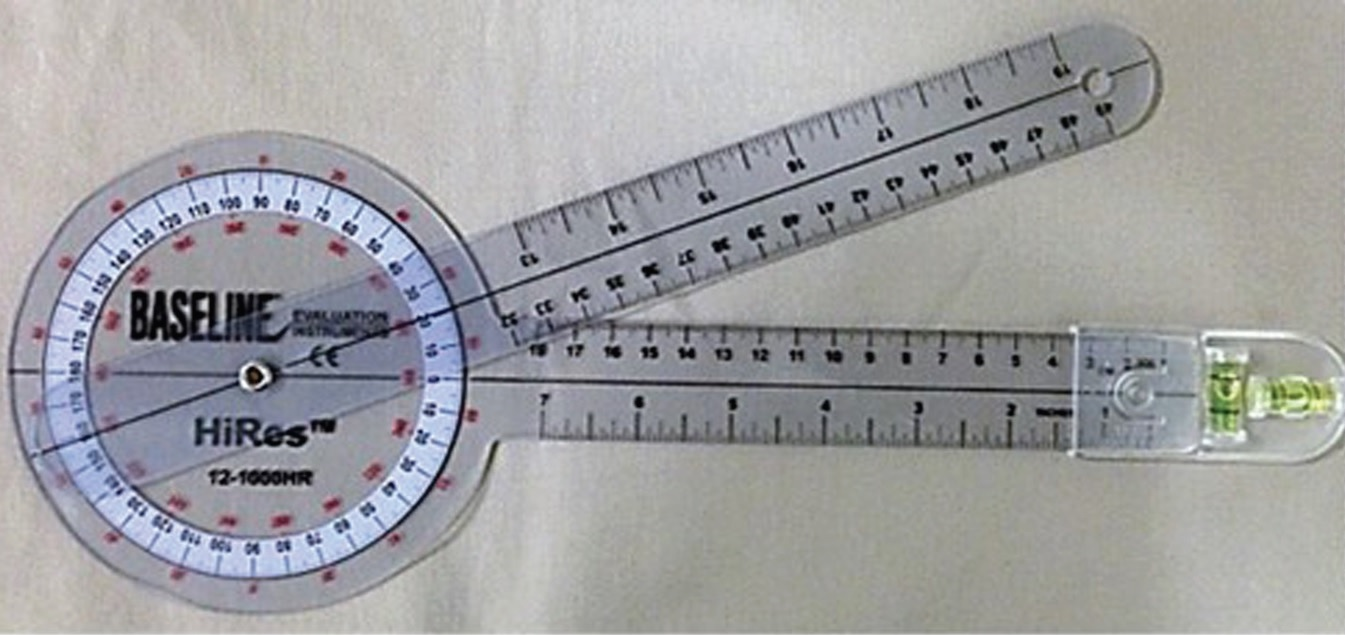
\includegraphics[width=200pt]{goniometerA.jpg}
		\caption{\label{fig:fig1}}
		\end{subfigure}%
		\begin{subfigure}[b]{0.5\linewidth}
		\centering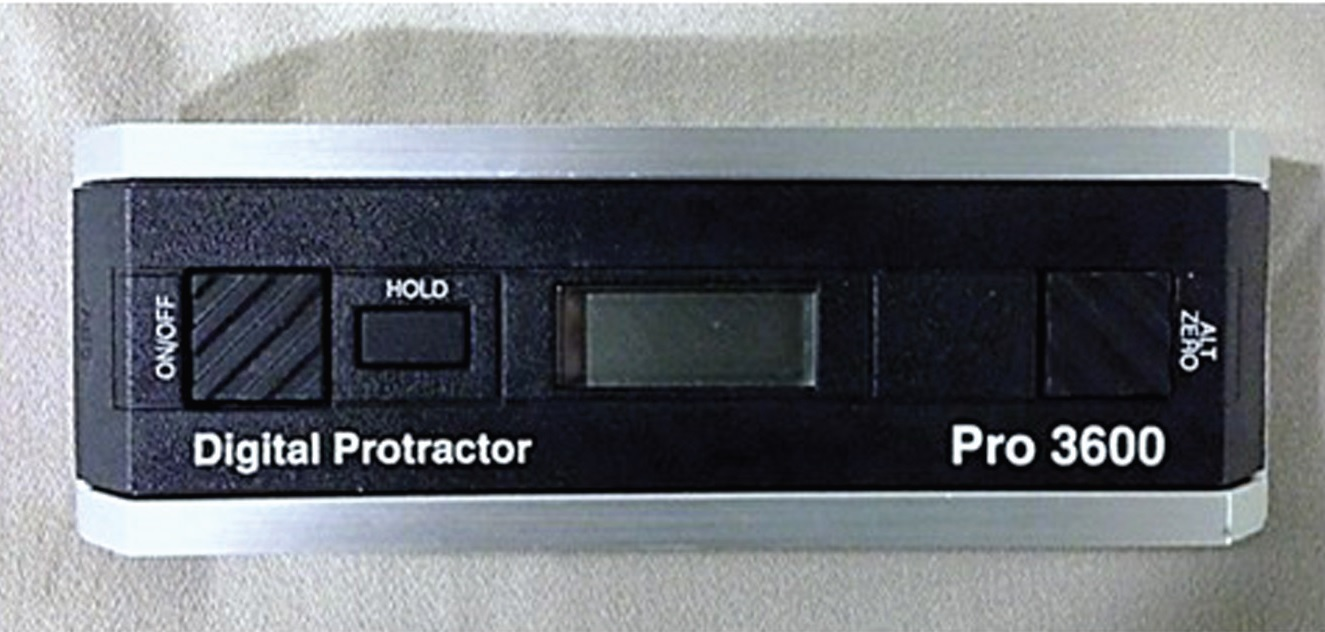
\includegraphics[width=200pt]{goniometerB.jpg}
		\caption{\label{fig:fig2}}
		\end{subfigure}
		\caption{(\subref{fig:fig1}) shows the universal goniometer and~(\subref{fig:fig2}) the electrical goniometer}
\end{figure} 
	
The importance of ROM assessment, however, is still questionable~\cite{davis2007importance}. Widmer\&Zurfluh~\cite{widmer2004compliant} found that a correct combination and orientation of prosthetic components will return a maximized, stable range of motion. Different hip rating methods are available to score hip function after THA like the Harris Hip score~\cite{harris1969traumatic}, the Mayo Hip score~\cite{singh2016validation}, Charnley Hip score~\cite{charnley1972long} and the Merle d'Aubigne Hip score~\cite{d1954functional}. There is low intra-observer reliability between the systems and they vary in the importance given to the range of motion~\cite{callaghan1990assessing}. For example, the Harris hip score includes the range of motion and the Maya Hip score does not~\cite{singh2016validation}. Davis et al.~\cite{davis2007importance} examined the correlation is between the hip range of motion and hip function and how important this is. They defined references for a high, average and low range of motion for flexion/extension, abduction/adduction and internal/external rotation for the hip. They found that hip motion was correlated with hip function. The authors recommended that hip rating systems should give more importance to the range of motion of the hip when determining hip function. No acceptable error was found in literature RoM assessments. A $\pm 5$ $^\circ$ error can be clinically acceptable in some situations, but probably less when definitive clinical decisions are dependent on it~\cite{bruton2000reliability}.
	

\subsection{Limitations of the current method}
Chevillotte et al.~\cite{chevillotte2009variability} examined the reliability of visual estimate and found moderate interobserver and moderate intraobserver reliability when assessing ROM of the hip for flexion, abduction, adduction, internal rotation and external rotation. The authors concluded that visual estimates of hip ROM may lead to substantial errors in the treatment of hip disorders. Woerner et al.~\cite{woerner2016visual} also investigated the reliability of visual estimation of the range of motion by comparing intraoperative assessment by eye with a omputer navigation system (Figure 1.12). The navigation system is further explained in the next paragraph 1.7.3. A mean difference between visual estimation and navigation measurements were for 5.6$^\circ$ for flexion, -0.4$^\circ$ for hip extension, 8.7$^\circ$ for abduction, 5.9$^\circ$ for external rotation and -5.8$^\circ$ for internal rotation. There was a wide range of differences between estimators up to 30$^\circ$. 
\newline
\newline
The universal goniometer also has some drawbacks, it requires the usage of both hands to keep it aligned with the body landmarks while moving the leg and there is low intertester reliability between the identification of the skeletal landmarks and the goniometric alignment~\cite{mohsin2015factors}. The low intertester reliability can be caused by a difference in the force applied by the surgeon for the ROM assessment. Kilgour et al.~\cite{kilgour2003intrarater} investigated the interrater reliability of measurements of lower limb ROM in the sagittal plane in children with spastic diplegia using a goniometer. ROM assessment had lower reliability, the majority of the errors found were most likely related to difficulties in determining the end-range of hip motion. For example, determining the end-range of hip extension before pelvic tilt occurs. However, measurements of the hip joint in a static position correlated with high interrater reliability suggesting proper alignment of the arms of the goniometer with the skeletal landmarks and accurate reading of it. This difference between static and dynamics measurements indicate difficulties keeping the goniometer aligned with skeletal landmarks and correct positioning of the limb when assessing ROM of the hip.Nussbaumer et al.~\cite{nussbaumer2010validity} used the goniometer to asses the reliability of the goniometer. Drawbacks of the goniometer are that the starting position centre of rotation, the longtidunal axis of the limb need to be visually determined. The range of motion of the hip was measured by a goniometer and an electromagnetic tracking system (ETS). The stationary arm of the goniometer was aligned with the horizontal axis of the body and the movable arm with the longitudunal axis of the thigh and the greater trochanter was used as the centre point of the goniometer. The goniometeric measurement were greater when measured with the goniometer compared to ETS. The measurement were most similar for hip abduction and internal rotation, but low for flexion, adduction and external rotation. The difference between the measurement had different causes: pelvic rotation and pelvic tilt that effects the measurement. This causes overestimation of the measurement. Wrong visual estimation and alignment of the true anatomical reference lines which causes an incorrect coupling of the goniometer and the skeletal features. The goniometric measurement also measures two dimensional movement, abduction angle measured in the frontal plane and flexion angle in the sagittal plane may be overestimated by the presence of out-of-plane movements. Mutlu et al.~\cite{mutlu2007reliability} also examined the reliability of goniometric measurements in children with spastic cerebral palsy and concluded that pelvic tilt, alignment of the goniometer with the pivot point, beginning position and velocity of the movement affect the reliability of the measurement. Yazdifar et al.~\cite{yazdifar2013evaluating} compared the goniometer to a motion capture device to measure hip ROM. No significant difference was found, the reason for this is not stated in the article. The optical markers for the camera placed on the body and aligned with the skeletal landmarkers probably made it easier for the user to align the goniometer with the skeletal landmarks.     
\newline
\newline
The inter-observer reliability between different devices is low. There is a discrepancy between visual and goniometric ROM assessment~\cite{holm2000reliability}. Roach et al.~\cite{roach2013concurrent} investigated if there is a difference between measurements of the range of motion on the same patient done with an inclinometer and universal goniometer and found significant differences between measurements.  

\subsection{Alternatives}
An alternative for determining the ROM is an inertial measurement unit consisting of an accelerometer and gyroscope. An inertial measurement unit (IMU) is a micro-electromechanical system consisting of a gyroscope and an accelerometer that allows measurement of the motion of an object attached to it~\cite{bloomfield2018proposal}. A motion of an object can be described by six independent variables~\cite{zeng2011sensing}, linear motion along three different axes and rotational movements around these axes. Most IMUs have tri-axial components allowing measurements in three dimensions. The gyroscope measures the angular velocity and the accelerometer's linear acceleration. Magnetic angular rate and gyroscope are IMU combined with a magnetometer. The magnetometer can measure the direction of earth's magnetic field to help orient the sensor. A more accurate orientation can be achieved, however, estimates can be influenced by external magnetic interference~\cite{lin2012human}. An IMU produces drift over extended use if they do not return to rest. This will result in an error in the reading of the gravity vector~\cite{bloomfield2018proposal}. Measurement sensors can be divided in solid-state and non solid-state motion sensor. Current measurement technologies use solid state motion sensors.
\newline \cite{bloomfield2018proposal}\cite{charlton2015reliability}\cite{renkawitz2012development}

\textbf{Solid state accelerometers}\newline
This type of accelerometers has the structure of a mass-spring-damper system, where the mass is connected to a cantilever to the supporting frame (Figure 1.10). If the system has an external acceleration, an inertial force generates a relative movement between the mass and the supporting frame. This induces a mechanical stress. The movement and the mechanical stress can be used to determine the external acceleration. Many mechanisms use this cantilever system, through capacitive, piezoresistive, piezoelectric or tunnelling current measuring. The three most common accelerometers are the piezoelectric, piezoresistive and capacitive types~\cite{wong2007clinical}. 

\begin{figure}[!ht]
	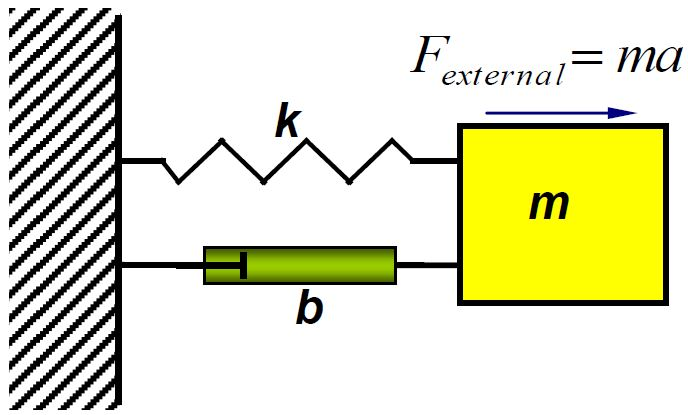
\includegraphics[width=.5\linewidth]{accelerometer.JPG}
	\caption{A second-order mass-spring-damper system representing a cantilever based accelerometer~\cite{zeng2011sensing}.}
	\label{fig:my_label}
\end{figure}

	
Wong et al. \cite{wong2007clinical} recommended piezoresistive and capacative accelerometers for measuring human movement as they can provide dual acceleration components. The capacitive accelerometers have higher stability, sensitivity and resolution than piezoresistive ones~\cite{Gardner1994Microsensors}. During static acceleration, accelerometers can be used to determine the orientation of the device with respect to the earth surfaces~\cite{wong2007clinical}. 
\newline
	
	
\textbf{Gyroscope}\newline
A gyroscope measures the rotary rate of an object by measuring the Coriolis effect~\cite{zeng2011sensing}. This is an imaginary force perpendicular to a subject within a rotating coordinate system. The Coriolis acceleration, proportional to the angular velocity, is an apparent acceleration perpendicular to the movement of a subject in a rotating coordinate system (Figure 1.11a). If a subject is located on the z-axis in a rotating frame with angular rate, \( \Omega\)
the subject will see the movement of the particle along the z-axis with Coriolis acceleration 2*\( \nu\)*\( \Omega\). 
The gyroscope consists of two mass-spring-damper sets perpendicular to each other (figure 1.11b). One set is in drive mode and the other in sense mode. If the y-axis is the drive axis and the z-axis the sense, the displacement along the z-axis is excited by the Coriolis force Fz. The displacement along the z-axis is proportional to the angular velocity. %Ω = xi
\begin{figure}[!htb]
	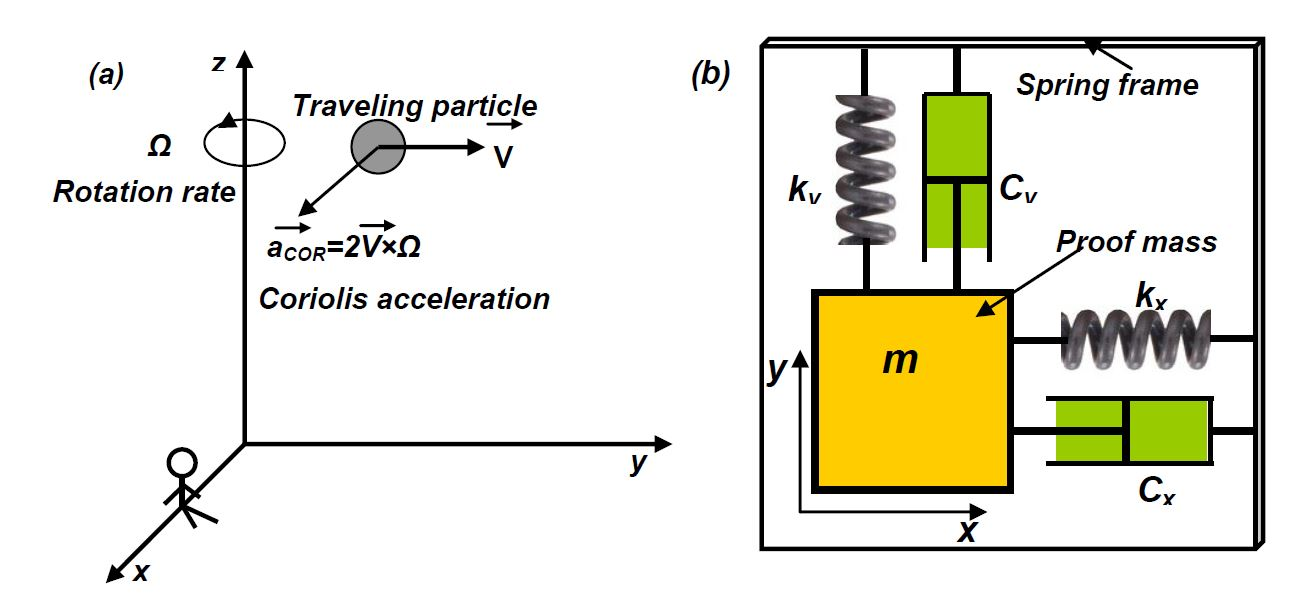
\includegraphics[width=1\linewidth]{gyroscope.JPG}
	\caption{(a) illustration of Coriolis effect;
			(b) the mass-spring-dasher system of a vibratory gyroscope~\cite{zeng2011sensing}.}
	\label{fig:my_label}
\end{figure}

Charlton et al.~\cite{charlton2015reliability} used an IMU of a smartphone to asses the ROM of the hip. The reliability was found to be comparable to a bubble inclinometer. The smartphone in this study was assessed on healthy individuals, and is questionable  whether it can be used during THA. Renkawitz et al.~\cite{renkawitz2012development} developed a computer-assisted impingement detection technique using a navigation system for THA. This is a form of stereotactic surgery that can be used to optimize prosthetic positioning~\cite{kelley2009role}~\cite{renkawitz2009computer}. In this technique, trackers are attached to multiple skeletal landmarks relevant during THA and the computer navigation system detects the spatial relationship of these markers in real time. In the study by Renkawitz et al. fiducial landmarks were placed on the iliac crest, pubic tubercles, greater trochanters, femoral diaphysis and into the femoral condyles ~\cite{renkawitz2012development}. THA was performed and after positioning of the prosthesis, the final position was measured by the navigation system. The navigation system made a 3d image of the implant and bone and calculated the ROM. The system was compared with calculations of ROM by using three-dimensional CT-based models based on the fiducial landmarks made during the surgery. Impingement could be detected with a mean error lower than 5$^\circ$. A drawback of this navigation system could be the cost and that it is too complicated to be used without sufficient training.
	
\begin{figure}[ht]
	\centering
	\begin{subfigure}[b]{0.5\linewidth}
	    \centering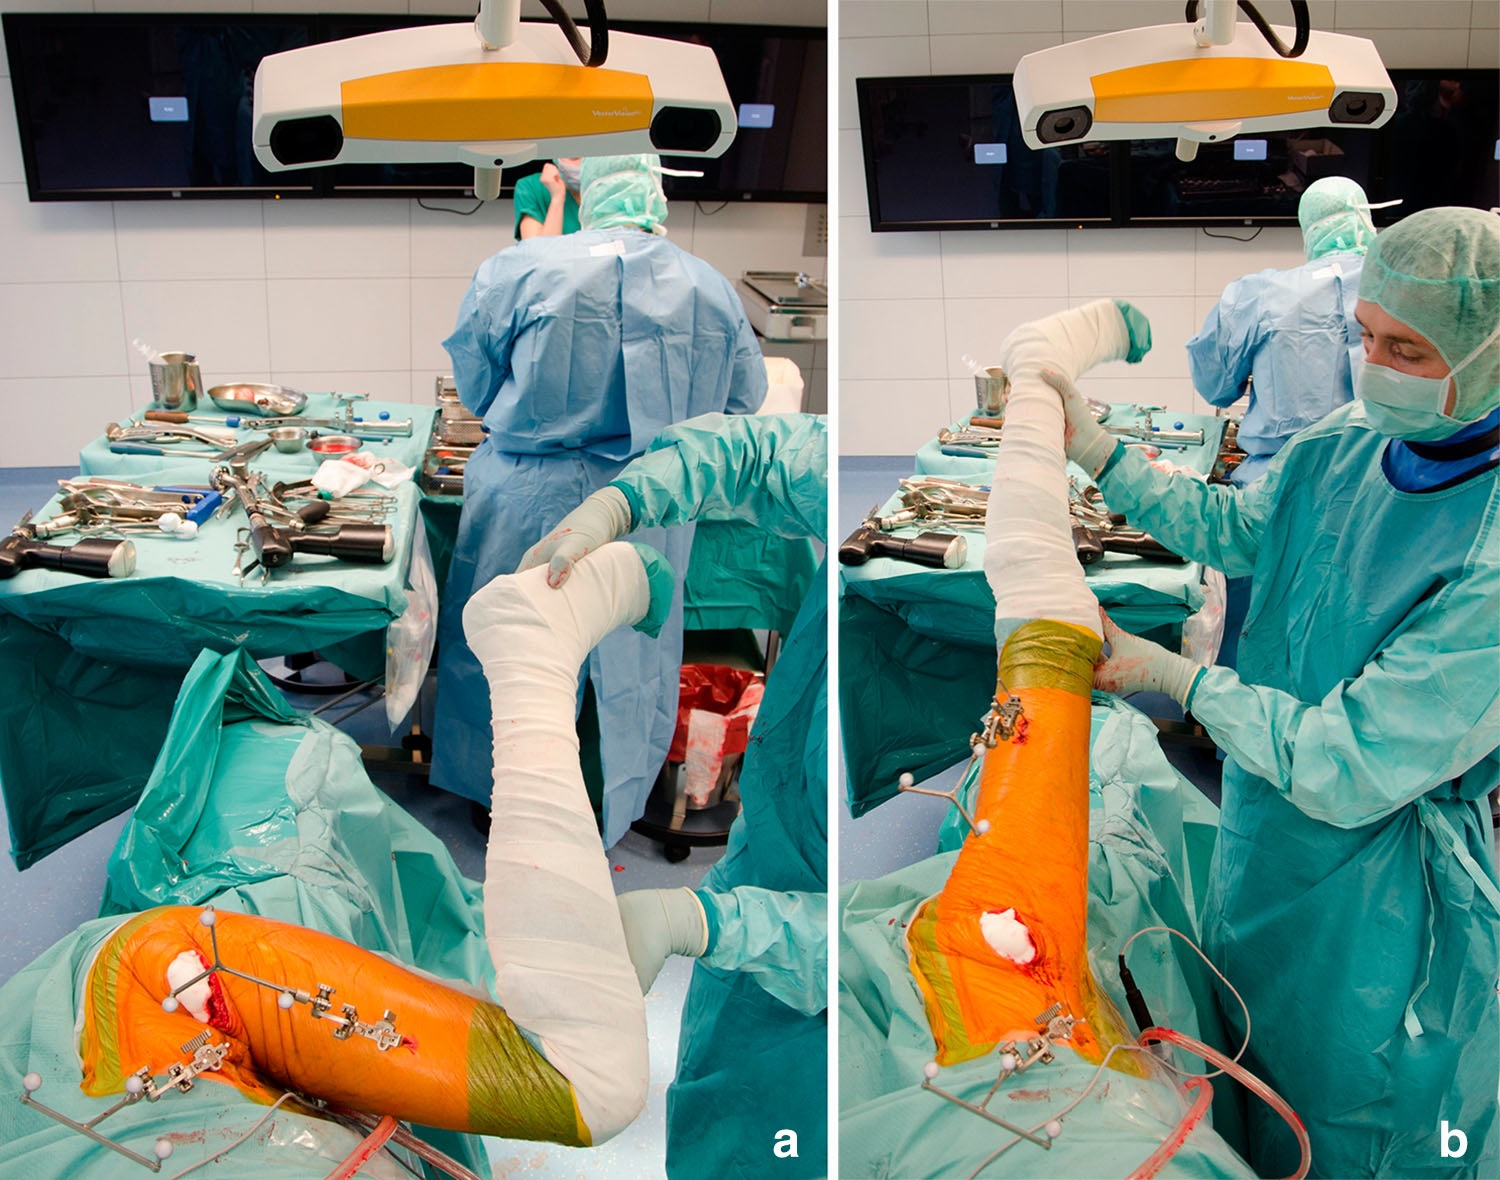
\includegraphics[width=200pt]{rangeofmotionmeasurementusingnavigationsystem.jpg}
	    \caption{\label{fig:fig1}}
	\end{subfigure}%
	\begin{subfigure}[b]{0.5\linewidth}
		\centering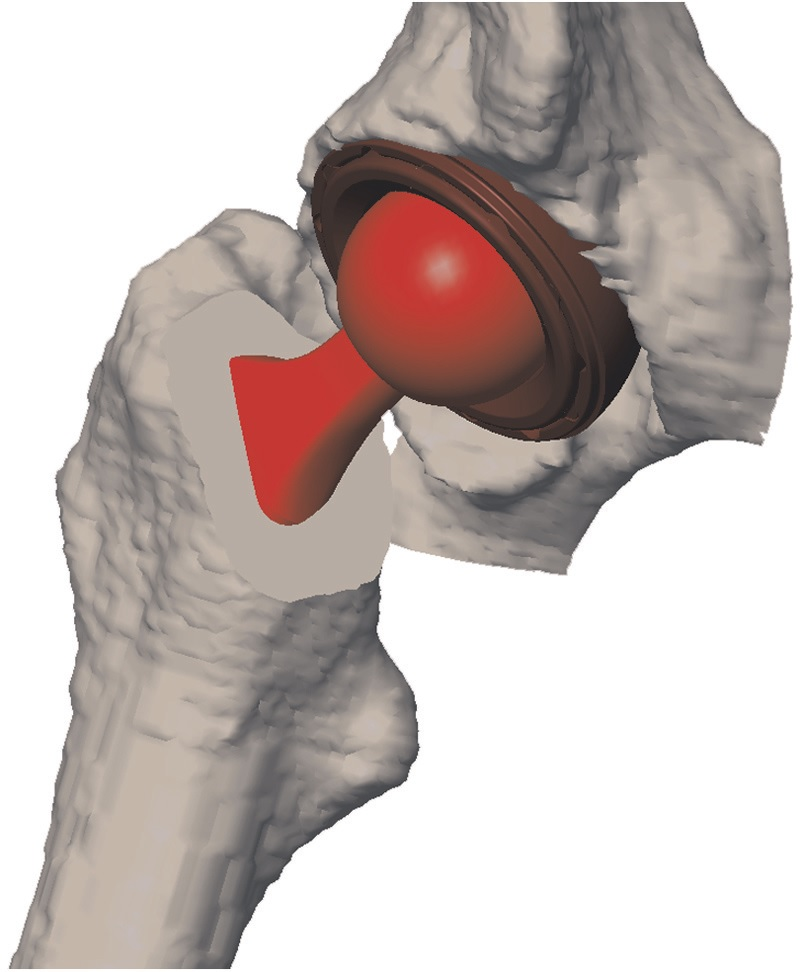
\includegraphics[width=200pt]{computer_navigation_system2.jpg}
		\caption{\label{fig:fig2}}
	\end{subfigure}
	\caption{(\subref{fig:fig1}) shows the assessment of the range of motion of the hip done with the navigation system~\cite{woerner2016visual} and~(\subref{fig:fig2}) the constructed 3D model~\cite{renkawitz2012development}}
\end{figure}

	
\section{Range of motion test during phyiotherapy}
Hip function can be evaluated by different methods. Goniometric measurements are also used during physical therapy to measure ROM of the joints~\cite{gajdosik1987clinical}. The range of motion can be measured by different tools. The most used method during physical therapy is a goniometricmeasurment~\cite{gajdosik1987clinical}.  Ekstrand et al.~\cite{ekstrand1982lower} compared investigated the intrarater variability of hip ROM with a goniometer by comparing it with a more accurate measurement method. This accurate measurement method consisted of covering the examing table with a wood board, standardizing the height of the table, marking skeletal landmarks. They found that the intrater reliability was lower when the goniometer was used. Other factors that make it more difficult when measuring the ROM of motion of the limbs are stretching of soft tissue, the force applied to move the limb~\cite{amis1982elbow} and the type of patient problem. The modified thomas test can be used to assess hip flexibility~\cite{clapis2008reliability}. During the thomas test the patients lies on the table and one leg is lifted till the knee touches the chest. When the leg is lifted 90 \degree the leg is supported externally allowing the patient to relax and standardize the pelvic tilt and lumbar lordotic curve of the spine. During the lift of the leg the right hip can extend freely to allow full extension of the leg. Wakefield et al. \cite{wakefield2015reliability} compared intrarater and interrated reliability for goniometric and trigonometric techniques using the modified thomas test. For the goniometric measurement the proximal arm was aligned with the lateral midline of the pelvis, the distal arm was aligned with lateral midline of the femur and the fulcrum of the goniometer was placed over the lateral aspect of the greater trochanter. For the trigonometric measurement the length was measured between the greater trochanter and the most posterior aspect of the lateral epicondyle of the femur with a standard anthrometric tape. The height of these landmarks was measured from the ground using a stadiometer. The joint angle was calculated using the equation $\theta=\taninv\frac{O}{H}$. The trigonometric method had a higher intra- and interrater reliability.
	
\section{Alignment method}
There are different methods to align the axis of the device with the anatomical frame. It is important that the right anatomical frame is used. Depending on whether the study uses landmarks that are inside or on the body. The reason behind this is that some landmarks are not easy to access from external palpation or visual estimation. This results in different reference systems. Wu. G et al.~\cite{wu2002isb} defined the anatomical landmarks that can be used as the anterior superior ilac spine, the posterior superior ilac spine and the femoral epicondyle. The coordinate system can be defined with the pelvic coordinate system and femoral coordinate system. The centre of rotation can be defined with the hip centre of rotation, this is the origin of the pelvic coordinate system and femoral coordinate system (see figure 13). The z-axis of the pelvic coordinate system is the line connecting the left and right anterior superior ilac spine. The x-axis is a line lying in the plane define by the two ASISs and the midpoint of the two PSISs, orthogonal to the z-axis, and pointing anteriorly (figure 1.13). The Y-axis is the line perpendicular to the X an Z axis. The y-axis of the femoral coordinate system is defined by the midpoint between the medial and the lateral FEs and the origin (figure 1.13). The Z-axis is perpendicular to the y-axis, lying the plane defined by the femoral epicondyle. The x-axis is perpendicular to both y- and the z-axis.
\begin{figure}[!htb]
	\centering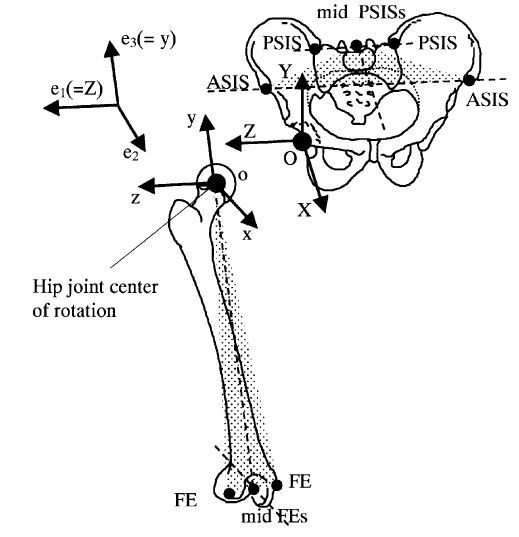
\includegraphics[width=0.5\linewidth]{coordinate_system_hip.JPG}
	\caption{\label{fig:fig1}The pevlic and femoral coordinate system~\cite{wu2002isb}}
\end{figure}%

Vargas-Valencia et al.~\cite{vargas2016imu} proposed an alignment method of the sensor by letting the patient stand stationairy and connecting the device to the pelvis. If this alignment is correct one of the main axis should be aligned with the gravity. This was evaluated by checking the orientation data over a 5 second interval. Each IMU was placed in a box, the orientation of the IMU and the box can have an misalignment of \textless3\degree. Misalingment can affect the results of the measurement. This can be caused by mislocation of the anatomical landmarks which causes an offset of the segment axial rotation. Salehi et al.~\cite{salehi2015body} placed one inertial measurement unit on the upper leg and the other one on the lower leg. With the translation acceleration, angular velocity and angular acceleration the position of the IMUs can be estimated with respect to the knee joint. This results in a optimization problem where a weighted least squares method is used to solve it. Bakhshi S. et al ~\cite{bakhshi2011development} placed two IMUs on the upper and lower leg. The IMUs were calibrated on a flat surface parallel to the ground. In this way the sensors have the same reference coordinator. Bluetooth was used to transfer the data to the pc. The difference in orientation was used to determine the knee angle. 


\section{Fixation method} 
IMUs can be fixed in multiple ways on the leg. Zugner et al.~\cite{zugner2019validation} used elastric straps to connect IMU sensors on the lateral part of the thighs an aligned them with the pelvis. The IMU measured sagittal plane and frontal plane motions. The measured data of the IMU did not fully correspond with the pelvic motion. Main reasons for this are the soft tissue motion around te pelvis, wrong definition of skeletal landmarks on the skin or change in this position when the hip moves in different directions and pelvic tilt. Bergmann et al.~\cite{bergmann2009portable} also used elastic straps and double sided adhesive tape to fix the IMUs on the tensor fascia latae. To align the device with the skeletal frame the x-axis was initially aligned with the sagital plane during stance. The z-axis was aligned with the gravity vector. Bakhshi et al.s~\cite{bakhshi2011development} used a strap to connect an IMU to the leg on the anterior side of the upper and the lower leg to determine lower limb kinematics. Vargas-Valencia et al.~\cite{vargas2016imu} used IMU's that were positioned on the lower limb. The IMU's on the thigh were fixed with either double-sided tape or with elastic cuffs wrapped around the legs. Nussbaumer et al.~\cite{nussbaumer2010validity} positioned the electromagnetic tracking sensors on the thigh and fixed them with velcro straps to minimize the movement between underlying skind and the skeletal features. 


\section{Sterilisation}
Sterilisation is needed to prevent the risk of infection~\cite{tessarolo2008sterilization}. Contamination of medical devices can lead to complications after the intervention. Sterilisation is, therefore, a mandatory process. The World Health Organisation defines sterilisation as any chemical or physical process that implies the destruction of all living forms, including bacteria, fungi, virus, and spores. Different sterilisation procedures exist for every type of instrument. The sterility assurance level is defined by finding living micro-organisms in the sterilisation load after treatment, this should be lower than 10-6. By reviewing the different existing methods the most suitable design can be chosen that allows sterilisation for multiple methods. Different techniques are the use of saturated steam, dry heat sterilisation ethylene oxide, ionising radiation and low-temperature plasma in vapour or gas phase. 

\begin{enumerate}
	\item \textbf{Saturated steam} Steam sterilisation is a process where heat is transferred by condensing steam under pressure. The humid
	heat causes proteins and DNA of micro-organisms to denature. The device should be placed in a packaging material that protects the content, allows for removal of air and penetration of steam. For this purpose sterilisation paper is used. After sterilisation the steam autoclave is brought to vacuum to dry the device and the packaging~\cite{bouwman2015practical}. Saturated steam happens at a temperature between (121-134 \degree C) and (1.1-2.1 bar). It is the most commonly used technique in the hospital. This technique has been used for different biomedical polymers~\cite{tessarolo2008sterilization}. An autoclave is used for the sterilisation. First air is removed by repeated pre-vacuum, then the area is heated and pressure is build through steam insufflation. This will continue to sterilised the device, after this the steam is removed and the device is dried by post cycle vacuum.  
	\item \textbf{Dry heat sterilisation} Dry heat sterilisation is a process where microorganism are destroyed through oxidation, volatilisation of light components and deep dehydration of microorganisms. This happens at a temperature ranging between (150-170 \degree C) for a prolonged time (60–150 minutes)~\cite{tessarolo2008sterilization}. Dry heat is used to sterilise materials that are heat-resistant or cannot come in contact with water or steam. The air is heated by the use of
	electrical heating elements. The disadvantage of dry heat sterilisation is that is less efficient than saturated steam, the sterilisation temperature is higher and the time is longer~\cite{bouwman2015practical}. 
	\item \textbf{Ethylene oxide sterilisation} Ethylene oxide sterilisation is used for thermosensitive products. The procedure includes a vacuum phase in the autoclave and injection of Ethylene oxide gas. An advantage is that no high temperatures are needed, a downside is that post aeration is needed for detoxification of gas residual is needed that can last from 12 hours in forced systems to 14 days when happened spontaniously. ETO sterilisation is suitable for medical devices due it's low temperature~\cite{tessarolo2008sterilization}.  %How can the device stay aligned with those bony landmarks? 
	\item \textbf{Ionising radiations} Sterilisation can also happen with ionising gamma radiation. Ionising radiation consist of lots of energy and can therefore inactivate micro-organisms. This can be performed at room temperature and is time-effective. Around 40\% of the medical devices are sterilised by ionising radiation~\cite{bouwman2015practical}. A drawback of this technique is that it is limited by the investment that is needed to realise the treatment and the management of radiation hazards~\cite{tessarolo2008sterilization}.
	\item \textbf{Steam formaldehyde} Blowing of steam formaldehyde can also be done to sterilised instruments. It is performed at 0.1 bar with injections of saturated steam and vaporised formalin. It is performed when sterilisation at high temperature is not possible. It is considered more dangerous than ethylene oxide and is, therefore, less commonly used~\cite{tessarolo2008sterilization}\cite{WinNT}. %The microprocessors listed in table X can withstand temperatures ranging between -65\degree to +150\degree C~\cite{microboardinfo} and the IMU temperatures ranging between 40\degree to +125\degree C~\cite{sensorinfo}. 
\end{enumerate}
The most suitable sterilisation technique is the use of saturated steam. This is the most commonly used technique and can happen at a temperature between (121-125\degree C). If a medical device cannot withstand this temperature ethylene oxide sterilisation can be performed. 

\section{Thesis objective, hypothesis}
For the current study, the thesis objective was to create a device that can measure ROM during THA without the limitations of current devices. To do this the study will address the following research questions:
\begin{enumerate}
	\item What device is needed to accurately measure ROM?
	\item Which skeletal landmarks need to be identified?
	\item How can the device stay aligned with those skeletal landmarks? 
	\item How can the device be fixed on the leg during the measurement without interfering the surgeon?
\end{enumerate}

For the first question an IMU based measurement seems to be the most promising solution. As stated in chapter X a manual goniometer is not able to measure the range of motion accurately during THA~\cite{chevillotte2009variability}\cite{woerner2016visual}\cite{mohsin2015factors}\cite{kilgour2003intrarater}\cite{nussbaumer2010validity}\cite{mutlu2007reliability}\cite{holm2000reliability}\cite{roach2013concurrent}. Two different alternative methods were found in literature, a computer-assisted impingement detection technique using a navigation system and a detection technique using IMUs. The navigation technique is too costly, too complicated and can not be used withtout sufficient training ~\cite{bloomfield2018proposal}\cite{charlton2015reliability}\cite{renkawitz2012development}. The skeletal landmarks that need to be identified need to be easy to access from external palpation or visual estimation. Soft tissue artefact due skin deformation may lead to malalignment or identification errors~\cite{kratzenstein2012effective}. According to Drs. B.J. Blaauw and Drs. H.J. Noten\cite{blaauw_2018} the femoral epicondyle and the lateral epicondyle are probably the most easy to access indepent of the bodybuild of the patient. To align the device it is important that they are calibrated and that the misalignment of the sensor is minimized. It is important that the sensor is fixed correclty in it's housing\cite{vargas2016imu}.   device with ruler and laser.
Currently the goniometer requires the usage of both hands to keep it fixed. The IMUs used to measure ROM were fixed with either a strap or double-sided tape~\cite{zugner2019validation}\cite{bergmann2009portable}\cite{bakhshi2011development}\cite{vargas2016imu}\cite{nussbaumer2010validity}.   
\newline
\newline
My hypothesis is that my device can measure the range of motion more accuretely compared to a conventional goniometer.

{\chapter{Methods}
The process of designing a medical device needs a structured approach. The 'Delft design method' divides the process into different phases~\cite{Delftdesignmethod}. First there is an analytical phase  to define the problem, then a phase where ideas  are generalized, a concept phase and a last phase where the device is developed and tested. The analytical phase is conducted by a literature study, an observational study of the current procedure and interviews with all the individuals that are involved with the development of this device or that will use it in the future. In this phase the problem, the research question and subquestions are stated. Answering these questions will help solve the problem. In the next phase a list of requirements for the device are set up that are expected by all the participant groups of the device. In the following phase design ideas are created through brainstorming for every subfunction of the device. This is visualized by a morphological scheme. The different ideas and evaluated with the Harris method~\cite{Harrisprofile}. Concepts are created by combining the best scoring solutions for each subfunction. The concepts are furhter developed and modeled in the next chapter. The final concepts are tested and if needed redesigned to come to a final design. This design will be presented to the stakeholders. 

\section{Stakeholders}
Different participants are involved in this project. Their expectations regarding this project and specific probblems with the developed instrument are considered.  

\subsection{Patients}
THe device will be used on the patients. This device will help to achieve a better measurement of the ROM of the leg. With more accurate information a better estimate can be made on the risk of impingement. This can help to prevent impingement which will reduce the rate of dislocation. 

\subsection{User}
The user of the device is the orthopaedic surgeon. He/she needs to fix the device on the leg and operate it. It  is important that the user trust the device and is able to operate it. Because of this, the different ideas and concepts generated for the device will be evaluated with the orthopeadic surgeon Drs. B.J. Blaauw.  

\subsection{Manufacturer}
The developement of the device is a graduation project at the Delft University of Technology and is part of the 'StemForce Project'. To evaluate if the device fits the requirements and expectations of this project the device will be evaluated with Dr. T. Horeman. 
\\

\section{Design Criteria}
To produce a device that can solve the problem stated in chapter 3.8... a set of design criteria was made. The design criteria are derived from the wishes from every stakeholder. They are divided in a general requirements for the device to function well, a subset of engineering criteria, usability criteria and a patient criteria.
The design criteria are listed in the table 2.1.

% Please add the following required packages to your document preamble:
% \usepackage{multirow}
\begin{table}[]
\begin{tabular}{|l|l|l|l|l|}
\hline
\multicolumn{5}{|c|}{\textbf{Criteria for comfortability patient}}                                                                                                                                                                                                                                                                                                                                                                                                                                                                                                                                                                                                                  \\ \hline
\textbf{Description}                & \multicolumn{4}{l|}{The solution should be safe}                                                                                                                                                                                                                                                                                                                                                                                                                                                                                                                                                                                              \\ \hline
\textbf{Scale}                      & \multicolumn{4}{l|}{}                                                                                                                                                                                                                                                                                                                                                                                                                                                                                                                                                                                                                         \\ \hline
\multicolumn{5}{|l|}{\textbf{HTD}}                                                                                                                                                                                                                                                                                                                                                                                                                                                                                                                                                                                                                                                  \\ \hline
\textbf{Rationale}                  & \multicolumn{4}{l|}{Doctors and patients should experience the solution as a safe medical device}                                                                                                                                                                                                                                                                                                                                                                                                                                                                                                                                             \\ \hline
\multicolumn{5}{|l|}{}                                                                                                                                                                                                                                                                                                                                                                                                                                                                                                                                                                                                                                                              \\ \hline
\multicolumn{5}{|c|}{\textbf{Usability criteria for the surgeon}}                                                                                                                                                                                                                                                                                                                                                                                                                                                                                                                                                                                                                   \\ \hline
\textbf{Description}                & \begin{tabular}[c]{@{}l@{}}The solution should\\ be able to fixed\\ in 20 seconds\end{tabular}                                                                & \begin{tabular}[c]{@{}l@{}}The solution should \\ not interfere with the \\ OK procedure and \\ protocols\end{tabular}                                                                                                       & \multicolumn{2}{l|}{\begin{tabular}[c]{@{}l@{}}The solution can\\ be placed on the leg\\ by 1 person\end{tabular}}                                                                                                                           \\ \hline
\textbf{Scale}                      & Time                                                                                                                                                            & \begin{tabular}[c]{@{}l@{}}Categories:\\ 1. Does not interfere\\ at all\\ 2. Does interfere\\ but not in a way that\\ is disturbing for the\\ surgery\\ 3. Interferes and\\ is too disturbing\\ for the surgery\end{tabular} & \multicolumn{2}{l|}{Number of people}                                                                                                                                                                                                        \\ \hline
\textbf{HTD}                        & \begin{tabular}[c]{@{}l@{}}Classification of \\ implementability\end{tabular}                                                                                   & \begin{tabular}[c]{@{}l@{}}Classify the category\\ together with \\ different\\ stakeholders\end{tabular}                                                                                                                    & \multicolumn{2}{l|}{\begin{tabular}[c]{@{}l@{}}Testing fixation\\ element\end{tabular}}                                                                                                                                                      \\ \hline
\textbf{Rationale}                  & \begin{tabular}[c]{@{}l@{}}If the solution is\\ not implementable\\ it will not be used\\ by the doctor\end{tabular}                                            &                                                                                                                                                                                                                              & \multicolumn{2}{l|}{\begin{tabular}[c]{@{}l@{}}If the system is too\\ complex adverse\\ incidents may happen\end{tabular}}                                                                                                                   \\ \hline
\multicolumn{5}{|l|}{}                                                                                                                                                                                                                                                                                                                                                                                                                                                                                                                                                                                                                                                              \\ \hline
\multicolumn{5}{|c|}{\textbf{Criteria for the engineer}}                                                                                                                                                                                                                                                                                                                                                                                                                                                                                                                                                                                                                            \\ \hline
\textbf{Description}                & \multicolumn{4}{l|}{The solution should be producible}                                                                                                                                                                                                                                                                                                                                                                                                                                                                                                                                                                                        \\ \hline
\textbf{Categories}                 & \multicolumn{4}{l|}{\begin{tabular}[c]{@{}l@{}}1. Not able to be produced on TU Delft\\ 2. Can be produced with the help \\ of external parties\\ 3. Can not be produced\end{tabular}}                                                                                                                                                                                                                                                                                                                                                                                                                                                        \\ \hline
\textbf{HTD}                        & \multicolumn{4}{l|}{Classify the category together with Jonathan Wei}                                                                                                                                                                                                                                                                                                                                                                                                                                                                                                                                                                         \\ \hline
\textbf{Rationale}                  & \multicolumn{4}{l|}{Simplicity is the rationality, a too complex solution can be not engineered}                                                                                                                                                                                                                                                                                                                                                                                                                                                                                                                                              \\ \hline
\multicolumn{5}{|l|}{}                                                                                                                                                                                                                                                                                                                                                                                                                                                                                                                                                                                                                                                              \\ \hline
\multicolumn{5}{|c|}{\textbf{Criteria for the functionality of the device}}                                                                                                                                                                                                                                                                                                                                                                                                                                                                                                                                                                                                         \\ \hline
\textbf{Description}                & \begin{tabular}[c]{@{}l@{}}The solution must\\ accurately measure \\ the inclination angle.\\ A tolerance of \\ 5\textbackslash{}degree is allowed\end{tabular} & \begin{tabular}[c]{@{}l@{}}The should should \\ stay fixed during \\ the measurement\end{tabular}                                                                                                                          & \begin{tabular}[c]{@{}l@{}}Sterilsation must \\ be possible\end{tabular}                                     & \begin{tabular}[c]{@{}l@{}}Alignment with \\ skeletal landmarks\end{tabular}                                                  \\ \hline
\textbf{Scale}                      & Angle                                                                                                                                                           & Distance (cm)                                                                                                                                                                                                                &                                                                                                              &                                                                                                                               \\ \hline
\textbf{HTD}                        & \begin{tabular}[c]{@{}l@{}}Verification of \\ measurement by\\ a motion capture system\end{tabular}                                                             & \begin{tabular}[c]{@{}l@{}}Observe if the device\\ stays fixed on the \\ landmarks during the\\ measurement\end{tabular}                                                                                                   & \begin{tabular}[c]{@{}l@{}}Sterilise the \\ instrument\\ and evaluate the \\ functionality\end{tabular}      & \begin{tabular}[c]{@{}l@{}}Observe if the \\ device is aligned \\ with the landmarks \\ during the\\ measurement\end{tabular} \\ \hline
\multirow{5}{*}{\textbf{Rationale}} & \multirow{5}{*}{\begin{tabular}[c]{@{}l@{}}A accurate\\ measurement leads\\ to better placement\\ of the prosthetic\end{tabular}}                               & \multirow{5}{*}{\begin{tabular}[c]{@{}l@{}}Inappropriate fixation\\ leads to errors\\ in the inclination \\ angle\end{tabular}}                                                                                              & \multirow{5}{*}{\begin{tabular}[c]{@{}l@{}}To decrease costs\\ the device should\\ be reusable\end{tabular}} & \multirow{5}{*}{\begin{tabular}[c]{@{}l@{}}Incorrect alignment\\ leads to errors\\ in the inclination \\ angle\end{tabular}}  \\
                                    &                                                                                                                                                                 &                                                                                                                                                                                                                              &                                                                                                              &                                                                                                                               \\
                                    &                                                                                                                                                                 &                                                                                                                                                                                                                              &                                                                                                              &                                                                                                                               \\
                                    &                                                                                                                                                                 &                                                                                                                                                                                                                              &                                                                                                              &                                                                                                                               \\
                                    &                                                                                                                                                                 &                                                                                                                                                                                                                              &                                                                                                              &                                                                                                                               \\ \hline
\end{tabular}
\caption{The design criteria}
\end{table}

% % Please add the following required packages to your document preamble:
% % \usepackage{multirow}
% \begin{table}[]
% \begin{tabular}{|l|l|l|l|l|}
% \hline
% \multicolumn{5}{|c|}{\textbf{Criteria for comfortability patient}}                                                                                                                                                                                                                                                                                                                                                                                                                                                                                                                                                                                                                  \\ \hline
% \textbf{Description}                & \multicolumn{4}{l|}{The solution should be safe}                                                                                                                                                                                                                                                                                                                                                                                                                                                                                                                                                                                              \\ \hline
% \textbf{Scale}                      & \multicolumn{4}{l|}{}                                                                                                                                                                                                                                                                                                                                                                                                                                                                                                                                                                                                                         \\ \hline
% \multicolumn{5}{|l|}{\textbf{HTD}}                                                                                                                                                                                                                                                                                                                                                                                                                                                                                                                                                                                                                                                  \\ \hline
% \textbf{Rationale}                  & \multicolumn{4}{l|}{Doctors and patients should experience the solution as a safe medical device}                                                                                                                                                                                                                                                                                                                                                                                                                                                                                                                                             \\ \hline
% \multicolumn{5}{|l|}{}                                                                                                                                                                                                                                                                                                                                                                                                                                                                                                                                                                                                                                                              \\ \hline
% \multicolumn{5}{|c|}{\textbf{Usability criteria for the surgeon}}                                                                                                                                                                                                                                                                                                                                                                                                                                                                                                                                                                                                                   \\ \hline
% \textbf{Description}                & \begin{tabular}[c]{@{}l@{}}The solution should\\ be able to fixated\\ in 20 seconds\end{tabular}                                                                & \begin{tabular}[c]{@{}l@{}}The solution should not\\ interfere with the OK\\ procedure and protocols\end{tabular}                                                                                                            & \multicolumn{2}{l|}{\begin{tabular}[c]{@{}l@{}}The solution can\\ be placed on the leg\\ by 1 person\end{tabular}}                                                                                                                           \\ \hline
% \textbf{Scale}                      & Time                                                                                                                                                            & \begin{tabular}[c]{@{}l@{}}Categories:\\ 1. Does not interfere\\ at all\\ 2. Does interfere\\ but not in a way that\\ is disturbing for the\\ surgery\\ 3. Interferes and\\ is too disturbing\\ for the surgery\end{tabular} & \multicolumn{2}{l|}{Number of people}                                                                                                                                                                                                        \\ \hline
% \textbf{HTD}                        & \begin{tabular}[c]{@{}l@{}}Classification of \\ implementability\end{tabular}                                                                                   & \begin{tabular}[c]{@{}l@{}}Classify the category\\ together with different\\ stakeholders\end{tabular}                                                                                                                       & \multicolumn{2}{l|}{\begin{tabular}[c]{@{}l@{}}Testing fixation\\ element\end{tabular}}                                                                                                                                                      \\ \hline
% \textbf{Rationale}                  & \begin{tabular}[c]{@{}l@{}}If the solution is\\ not implementable\\ it will not be used\\ by the doctor\end{tabular}                                            &                                                                                                                                                                                                                              & \multicolumn{2}{l|}{\begin{tabular}[c]{@{}l@{}}If the system is too\\ complex adverse\\ incidents may happen\end{tabular}}                                                                                                                   \\ \hline
% \multicolumn{5}{|l|}{}                                                                                                                                                                                                                                                                                                                                                                                                                                                                                                                                                                                                                                                              \\ \hline
% \multicolumn{5}{|c|}{\textbf{Criteria for the engineer}}                                                                                                                                                                                                                                                                                                                                                                                                                                                                                                                                                                                                                            \\ \hline
% \textbf{Description}                & \multicolumn{4}{l|}{The solution should be producible}                                                                                                                                                                                                                                                                                                                                                                                                                                                                                                                                                                                        \\ \hline
% \textbf{Categories}                 & \multicolumn{4}{l|}{\begin{tabular}[c]{@{}l@{}}1. Not able to be produced on TU Delft\\ 2. Can be produced with the help \\ of external parties\\ 3. Can not be produced\end{tabular}}                                                                                                                                                                                                                                                                                                                                                                                                                                                        \\ \hline
% \textbf{HTD}                        & \multicolumn{4}{l|}{Classify the category together with Jonathan Wei}                                                                                                                                                                                                                                                                                                                                                                                                                                                                                                                                                                         \\ \hline
% \textbf{Rationale}                  & \multicolumn{4}{l|}{Simplicity is the rationality, a too complex solution can be not engineered}                                                                                                                                                                                                                                                                                                                                                                                                                                                                                                                                              \\ \hline
% \multicolumn{5}{|l|}{}                                                                                                                                                                                                                                                                                                                                                                                                                                                                                                                                                                                                                                                              \\ \hline
% \multicolumn{5}{|c|}{\textbf{Criteria for the functionality of the device}}                                                                                                                                                                                                                                                                                                                                                                                                                                                                                                                                                                                                         \\ \hline
% \textbf{Description}                & \begin{tabular}[c]{@{}l@{}}The solution must\\ accurately measure \\ the inclination angle.\\ A tolerance of \\ 5\textbackslash{}degree is allowed\end{tabular} & \begin{tabular}[c]{@{}l@{}}The should should \\ stay fixated during \\ the measurement\end{tabular}                                                                                                                          & \begin{tabular}[c]{@{}l@{}}Sterilsation must be\\ possible\end{tabular}                                      & \begin{tabular}[c]{@{}l@{}}Alignment with \\ skeletal landmarks\end{tabular}                                                  \\ \hline
% \textbf{Scale}                      & Angle                                                                                                                                                           & Distance (cm)                                                                                                                                                                                                                &                                                                                                              &                                                                                                                               \\ \hline
% \textbf{HTD}                        & \begin{tabular}[c]{@{}l@{}}Verification of \\ measurement by\\ a motion capture system\end{tabular}                                                             & \begin{tabular}[c]{@{}l@{}}Observe if the device\\ stays fixated on the \\ landmarks during the\\ measurement\end{tabular}                                                                                                   & \begin{tabular}[c]{@{}l@{}}Sterilize the \\ instrument\\ and evaluate the \\ functionality\end{tabular}      & \begin{tabular}[c]{@{}l@{}}Observe if the \\ device is aligned \\ with the landmarks \\ during the\\ measurement\end{tabular} \\ \hline
% \multirow{5}{*}{\textbf{Rationale}} & \multirow{5}{*}{\begin{tabular}[c]{@{}l@{}}A accurate\\ measurement leads\\ to better placement\\ of the prosthetic\end{tabular}}                               & \multirow{5}{*}{\begin{tabular}[c]{@{}l@{}}Inappropriate fixation\\ leads to errors\\ in the inclination \\ angle\end{tabular}}                                                                                              & \multirow{5}{*}{\begin{tabular}[c]{@{}l@{}}To decrease costs\\ the device should be\\ reusable\end{tabular}} & \multirow{5}{*}{\begin{tabular}[c]{@{}l@{}}Incorrect alignment\\ leads to errors\\ in the inclination \\ angle\end{tabular}}  \\
%                                     &                                                                                                                                                                 &                                                                                                                                                                                                                              &                                                                                                              &                                                                                                                               \\
%                                     &                                                                                                                                                                 &                                                                                                                                                                                                                              &                                                                                                              &                                                                                                                               \\
%                                     &                                                                                                                                                                 &                                                                                                                                                                                                                              &                                                                                                              &                                                                                                                               \\
%                                     &                                                                                                                                                                 &                                                                                                                                                                                                                              &                                                                                                              &                                                                                                                               \\ \hline
% \end{tabular}
% \end{table}
% \begin{table}[]
% \begin{tabular}{|l|l|l|l|l|}
% \hline
% \multicolumn{5}{|c|}{\textbf{Criteria for comfortability patient}}                                                                                                                                                                                                                                                                                                                                                                                                                                                                                                                                                                                                              \\ \hline
% \textbf{Description}                & \multicolumn{4}{l|}{The solution should be safe}                                                                                                                                                                                                                                                                                                                                                                                                                                                                                                                                                                                          \\ \hline
% \textbf{Scale}                      & \multicolumn{4}{l|}{}                                                                                                                                                                                                                                                                                                                                                                                                                                                                                                                                                                                                                     \\ \hline
% \multicolumn{5}{|l|}{\textbf{HTD}}                                                                                                                                                                                                                                                                                                                                                                                                                                                                                                                                                                                                                                              \\ \hline
% \textbf{Rationale}                  & \multicolumn{4}{l|}{Doctors and patients should experience the solution as a safe medical device}                                                                                                                                                                                                                                                                                                                                                                                                                                                                                                                                         \\ \hline
% \multicolumn{5}{|l|}{}                                                                                                                                                                                                                                                                                                                                                                                                                                                                                                                                                                                                                                                          \\ \hline
% \multicolumn{5}{|c|}{\textbf{Usability criteria for the surgeon}}                                                                                                                                                                                                                                                                                                                                                                                                                                                                                                                                                                                                               \\ \hline
% \textbf{Description}                & \begin{tabular}[c]{@{}l@{}}The solution should\\ be able to fixated\\ in 20 seconds\end{tabular}                                                                & \begin{tabular}[c]{@{}l@{}}The solution should not\\ interfere with the OK\\ procedure and protocols\end{tabular}                                                                                                            & \multicolumn{2}{l|}{\begin{tabular}[c]{@{}l@{}}The solution can\\ be placed on the leg\\ by 1 person\end{tabular}}                                                                                                                       \\ \hline
% \textbf{Scale}                      & Time                                                                                                                                                            & \begin{tabular}[c]{@{}l@{}}Categories:\\ 1. Does not interfere\\ at all\\ 2. Does interfere\\ but not in a way that\\ is disturbing for the\\ surgery\\ 3. Interferes and\\ is too disturbing\\ for the surgery\end{tabular} & \multicolumn{2}{l|}{Number of people}                                                                                                                                                                                                    \\ \hline
% \textbf{HTD}                        & \begin{tabular}[c]{@{}l@{}}Classification of \\ implementability\end{tabular}                                                                                   & \begin{tabular}[c]{@{}l@{}}Classify the category\\ together with different\\ stakeholders\end{tabular}                                                                                                                       & \multicolumn{2}{l|}{\begin{tabular}[c]{@{}l@{}}Testing fixation\\ element\end{tabular}}                                                                                                                                                  \\ \hline
% \textbf{Rationale}                  & \begin{tabular}[c]{@{}l@{}}If the solution is\\ not implementable\\ it will not be used\\ by the doctor\end{tabular}                                            &                                                                                                                                                                                                                              & \multicolumn{2}{l|}{\begin{tabular}[c]{@{}l@{}}If the system is too\\ complex adverse\\ incidents may happen\end{tabular}}                                                                                                               \\ \hline
%                                     &                                                                                                                                                                 &                                                                                                                                                                                                                              &                                                                                                              &                                                                                                                           \\ \hline
% \multicolumn{5}{|c|}{\textbf{Criteria for the engineer}}                                                                                                                                                                                                                                                                                                                                                                                                                                                                                                                                                                                                                        \\ \hline
% \textbf{Description}                & \multicolumn{4}{l|}{The solution should be producible}                                                                                                                                                                                                                                                                                                                                                                                                                                                                                                                                                                                    \\ \hline
% \textbf{Categories}                 & \multicolumn{4}{l|}{\begin{tabular}[c]{@{}l@{}}1. Not able to be produced on TU Delft\\ 2. Can be produced with the help \\ of external parties\\ 3. Can not be produced\end{tabular}}                                                                                                                                                                                                                                                                                                                                                                                                                                                    \\ \hline
% \textbf{HTD}                        & \multicolumn{4}{l|}{Classify the category together with Jonathan Wei}                                                                                                                                                                                                                                                                                                                                                                                                                                                                                                                                                                     \\ \hline
% \textbf{Rationale}                  & \multicolumn{4}{l|}{Simplicity is the rationality, a too complex solution can be not engineered}                                                                                                                                                                                                                                                                                                                                                                                                                                                                                                                                          \\ \hline
% \multicolumn{5}{|l|}{}                                                                                                                                                                                                                                                                                                                                                                                                                                                                                                                                                                                                                                                          \\ \hline
% \multicolumn{5}{|c|}{\textbf{Criteria for the functionality of the device}}                                                                                                                                                                                                                                                                                                                                                                                                                                                                                                                                                                                                     \\ \hline
% \textbf{Description}                & \begin{tabular}[c]{@{}l@{}}The solution must\\ accurately measure \\ the inclination angle.\\ A tolerance of \\ 5\textbackslash{}degree is allowed\end{tabular} & \begin{tabular}[c]{@{}l@{}}The should should \\ stay fixated during \\ the measurement\end{tabular}                                                                                                                          & \begin{tabular}[c]{@{}l@{}}Sterilsation must be\\ possible\end{tabular}                                      & \begin{tabular}[c]{@{}l@{}}Alignment with \\ skeletal landmarks\end{tabular}                                              \\ \hline
% \textbf{Scale}                      & Angle                                                                                                                                                           & Distance (cm)                                                                                                                                                                                                                &                                                                                                              &                                                                                                                           \\ \hline
% \textbf{HTD}                        & \begin{tabular}[c]{@{}l@{}}Verification of \\ measurement by\\ a motion capture system\end{tabular}                                                             & \begin{tabular}[c]{@{}l@{}}Observe if the device\\ stays fixated on the \\ landmarks during the\\ measurement\end{tabular}                                                                                                   & \begin{tabular}[c]{@{}l@{}}Sterilized the instrument\\ and evaluate the \\ functionality\end{tabular}        & \begin{tabular}[c]{@{}l@{}}Observe if the device\\ is aligned with the\\ landmarks during the\\ measurement\end{tabular}  \\ \hline
% \multirow{5}{*}{\textbf{Rationale}} & \multirow{5}{*}{\begin{tabular}[c]{@{}l@{}}A accurate\\ measurement leads\\ to better placement\\ of the prosthetic\end{tabular}}                               & \multirow{5}{*}{\begin{tabular}[c]{@{}l@{}}Inappropriate fixation\\ leads to errors\\ in the inclination angle\end{tabular}}                                                                                                 & \multirow{5}{*}{\begin{tabular}[c]{@{}l@{}}To decrease costs\\ the device should be\\ reusable\end{tabular}} & \multirow{5}{*}{\begin{tabular}[c]{@{}l@{}}Incorrect alignment\\ leads to errors\\ in the inclination angle\end{tabular}} \\
%                                     &                                                                                                                                                                 &                                                                                                                                                                                                                              &                                                                                                              &                                                                                                                           \\
%                                     &                                                                                                                                                                 &                                                                                                                                                                                                                              &                                                                                                              &                                                                                                                           \\
%                                     &                                                                                                                                                                 &                                                                                                                                                                                                                              &                                                                                                              &                                                                                                                           \\
%                                     &                                                                                                                                                                 &                                                                                                                                                                                                                              &                                                                                                              &                                                                                                                           \\ \hline
% \end{tabular}
% \end{table}



% \begin{table}[!htb]
% 	\footnotesize
% \begin{tabular}{lllll}
% 	\multicolumn{5}{c}{\textbf{Criteria for comfortability patient}}                                                                                                                                                                                                                                                                                                                                                                                                                                                                                                                                                                      \\

% 	\textbf{Description} & \multicolumn{4}{l}{\cellcolor The solution should be safe}                                                                                                                                                                                                                                                                                                                                                                                                                                                                                                                                                 \\
% 	\textbf{Scale}       & \multicolumn{4}{l}{}                                                                                                                                                                                                                                                                                                                                                                                                                                                                                                                                                                                                    \\

% 	\textbf{HTD}         & \multicolumn{4}{l}{\cellcolor Classification of safety}                                                                                                                                                                                                                                                                                                                                                                                                                                                                                                                                                    \\
% 	\textbf{Rationale}   & \multicolumn{4}{l}{Doctors and patients should experience the solution as a safe medical device}                                                                                                                                                                                                                                                                                                                                                                                                                                                                                                                        \\
% 	\multicolumn{5}{l}{}                                                                                                                                                                                                                                                                                                                                                                                                                                                                                                                                                                                                                           \\
% 	\multicolumn{5}{c}{\textbf{Usability criteria for the surgeon}}                                                                                                                                                                                                                                                                                                                                                                                                                                                                                                                                                                       \\

% 	\textbf{Description} & \begin{tabular}[c]{@{}l@{}}The solution should\\ be able to be fixated\\  in 20 seconds\end{tabular}                                       & \begin{tabular}[c]{@{}l@{}}The solution should not\\ interfere with the OK \\ procedure and protocols\end{tabular}                                                                                                                  & \begin{tabular}[c]{@{}l@{}}The solution can \\ be placed on the leg \\ by 1 person\end{tabular}         &                                                                                                                            \\
% 	\textbf{Scale}       & Time                                                                                                                                       & \begin{tabular}[c]{@{}l@{}}Categories: \\ 1. Does not interfere \\ at all\\ 2. Does interfere \\ but not in a way that \\ is disturbing for the\\ surgery\\ 3. Interferes and \\ is too  disturbing \\ for the surgery\end{tabular} & Number of people                                                                                        &                                                                                                                            \\

% 	\textbf{HTD}         & \begin{tabular}[c]{@{}l@{}}Classification of\\ implementability\end{tabular}                                                               & \begin{tabular}[c]{@{}l@{}}Classify the category\\ together with different\\ stakeholders\end{tabular}                                                                                                                              & \begin{tabular}[c]{@{}l@{}}Testing fixation\\ element\end{tabular}                                      &                                                                                                                            \\
% 	\textbf{Rationale}   & \begin{tabular}[c]{@{}l@{}}If the solution is\\ not implementable\\ it will not be used\\  by the doctor\end{tabular}                      &                                                                                                                                                                                                                                     & \begin{tabular}[c]{@{}l@{}}If the system is too \\ complex adverse incidents\\  may happen\end{tabular} &                                                                                                                            \\
% 	\multicolumn{5}{l}{}                                                                                                                                                                                                                                                                                                                                                                                                                                                                                                                                                                                                                           \\
% 	\multicolumn{5}{c}{\textbf{Criteria for the engineer}}                                                                                                                                                                                                                                                                                                                                                                                                                                                                                                                                                                                \\
 
% 	\textbf{Description} & \multicolumn{4}{l}{\cellcolor The solution should be producible}                                                                                                                                                                                                                                                                                                                                                                                                                                                                                                                                           \\
% 	\textbf{Scale}       & \multicolumn{4}{l}{\begin{tabular}[c]{@{}l@{}}Categories: 1. Not able to be produced on TU Delft 2. Can be produced with the help of external\\ parties 3. can not be produced\end{tabular}}                                                                                                                                                                                                                                                                                                                                                                                                                            \\
 
% 	\textbf{HTD}         & \multicolumn{4}{l}{\cellcolor Classify the category together with Jonathan Wei}                                                                                                                                                                                                                                                                                                                                                                                                                                                                                                                            \\
% 	\textbf{Rationale}   & \multicolumn{4}{l}{Simplicity is the rationality, a too complex solution can not be engineered.}                                                                                                                                                                                                                                                                                                                                                                                                                                                                                                                        \\
% 	\multicolumn{5}{l}{}                                                                                                                                                                                                                                                                                                                                                                                                                                                                                                                                                                                                                           \\
% 	\multicolumn{5}{c}{\textbf{Criteria for the functionality of the device}}                                                                                                                                                                                                                                                                                                                                                                                                                                                                                                                                                             \\

% 	\textbf{Description} & \begin{tabular}[c]{@{}l@{}}The solution must\\ accurately measure\\ the inclination angle.\\ A tolerance of \\ 5\degree is allowed\end{tabular} & \begin{tabular}[c]{@{}l@{}}The solution should \\ stay fixated during\\  the measurement\end{tabular}                                                                                                                               & \begin{tabular}[c]{@{}l@{}}Sterilisation must be \\ possible\end{tabular}                               & \begin{tabular}[c]{@{}l@{}}Alignment with\\ skeletal landmarks\end{tabular}                                                \\
% 	\textbf{Scale}       & Angle                                                                                                                                      & distance (cm)                                                                                                                                                                                                                       &                                                                                                         & distance (cm)                                                                                                              \\

% 	\textbf{HTD}         & \begin{tabular}[c]{@{}l@{}}Verification of \\ measurement by\\ a motion capture system\end{tabular}                                                               & \begin{tabular}[c]{@{}l@{}}Observe if the device\\ stays fixated on the\\ landmarks during the\\  measurement\end{tabular}                                                                                                          & \begin{tabular}[c]{@{}l@{}}Sterilize the instrument\\ and evaluate the \\ functionality\end{tabular}    & \begin{tabular}[c]{@{}l@{}}Observe if the device\\ is aligned with the \\ landmarks during the \\ measurement\end{tabular} \\
% 	\textbf{Rationale}   & \begin{tabular}[c]{@{}l@{}}An accurate\\ measurement leads\\  to better placement\\  of the prosthetic\end{tabular}                        & \begin{tabular}[c]{@{}l@{}}Inappropriate fixation\\  leads to errors \\ in the inclination angle\end{tabular}                                                                                                                       & \begin{tabular}[c]{@{}l@{}}To decrease costs\\ the device should be \\ reusable\end{tabular}            & \begin{tabular}[c]{@{}l@{}}Incorrect alignment\\ leads to errors\\ in the inclination angle\end{tabular}                  
% \end{tabular}
% \caption{The design criteria}
% \end{table}
{\chapter{Concept selection}

\section{Morphological scheme}
To make the morphological scheme (table 3.1) the different subfunctions of the device have to be defined. A morphological analysis is a method to explore all possbile solutions for a multi-dimensional, non quantified complex problem~\cite{ritchey1998general}. The first subfunction is an accurate measurement of the ROM of motion. To get the best design possible to measure the ROM without the problems of current devices, a set of design criteria had to be made (Chapter 4.2). To accurately measure the ROM a suitable IMU sensor had to be chosen. It is important that the sensor is aligned with the prosthetic to have an accurate measurement. The electronics cannot directly be attached to the hip joint, so another skeletal landmark needs to be chosen. To align the sensor with the skeletal landmarks it needs to follow the motion of the skeletal landmarks. For this, the electronics were placed near them, which have a certain position on the leg. Where and how the device will be fixed on the leg needs to be decided. Below different concepts for every subfunction are evaluated.

\section{Multi-criteria analysis}
In this chapter different solutions for the subfuctions are compared. To do this in a structured way a Harris profile is made. The concepts are scored on relevant requirements where each requirement has is own weigh ranging between (1-3). The scores given range between (1-5). The summation of the scores are given in the bottom row. In the text the reason for the difference in scores is explained. In chapter 5.3 the most promising concepts are summarized.

\begin{table}[htb]
	\footnotesize
	\begin{tabular}{|l|l|l|l|l|}
		\hline
		\textbf{}                 & First concept                                 & Second concept                                & Third concept                                   & Fourth concept                                \\ \hline
		Microprocessor            & \begin{tabular}[c]{@{}l@{}}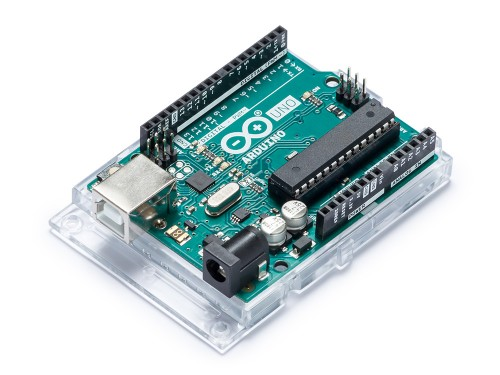
\includegraphics[width=2.5cm,valign=c]{Arduino_uno.jpg}\\Arduino UNO\end{tabular} & \begin{tabular}[c]{@{}l@{}}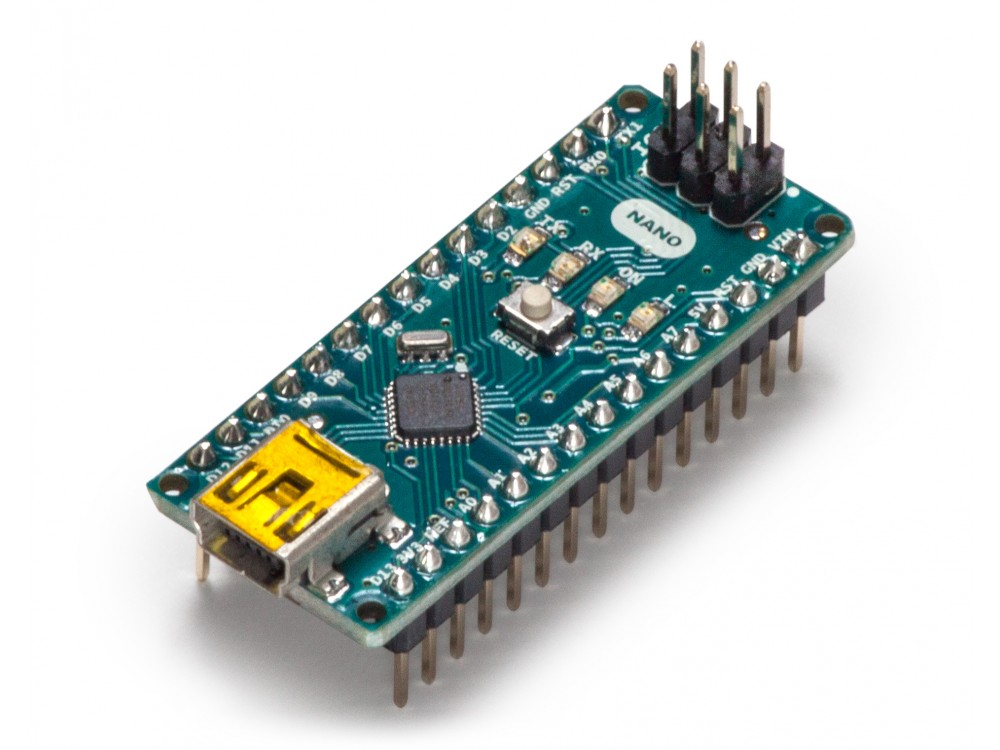
\includegraphics[width=2.5cm,valign=c]{arduino_nano.jpg}\\Arduino Nano\end{tabular} & \begin{tabular}[c]{@{}l@{}}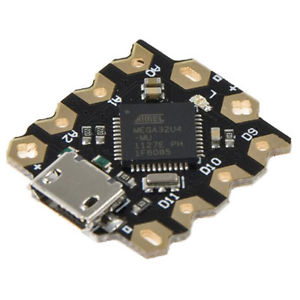
\includegraphics[width=2cm,valign=c]{beetle.jpg}\\Beetle\end{tabular}   & \begin{tabular}[c]{@{}l@{}}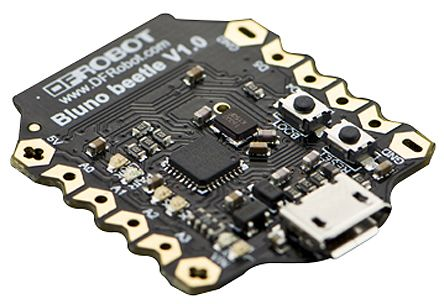
\includegraphics[width=2.5cm,valign=c]{bluno_beetle.jpg}\\Bluno Beetle\end{tabular} \\ \hline
		Sensor                    & \begin{tabular}[c]{@{}l@{}}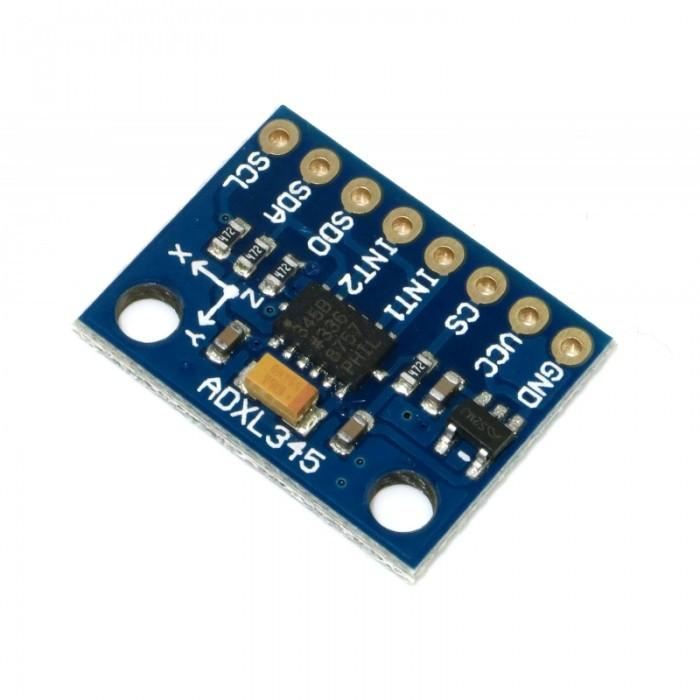
\includegraphics[width=2.2cm,valign=c]{ADXL345.jpg}\\ADXL345\end{tabular} & \begin{tabular}[c]{@{}l@{}}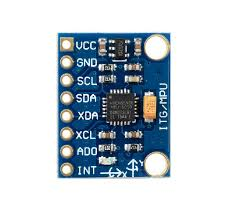
\includegraphics[width=2.4cm,valign=c]{mpu6050.jpg}\\MPU6050\end{tabular} & \begin{tabular}[c]{@{}l@{}}\\ \end{tabular} & \begin{tabular}[c]{@{}l@{}}\\ \end{tabular} \\ \hline
		Alignment mechanim        & \begin{tabular}[c]{@{}l@{}}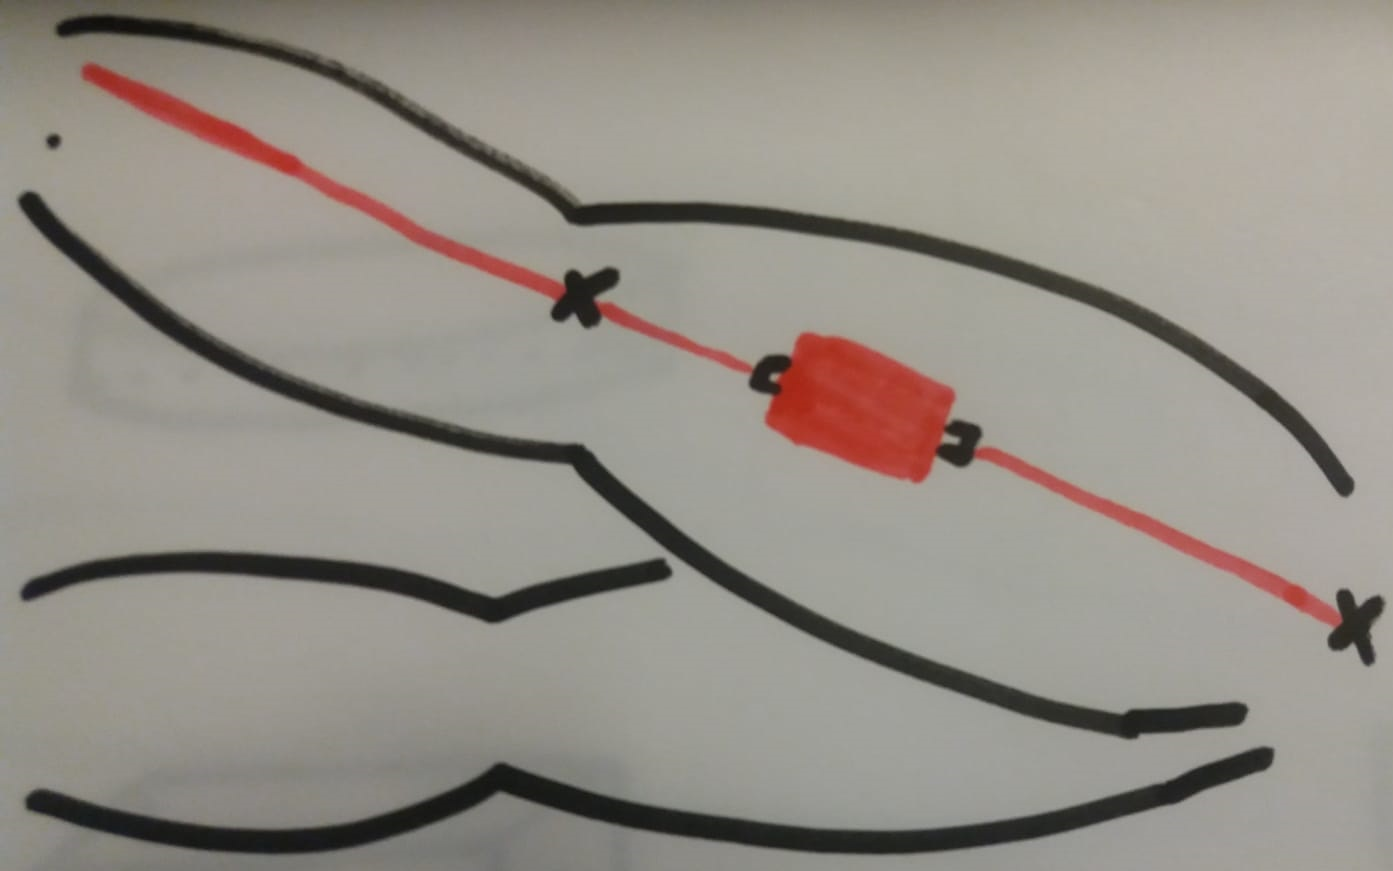
\includegraphics[width=2.5cm,valign=c]{concepts/laser_alignment.jpeg}\\laser alignment\end{tabular} & \begin{tabular}[c]{@{}l@{}}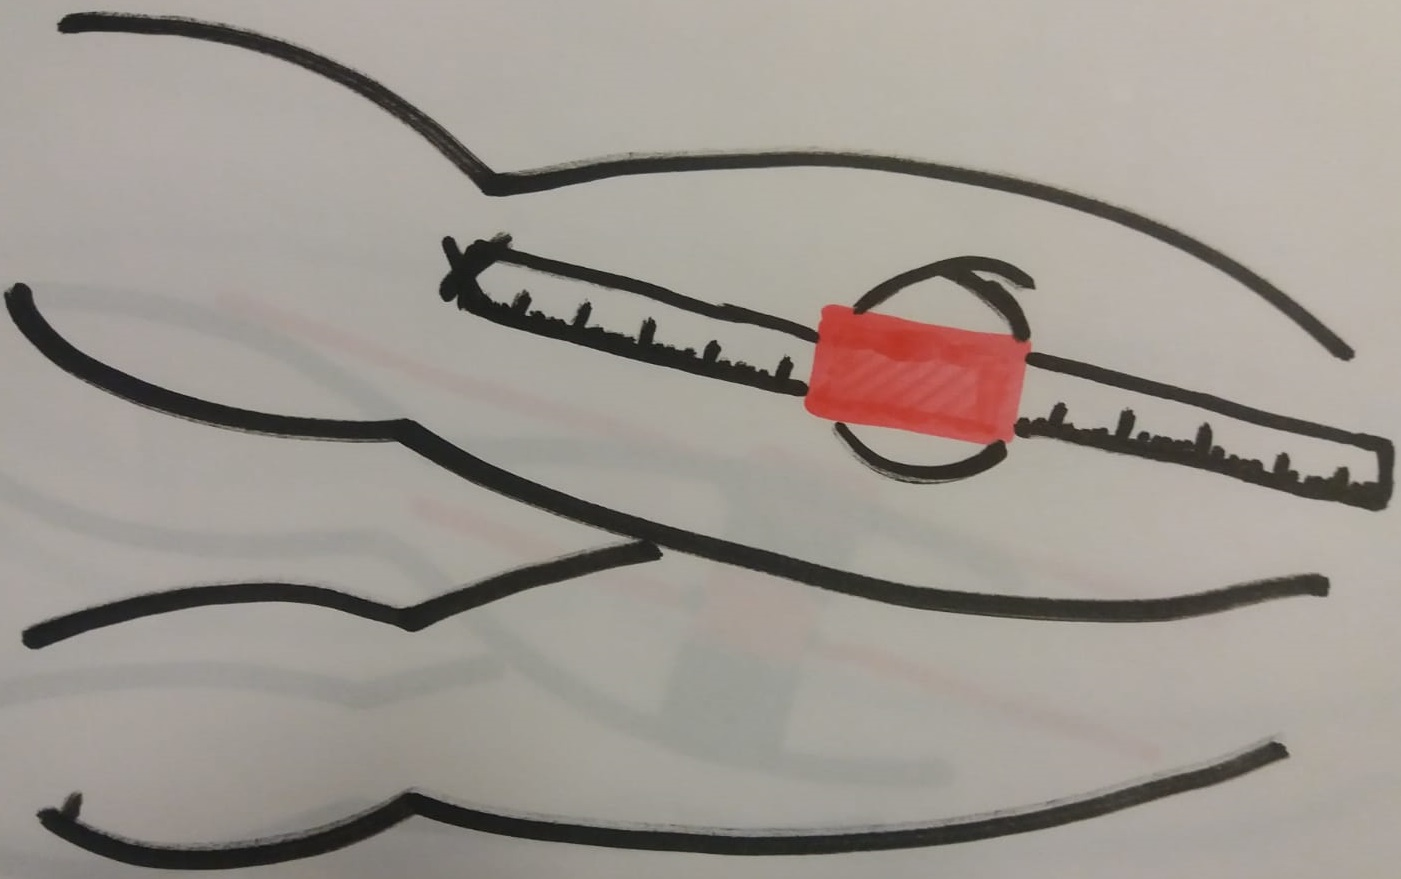
\includegraphics[width=2.5cm,valign=c]{concepts/ruler_alignment.jpeg}\\Ruler alignment\end{tabular} & \begin{tabular}[c]{@{}l@{}}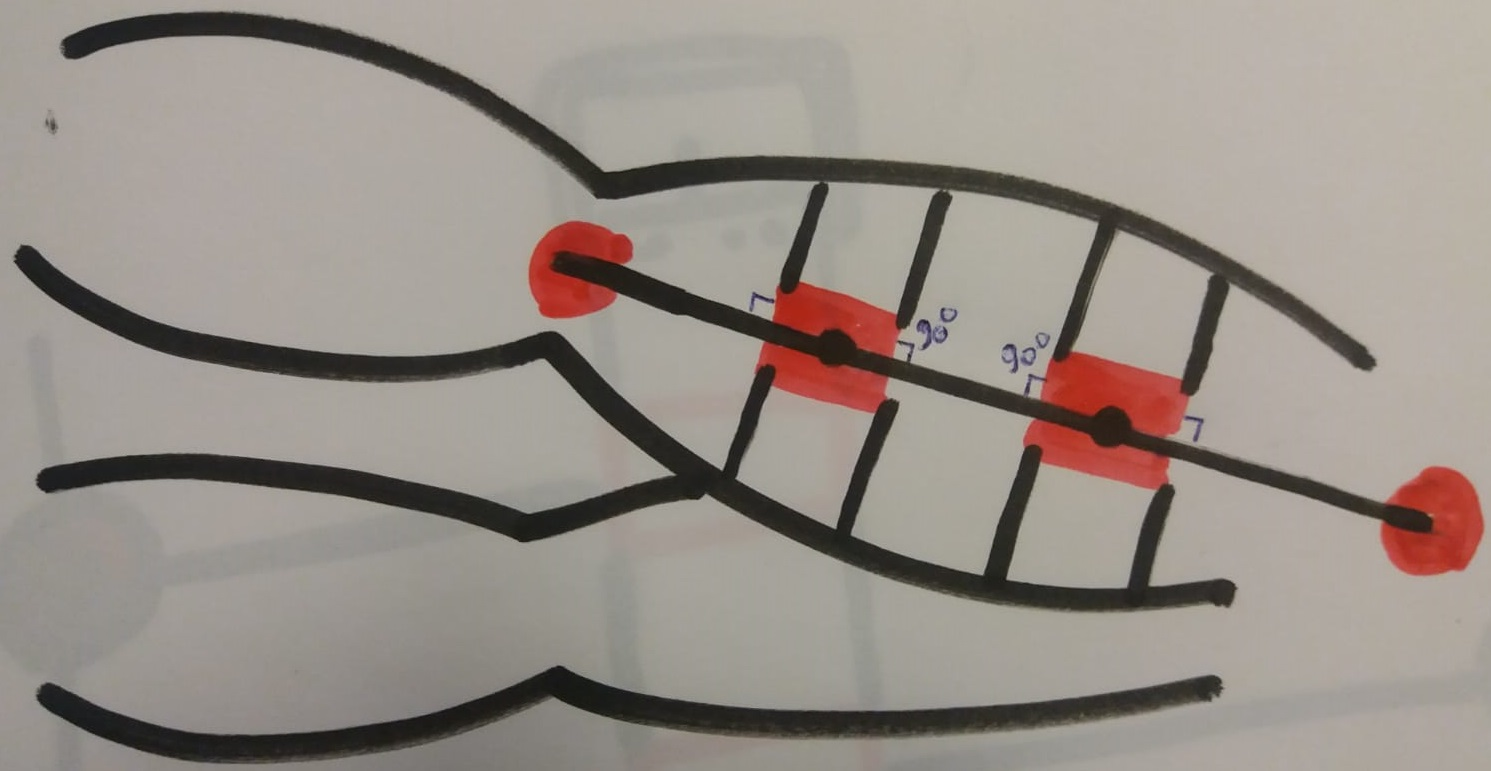
\includegraphics[width=2.5cm,valign=c]{concepts/IMU_combined_with_two_stickers_for_alignment.jpeg}\\stickers and \\elastic thread \end{tabular}   & \begin{tabular}[c]{@{}l@{}}\\ \end{tabular} \\ \hline
		Fixation placement        & \begin{tabular}[c]{@{}l@{}}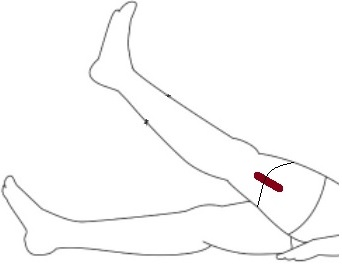
\includegraphics[width=2.5cm,valign=c]{fixation_leg1.jpg}\\Lateral part of\\the upper leg\end{tabular} & \begin{tabular}[c]{@{}l@{}}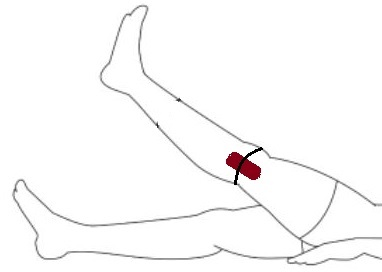
\includegraphics[width=2.5cm,valign=c]{knee_fixation2.jpg}\\lateral part\\of the knee\end{tabular} & \begin{tabular}[c]{@{}l@{}}\\\end{tabular}   & \begin{tabular}[c]{@{}l@{}}\\\end{tabular} \\ \hline
		Fixation method           & \begin{tabular}[c]{@{}l@{}}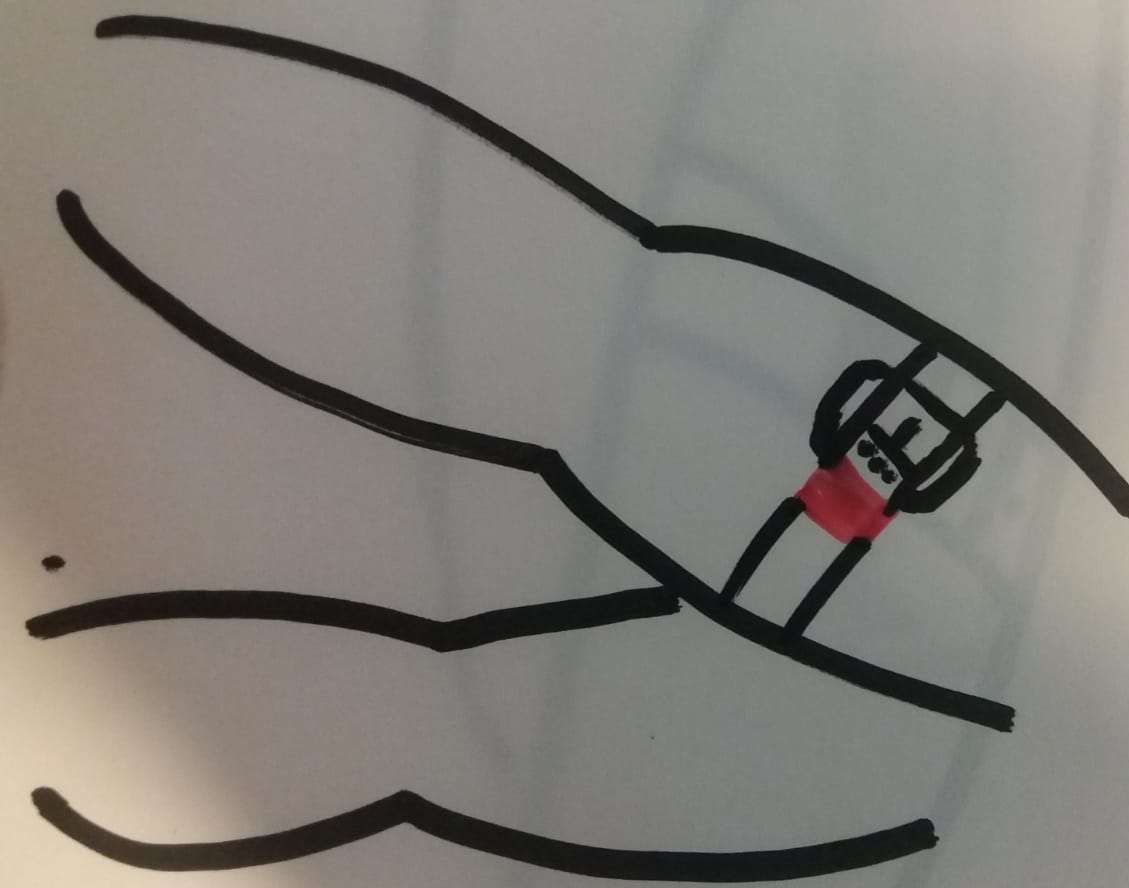
\includegraphics[width=2.5cm,valign=c]{concepts/belt.jpeg}\\Strap\end{tabular} & \begin{tabular}[c]{@{}l@{}}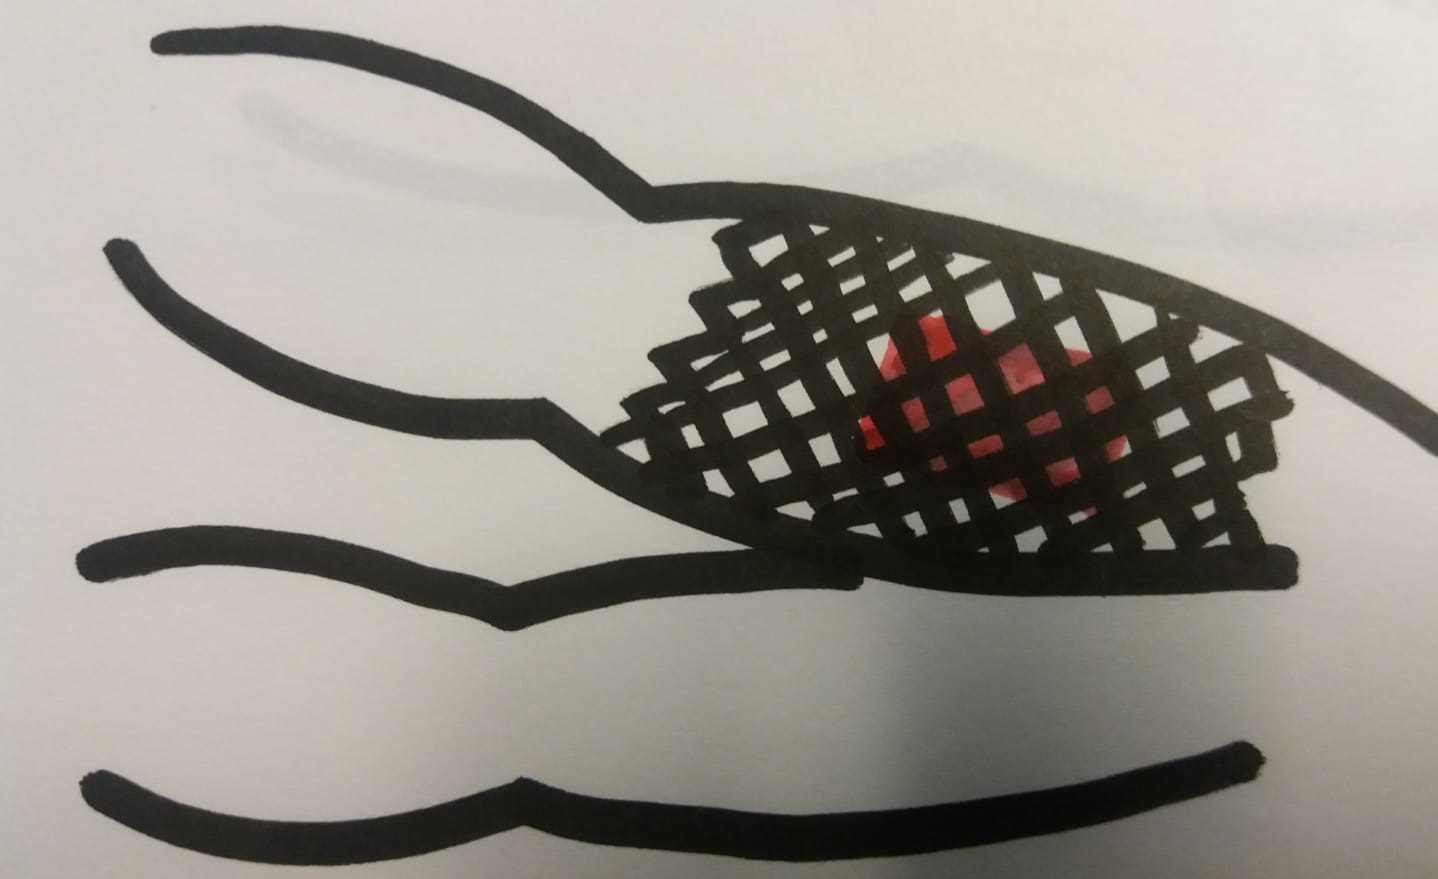
\includegraphics[width=2.5cm,valign=c]{concepts/gauze.jpeg}\\Gauze\end{tabular} & \begin{tabular}[c]{@{}l@{}}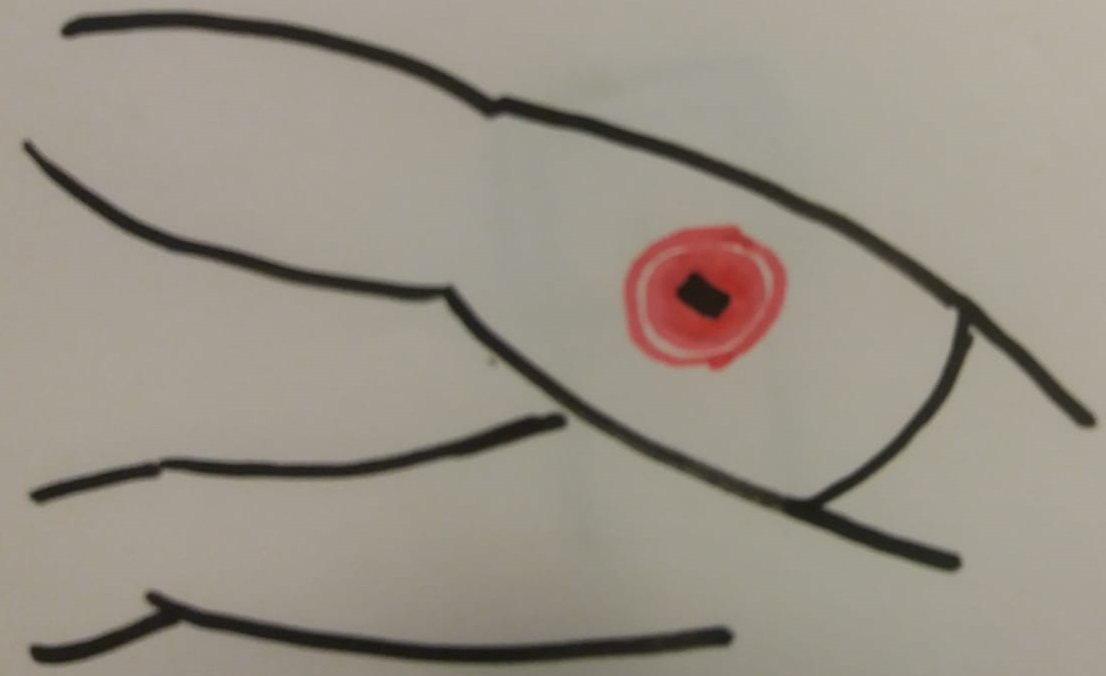
\includegraphics[width=2.5cm,valign=c]{concepts/sticker.jpeg}\\Sticker\end{tabular}   & \begin{tabular}[c]{@{}l@{}}\\ \end{tabular} \\ \hline
		Activation device         & \begin{tabular}[c]{@{}l@{}}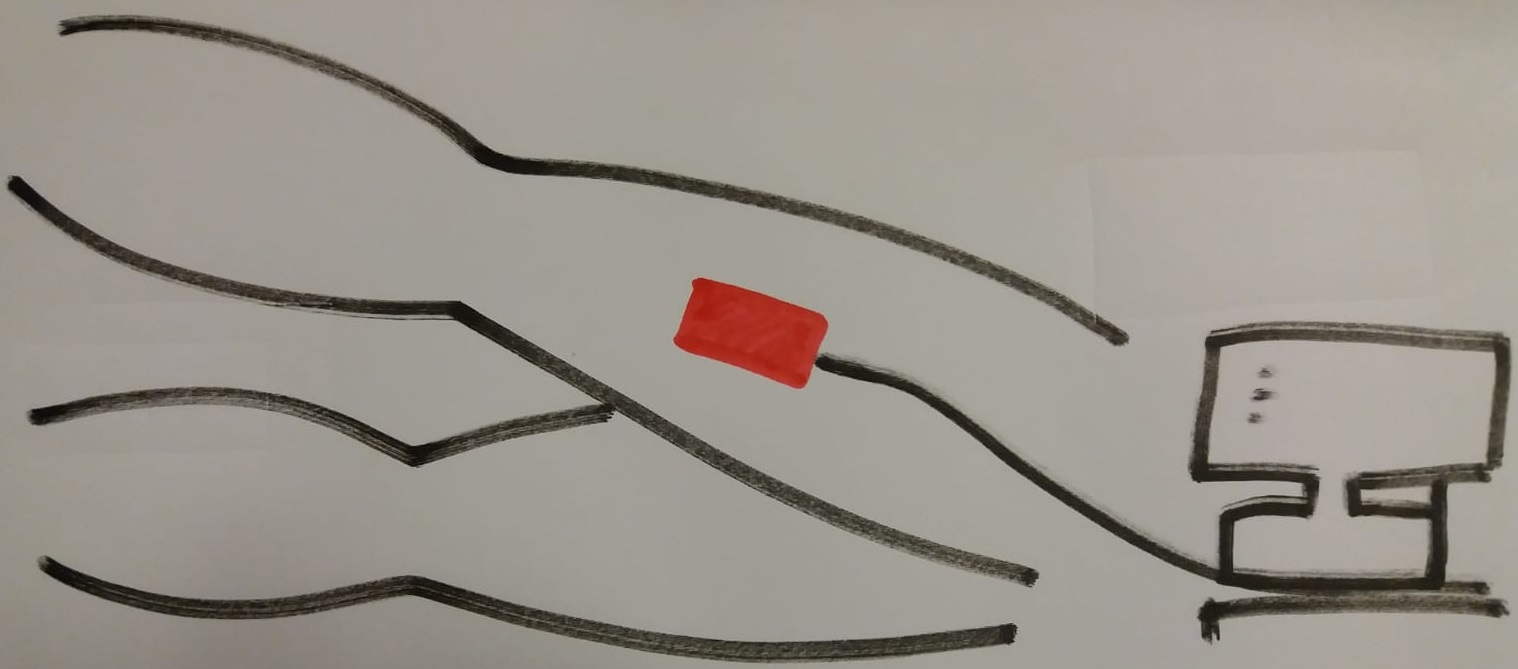
\includegraphics[width=2.5cm,valign=c]{activate_measurements_through_computer.jpg}\\ Operate device\\through computer\end{tabular} & \begin{tabular}[c]{@{}l@{}}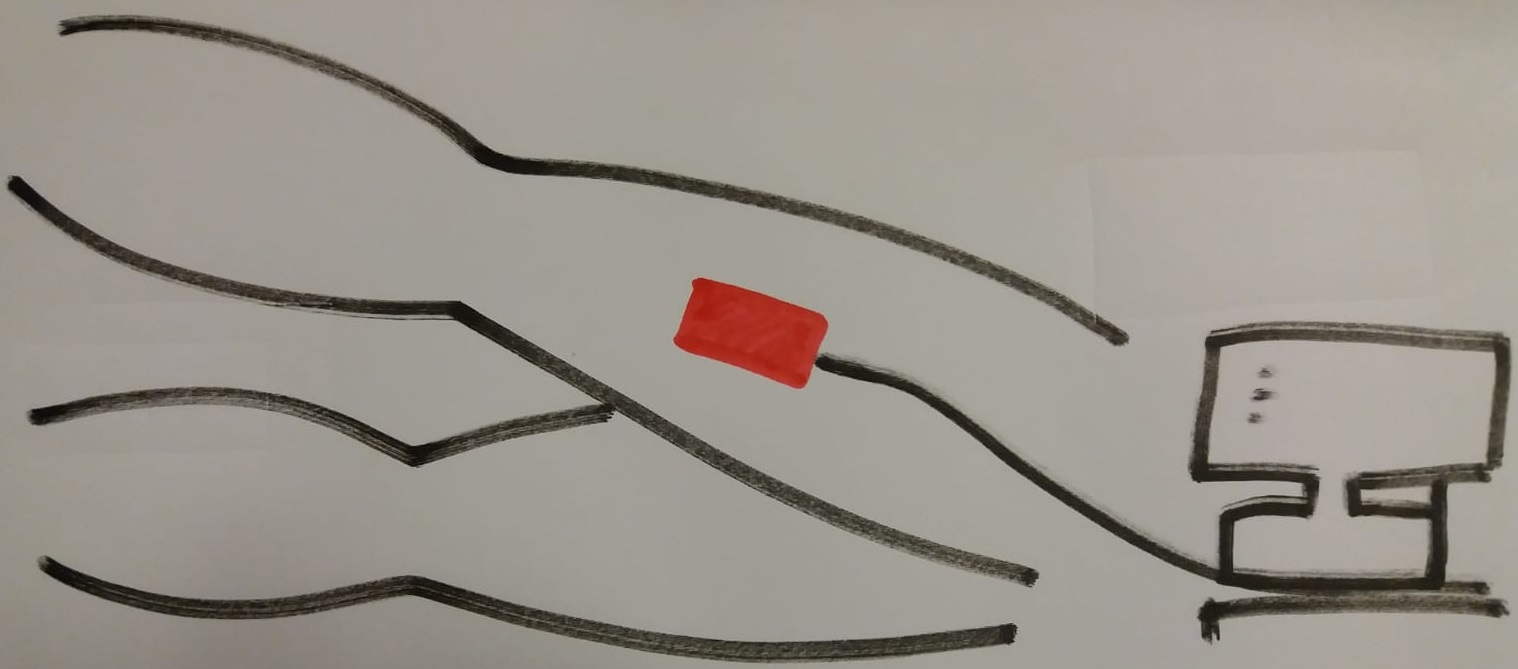
\includegraphics[width=2.5cm,valign=c]{button_on_leg.jpg}\\Activation device\\through button\end{tabular} & \begin{tabular}[c]{@{}l@{}}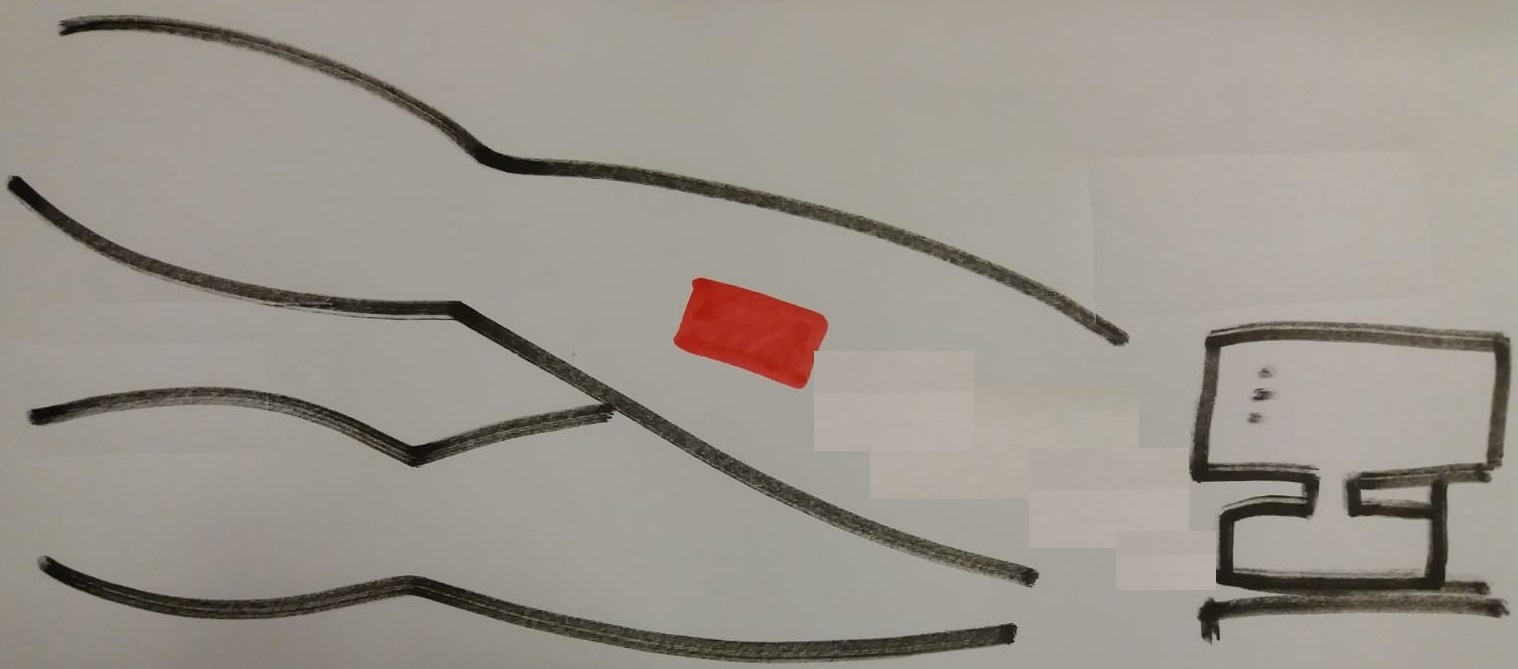
\includegraphics[width=2.5cm,valign=c]{activate_measurements_through_computer_wireless.jpg}\\Activation device\\through button \\wireless\end{tabular} & \begin{tabular}[c]{@{}l@{}}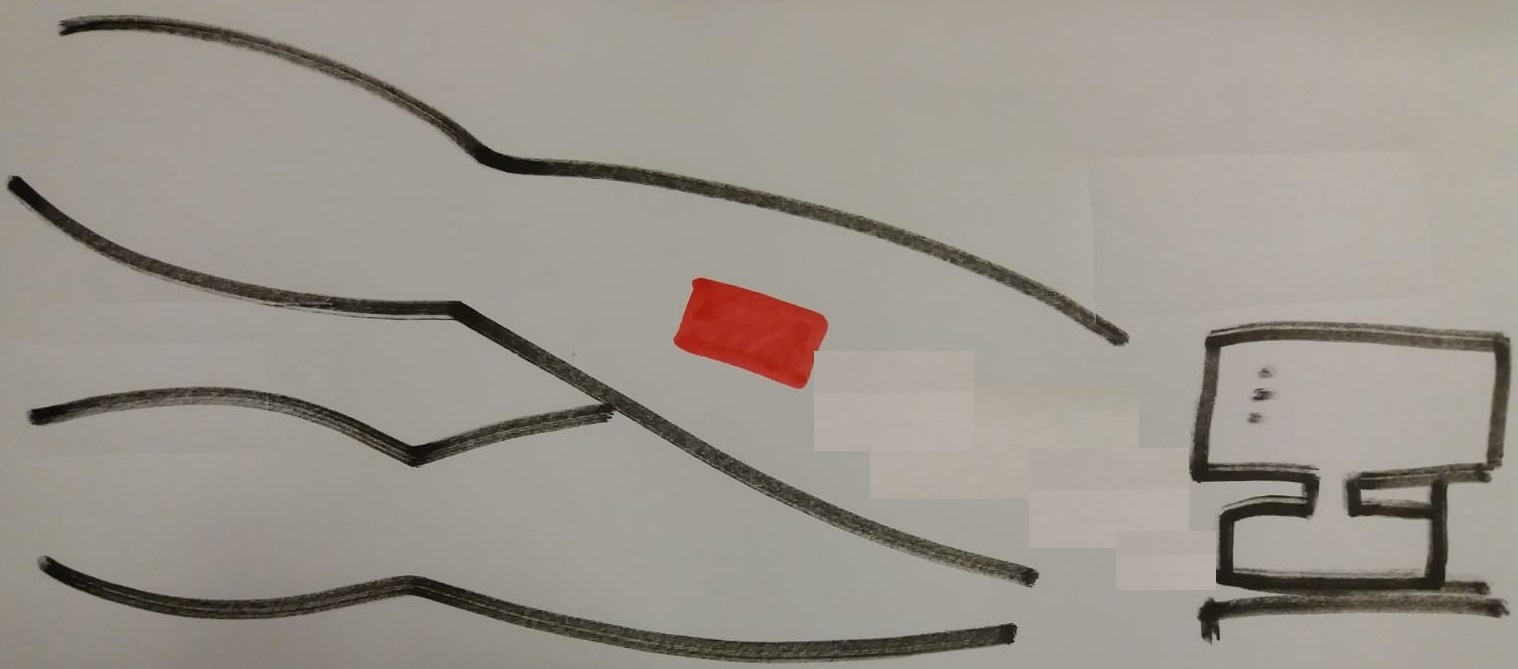
\includegraphics[width=2.5cm,valign=c]{activate_measurements_through_button_wireless.jpg}\\Activation device\\through computer\\wireless\end{tabular} \\ \hline
	\end{tabular}
\caption{The different concepts for each subfunction. The most promising ones will be used in the new solution}
\end{table}



\section{Microprocessor}
A commonly used microprocessor for making prototypes is the Arduino UNO. For initially testing the code I used this device. Next, to this sensor, three other sensors can be used, the Bluno Beetle, the Beetle and the Arduino Nano. These three microprocessors also use the Arduino Micro board, this makes it possible to directly use the same code that is written for the Arduino UNO. The  microprocessers, the MPU6050 and the ADXL345, both need to be connected to the data line (SDA) and the clock line (SCL) to communicate with the microprocessor(a more elaborate description about the communication can be read in chapter 4.5.2). All fourth microprocessors have a SCL and SDA output pin that can be used for this, so all the device can be used in combination with the IMU's. The device is easier to use by the orthopaedic if it is smaller, cause it will be easier to integrate it with a fixation element. The Beetle is the smallest of the devices(20mm x 22mm), the Arduino Nano is (43.18mm x 18.54mm), the Bluno Beetle (28.8mm x 33.1mm) and the Arduino UNO is (68.6mm x 53.3mm). The Bluno Beetle is bigger then the Beetle, however it allows for a wirelss bluetooth connection. A bluetooth connection could also be acclopmished by connecting a master and slave Bluetooth module. The combined microprocessor and the bluetooth would however result in a bigger circuit board then the Bluno Beetle. Because of the small size of the Beetle and the possibility for a bluetooth connection when using the Bluno Beetle, these two microprocessors appeared to be the best options. Both mircopocessors were selected for further evalatuation as it was not clear if the device would be wireless. The Harris profile (table 3.2) had the same outcome.
\begin{figure}[!htb]
	\centering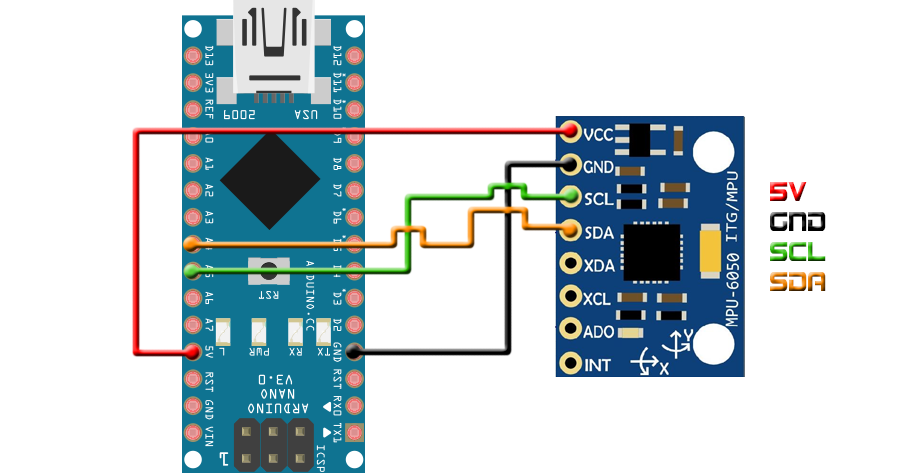
\includegraphics[width=260pt]{IMU_schematic.jpg}
	\caption{A schematic view of the MPU6050 sensor connected to the Arduino Nano~\cite{MPU6050connectedtoMicroprocessor}}
\end{figure}

\begin{table}[]
	\begin{tabular}{|l|l|l|l|l|l|l|l|l|l|}
		\hline
		\textbf{Microprocessor} & Weight    & \begin{tabular}[c]{@{}l@{}}The \\ Beetle\end{tabular} &       & \begin{tabular}[c]{@{}l@{}}Arduino \\ Nano\end{tabular} &       & \begin{tabular}[c]{@{}l@{}}Arduino \\ UNO\end{tabular} &       & \begin{tabular}[c]{@{}l@{}}Bluno \\ Beetle\end{tabular} &       \\ \hline
		\textit{Requirements}   & {[}1-3{]} & rating                                                & score & rating                                                  & score & rating                                                 & score & rating                                                  & score \\ \hline
		Safety                  & 3         & 4                                                     & 12    & 4                                                       & 12    & 4                                                      & 12    & 4                                                       & 12    \\ \hline
		Implementable           & 2         & 4                                                     & 8     & 3                                                       & 6     & 1                                                      & 2     & 4                                                       & 8     \\ \hline
		Usability               & 2         & 3                                                     & 6     & 3                                                       & 6     & 3                                                      & 6     & 4                                                       & 8     \\ \hline
		Complexity              & 2         & 4                                                     & 8     & 4                                                       & 8     & 4                                                      & 8     & 4                                                       & 8     \\ \hline
		Quality fixation        & 3         & 4                                                     & 12    & 3                                                       & 9     & 2                                                      & 6     & 4                                                       & 12     \\ \hline
		Feasilibity             & 2         & 3                                                     & 6     & 3                                                       & 6     & 3                                                      & 6     & 3                                                       & 6     \\ \hline
		Sterilisation           & 2         & 4                                                     & 8     & 4                                                       & 8     & 4                                                      & 8     & 4                                                       & 8     \\ \hline
		Proven concept          & 2         & 4                                                     & 8     & 2                                                       & 4     & 1                                                      & 2     & 4                                                       & 8     \\ \hline
		Total score             &           &                                                       & 68    &                                                         & 59    &                                                        & 50    &                                                         & 70    \\ \hline
	\end{tabular}
\caption{Harris profile for the different microprocessor. At the top, the different concepts are stated. On the left the different requirements with next to it the weight that is given to that requirement are listed. The bottom row shows the final score for each concept}
\label{table:draglift1}
\end{table}

\section{Sensor}
Two different IMU sensors were evaluated, the MPU6050 and the ADXL345 and one IMU combined with a magnetometer, the MPU9520. These three sensors are easy to obtain, affordable and widely used. Because these sensors are widely used multiple libraries can be found on the internet that can be direcltly be included in the code to provide a solid communication between the Arduino and the sensor. Because I did not have a background in programming, using these libraries was necessary. The MPU9520 combines a gyroscope, accelerometer and magnometer~\cite{infineon:MPU9520}. According to Dr. T. Horeman a magenometer could not be used because the device will be used in a hospital and most electrical devices contain components that interact with the magnetic field. This poses a problem when trying to precisely measure the earth magnetic field. The ADXL345 was recommended by Jos van Driel, the lab assistant in the meetshop. The MPU6050 was recommended when people asked a similar kind of question on te Arduio forum~\cite{Arduinoforum} or youtube~\cite{JoopBrokking}. The MPU6050 is an IMU that combines a 3-axis gyroscope and 3-axis accelerometer with an onboard Digital Motion Processor (DMP)~\cite{lucena2018mastication}\cite{infineon:MPU6050}. The DMP processes the complex 6-axis MotionFusion algorithms and can be used to process the raw data of the gyroscope and the accelerometer to usable angles. This sensor measures angular velocity and acceleration in translation direction in the three orthogonal directions. The ADXL345 is an accelerometer~\cite{infineon:ADXL345}. Because an accelerometer is not able to detect the yaw angle, a rotation around an axis that is aligned with the gravity vector, a gyroscope is needed to measure this angle. The gyroscope measurements around the roll and tilt angle can be corrected with the accelerometer measurements. For this reason, I choose the MPU6050. As it was clear that this is the better sensor no Harris profile is made for this part of the device.

\section{Alignment method}
The device needs to be aligned to appropriate skeletal landmarks that give information about the direction of the prosthetic. Important for this is that these landmarks can be identified and the device stays fixed in the right direction. The goniometer has a proximal arm that is aligned with the upper body and a distal arm that is aligned with the femur. The ROM is defined as the angle between these (figure 3.2). 
\begin{figure}[!htb]
	\centering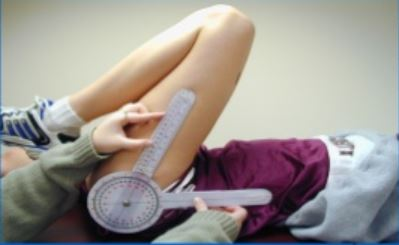
\includegraphics[width=200pt]{goniometer_measurement2.JPG}
	\caption{The distal arm is aligned with the femur and the proximal arm with the upperbody\cite{goniometer_measurement}}
\end{figure}

Other skeletal landmarks that can be used are the greater trochanter and the lateral epicondyle of the femur. A straight line drawn from both landmarks is similar to the orientation of the prosthetic. The orientation of the pelvis can be determined by measuring the direction of the femur when the patients have its legs flat on the table. This orientation is similar to the pelvic orientation which can be used as a reference line. A downside of using the femur as a skeletal landmark is that it can be hard to identify the exact orientation for larger build legs as the distance between the skin and the femur is too large. The lateral epicondyle and greater trochanter of the femur, on the other hand, are more easy to identify as they lay more superficial. The best option is to use all three skeletal landmarks.
\newline
\newline
Three different solutions are stated to align the device with the skeletal landmarks. Alignment through a line laser, a ruler and a sticker that can be attached on lateral epicondyle and the greater trochanter (see figure 3.3 and 3.4). When using the laser a light beam is shone in a straight line on the lateral side of the leg. The light should cross the lateral epicondyle of the femur and the greater trochanter. If this is the case the device can be fixed while the beam is still crossing these landmarks. A goniometer can also be used to align the device. The stationary arm should cross the lateral epicondyle and the movable arm should cross the greater trochanter. If this is the case the device can be fixed. After this, the movable arm can be folded back so the area around the hip joint is free. Another option is to use two stickers where one is placed on the lateral epicondyle and one the greater trochanter. An elastic thread connects the device on the leg with the sticker on the knee and the hip. The device will be 'pulled' in the right orientation by the elastic threads. The thread and sticker on the hip can be removed when the device is aligned with the prosthetic. The device stays in the right orientation because of the elastic wire that is connected to the sticker on the lateral epicondyle of the femur. The Harris profile showed that the laser beam is the best option (table 3.3). Because the device does is smaller (it does not have extended parts like the ruler or the wires) it requires less space when it is attached on the leg. It easier to implement this device in the current procedure as it will not limit the workspace of the orthopeadic surgeon.
\begin{figure}[!htb]
	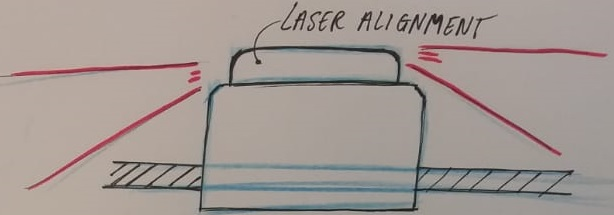
\includegraphics[width=0.5\linewidth]{laser_alignment.jpg}
	\caption{The device is fixed with a strap on the upperleg. A movable ruler is used to align the device with the lateral epicondyle and the greater trochanter.}
	\label{fig:my_label}
\end{figure}
\begin{figure}[!htb]
	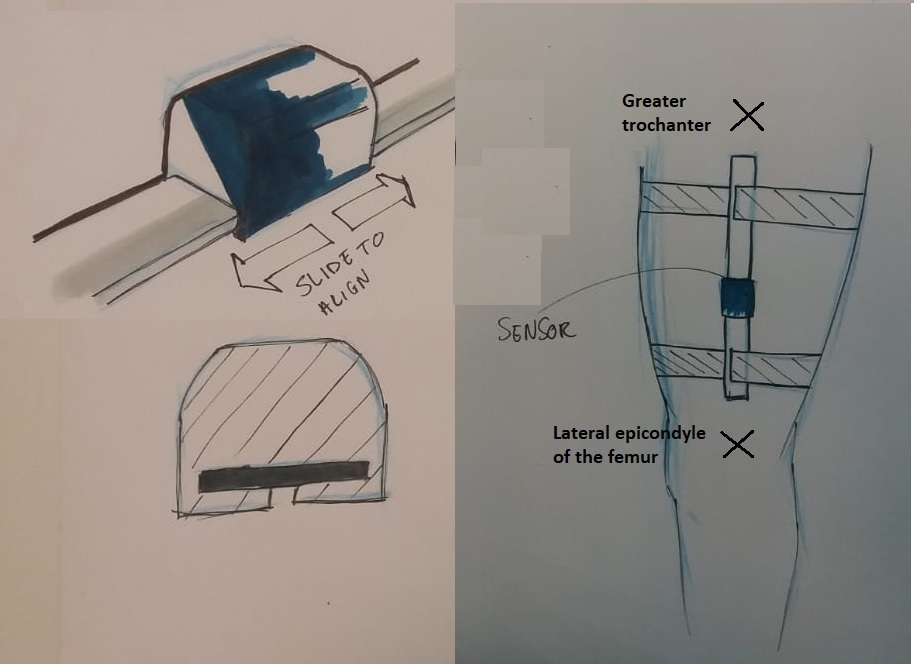
\includegraphics[width=1\linewidth]{ruler_alignment2.jpg}
	\caption{A movable ruler is used to align the device with the lateral epicondyle and the greater trochanter.}
	\label{fig:my_label}
\end{figure}

%\textbf{}laser too big
\begin{table}[t!]
	\begin{tabular}{|ll|ll|ll|ll|}
		\hline
		\multicolumn{1}{|l|}{\textbf{Alignment mechanism}}     & Weight    & Laser                       &       & Ruler                       &       & Elastic thread              &       \\ \cline{1-1}
		\multicolumn{1}{|l|}{\textit{Requirements}} & {[}1-3{]} & \multicolumn{1}{l|}{rating} & score & \multicolumn{1}{l|}{rating} & score & \multicolumn{1}{l|}{rating} & score \\ \hline
		\multicolumn{1}{|l|}{Safety}                & 3         & \multicolumn{1}{l|}{5}      & 15    & \multicolumn{1}{l|}{5}      & 15    & \multicolumn{1}{l|}{5}      & 15    \\ \hline
		\multicolumn{1}{|l|}{Implementable}         & 2         & \multicolumn{1}{l|}{5}      & 10    & \multicolumn{1}{l|}{3}      & 6     & \multicolumn{1}{l|}{3}      & 6     \\ \hline
		\multicolumn{1}{|l|}{Usability}             & 2         & \multicolumn{1}{l|}{3}      & 6     & \multicolumn{1}{l|}{2}      & 4     & \multicolumn{1}{l|}{1}      & 2     \\ \hline
		\multicolumn{1}{|l|}{Complexity}            & 2         & \multicolumn{1}{l|}{4}      & 8     & \multicolumn{1}{l|}{4}      & 8     & \multicolumn{1}{l|}{4}      & 8     \\ \hline
		\multicolumn{1}{|l|}{Quality alignment}     & 3         & \multicolumn{1}{l|}{3}      & 9     & \multicolumn{1}{l|}{3}      & 9     & \multicolumn{1}{l|}{4}      & 12    \\ \hline
		\multicolumn{1}{|l|}{Feasibility}           & 2         & \multicolumn{1}{l|}{3}      & 6     & \multicolumn{1}{l|}{3}      & 6     & \multicolumn{1}{l|}{3}      & 9     \\ \hline
		\multicolumn{1}{|l|}{Sterilisation}         & 2         & \multicolumn{1}{l|}{3}      & 6     & \multicolumn{1}{l|}{3}      & 6     & \multicolumn{1}{l|}{3}      & 6     \\ \hline
		\textbf{Total score}                        &           &      60                       &       &         54                    &       &                             &     57  \\ \hline
	\end{tabular}
	\caption{Harris profile of the concepts for the alignment mechanism. At the top, the different concepts are stated. On the left the different requirements with next to it the weight that is given to that requirement are listed. The bottom row shows the final score for each concept}
	\label{table:draglift1}
\end{table}

\section{Fixation placement}
To align the device with the skeletal landmarks it needs to move in the same motion as the prosthesis. To achieve this the device needs to be connected on a position where it stays aligned with the skeletal landmarks. The device can be fixed on the lateral or anterior part of the upper leg or knee. Tests were performed by connecting straps to the knee to evaluate if the skin deforms one of these spots, if this happens the lower leg would influence the orientation of the device which gives an error in the measurement (see figure 3.5). The following strap was connected to the knee while the upper leg fixed. The orientation of the device did not stay aligned with the prosthesis, when the knee was bent. The same change in direction is also expected when the device is connected with a gauze or a sticker.
\begin{figure}[!htb]
	\centering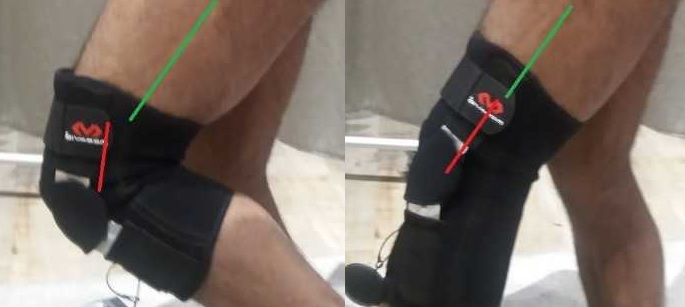
\includegraphics[width=450pt]{orientation_knee_device2.jpg}
	\caption{A commercial strap was connected to my knee to evaluate if the direction of the red line is changed when the knee is extended. It is seen that the red line is not in l}
\end{figure}

\section{Fixation method}
The three methods to connect the device are the usage of straps, gauze/sleeves and a sticker. Straps are normally used to fasten or bind items(figure 3.6). The tighter the strap is, the less likely it moves to a different position. If the upper leg has a lot of loose skin tissue it may be hard to fix the device in one position. The position of the skin in relation to the bone also changed when the strap is attached. 
% HIER MORGEN VERDER WERKEN.. DUBBELE INFO MET FIXATION PLACEMENT
Sleeves can also be used, an advantage here is that the material of the sleeve is flexible and adapts to the build of the leg. The tightness of the sleeve depends on the circumference of the leg, if this is too small the device moves from its initial position. If the circumference is too big it may not be possible to fix the sleeve. When the sleeve is connected to the knee it is expected that the sleeve also bends when the knee is bent. This will changes its orientation relative to prosthetic. Another option is the usage of a sticker. The sticker is directly attached to the skin of the leg. When the sticker is used the skin is not deformed, however, if the skin is attached to the upper leg and the skin is not very tight it may change its position relative to the femur when the leg is lifted from the table. If the sticker is attached to the lateral side of the knee it is also expected that the orientation will change relative to the prosthetic due to stretching of the skin. In table 3.4 the three different concepts are scored in a Harris profile. Because the sticker can not be sterilised and misalignment can occur due to soft tissue artefacts\cite{kratzenstein2012effective} the sticker is not a suitable option. The strap is also more feasible to be fixed on different bodybuilds of the leg compared to the sleeve. Because of this the strap seems to be the most promising solution. 
\begin{table}[!tbh]
	\begin{tabular}{|ll|ll|ll|ll|}
		\hline
		\multicolumn{1}{|l|}{\textbf{Fixation method}}     & Weight    & Sticker                       &       & Gauge/Sleeve                       &       & Strap              &       \\ \cline{1-1}
		\multicolumn{1}{|l|}{\textit{Requirements}} & {[}1-3{]} & \multicolumn{1}{l|}{rating} & score & \multicolumn{1}{l|}{rating} & score & \multicolumn{1}{l|}{rating} & score \\ \hline
		\multicolumn{1}{|l|}{Safety}                & 3         & \multicolumn{1}{l|}{4}      & 12    & \multicolumn{1}{l|}{4}      & 12    & \multicolumn{1}{l|}{4}      & 12    \\ \hline
		\multicolumn{1}{|l|}{Implementable}         & 2         & \multicolumn{1}{l|}{4}      & 8     & \multicolumn{1}{l|}{4}      & 8     & \multicolumn{1}{l|}{4}      & 8     \\ \hline
		\multicolumn{1}{|l|}{Usability}             & 2         & \multicolumn{1}{l|}{3}      & 6     & \multicolumn{1}{l|}{2}      & 4     & \multicolumn{1}{l|}{3}      & 6     \\ \hline
		\multicolumn{1}{|l|}{Complexity}            & 2         & \multicolumn{1}{l|}{4}      & 8     & \multicolumn{1}{l|}{4}      & 8     & \multicolumn{1}{l|}{4}      & 8     \\ \hline
		\multicolumn{1}{|l|}{Quality alignment}     & 3         & \multicolumn{1}{l|}{2}      & 6     & \multicolumn{1}{l|}{4}     & 12     & \multicolumn{1}{l|}{4}      & 12    \\ \hline
		\multicolumn{1}{|l|}{Feasibility}           & 2         & \multicolumn{1}{l|}{3}      & 6     & \multicolumn{1}{l|}{2}      & 4     & \multicolumn{1}{l|}{3}      & 6     \\ \hline
		\multicolumn{1}{|l|}{Sterilisation}         & 2         & \multicolumn{1}{l|}{2}      & 6     & \multicolumn{1}{l|}{4}      & 8     & \multicolumn{1}{l|}{4}      & 8     \\ \hline
		\textbf{Total score}                        &           &      52                       &       &         56                    &       &                             &     60  \\ \hline
	\end{tabular}
	\caption{Harris profile of the concepts for the fixation method. At the top, the different concepts are stated. On the left the different requirements with next to it the weight that is given to that requirement are listed. The bottom row shows the final score for each concept}
	\label{table:draglift1}
\end{table}
\begin{figure}[!htb]
	\includegraphics[width=1\linewidth]{strap_sketch.jpg}
	\caption{A sketch of the strap is used to connect the sensor on the leg.}
	\label{fig:my_label}
\end{figure}

\section{Activation device}
The device can be connected to a laptop via Bluetooth with an USB cable. To test the wireless system two Bluno Beetles were used. One Bluno Beetle was connected to the computer with a USB cable and another one connected to a external powersupply and the MPU6050 (see figure 3.7). The Bluno beetle connected to the computer was configured to receive data and the other microprocessor was configured to send data. The Serial monitor of the Arduino software showed that measurements of the MPU6050 were send to the computer. A problem that may occur wen using an external powersupply is the sterilisation of the device. The batteries should be disconnected if the device is sterilised under high pressure or high temperature. The downside of a cable however is that it may hinder the surgical team in moving freely through the operation room. 
\begin{figure}[!htb]
	\centering\includegraphics[width=170pt]{bluetooth_bluno_beetle.jpeg}
	\caption{The Bluno Beetle is held in my hand and the MPU650 connected on the breadboard is moved, the Bluno Beetle lying on the table detects the measurement and the Serial monitor of the Arduino displays the measurements.}
\end{figure} 
\newline
\newline
To activate the device, it can be operated through the computer or via a button on the device. If the device is operated through a button the surgical drape should be removed to press the button or the button is operable under the drape. Because the surgeon already needs to pay attention to the computer to read the different ROM values for the different axes and the device will be covered by the surgical drape it may be easier to operate the device from the computer. All options have there benefits and drawbacks. If the sterilisation problem for the batteries is solved then the best option would be a wireless device operated through the computer or a button. The score of the different concepts can bee seen in table 3.5.

\begin{table}[!tbh]
	\begin{tabular}{|l|l|l|l|l|l|l|l|l|l|}
		\hline
		\textbf{Microprocessor} & Weight    & \begin{tabular}[c]{@{}l@{}}USB+\\Button \end{tabular}&       & \begin{tabular}[c]{@{}l@{}}USB+\\computer\end{tabular} &       & \begin{tabular}[c]{@{}l@{}}Wireless+\\Button\end{tabular} &       & \begin{tabular}[c]{@{}l@{}}Wireless+\\Computer\end{tabular} &       \\ \hline
		\textit{Requirements}   & {[}1-3{]} & rating                                                & score & rating                                                  & score & rating                                                 & score & rating                                                  & score \\ \hline
		Safety                  & 3         & 4                                                     & 12    & 4                                                       & 12    & 4                                                      & 12    & 4                                                       & 12    \\ \hline
		Implementable           & 2         & 3                                                     & 6     & 4                                                       & 8     & 3                                                      & 6    & 4                                                       & 8     \\ \hline
		Usability               & 2         & 3                                                     & 6     & 4                                                       & 8     & 3                                                      & 6    & 4                                                       & 8     \\ \hline
		Complexity              & 2         & 4                                                     & 8     & 4                                                       & 8     & 4                                                      & 8     & 4                                                       & 8     \\ \hline
		Quality fixation        & 3         & 3                                                     & 9    & 3                                                       & 9     & 4                                                      & 12     & 4                                                       & 12     \\ \hline
		Feasilibity             & 2         & 3                                                     & 6     & 3                                                       & 6     & 3                                                      & 6     & 3                                                       & 6     \\ \hline
		Sterilisation           & 2         & 4                                                     & 8     & 4                                                       & 8     & 2                                                      & 4     & 2                                                       & 4     \\ \hline
		Total score             &           &                                                       & 55    &                                                         & 59    &                                                        & 54    &                                                         & 58    \\ \hline
	\end{tabular}
	\caption{Harris profile for the different methods for operating the device. At the top, the different concepts are stated. On the left the different requirements with next to it the weight that is given to that requirement are listed. The bottom row shows the final score for each concept}
	\label{table:draglift1}
\end{table}

\section{Conclusions}
The most promising concepts of every subfunction are summarized in this chapter. 
\newline
\newline
\textbf{Microprocessor} \newline
The Bluno Beetle sensor is chosen as the most promising concept because it is small which allows for better fixation and alignment with the skeletal landmarks and it allows for Bluetooth connection.  \newline
\newline
\textbf{IMU} \newline
The MPU6050 is chosen because it is affordable, it is more commonly used compared to other IMU's which makes writing the code and debugging it easier and it combines a gyroscope and accelerometer. 
\newline
\newline
\textbf{Alignment method} \newline
The laser seems to be the most promising solution. The precision of the alignment of the elastic thread may be better as the device is pulled in the correct orientation by the thread connected on the landmarks, however the area covered by the device is much bigger as there is sticker on the knee and a thread. It also may be hard to prevent that the elastic thread does not loosen or dettach. The surgical staff has to pay extra attention to this which affects the usability of the device. 
\newline
\newline
\textbf{Fixation placement} \newline
Because it is very difficult to keep the device aligned with the prosthetic when it is placed on the knee, the upper leg is chosen.  
\newline 
\newline
\textbf{Fixation method} \newline
The most promising fixation method is the usage of straps. This is because it can be reused and sterilised in contrast to the sticker and it allows for a strong fixation for a large range of leg builds. The next chapter will further elaborate on the exact design and material of the strap. 
\newline
\newline
\textbf{Activation device} \newline
For this thesis the most feasible option will be used, operate the device via the computer where a USB cable connects it. All options have there benefits and drawbacks, however the feasibility of the button and bluetooth is already shown in this chapter and will not be elaborated on in the next chapters. The reason is that problems regarding failure of the button or bluetooth can lead to incorrect results during the tests. Additonally the sterilisation of the batteries also needs to be solved.  


{\chapter{Device manufacturing} 
In this chapter the different chosen concepts for each subfunction are further developed into real solutions and combined in a final design. This chapter consists of two parts. In the first part the different sub-parts will be shown leading to the final assembly. In the second part the calculations of the raw values to ROM values will be explained, the calibration method for the MPU6050 and the compensation for the drift of the gyroscope.  
%\section{subparts\&assembly}
\section{Electronics}
For the electronical part two different microprocessor can be used, the Beetle (figure 4.1a) and the Bluno Beetle (figure 4.1b). The Beetle is the smallest arduino based microprocessor.

\begin{figure}[H]
	\centering
\begin{subfigure}[b]{0.5\linewidth}
			\centering\includegraphics[width=200pt]{mpu6050_with_beetle.jpg}
			\caption{\label{fig:fig1}}
		\end{subfigure}%
	\begin{subfigure}[b]{0.5\linewidth}
		\centering\includegraphics[width=200pt]{laser_combined_with_microprocessor.jpg}
		\caption{\label{fig:fig2}}
	\end{subfigure}
	\caption{\subref{fig:fig1} shows the MPU6050 connnected with the beetle~\subref{fig:fig2} shows the MPU6050 connected with the Bluno Beetle and two line lasers}
\end{figure}

Because the option to use Bluetooth on the device is important the Bluno Beetle was chosen as the best device. However as stated in chapter 3.9 a cable will be used to connect the Bluno Beetle to the computer. The reason is that problems regarding failure of the bluetooth can lead to incorrect experimental results, additionally the sterilisation of the batteries is a problem. To avoid these two issues the prototype in this report will use a cable. The two line lasers, the LFL650-5-12, were connected to the device (figure 4.2). These two line laser are low-cost and belong to the laser class 1 which means that they are not harmful for the eye. They have an uniform line thickness and operate between 3-12V. This voltage output can be supplied by the Bluno Beetle.
\begin{figure}[htb]
	\centering\includegraphics[width=300pt]{casing/line_laser.jpg}
	\caption{The line laser used.}
\end{figure}
\section{Strap}
The strap that is made can be seen in figure 4.3. It can be connected on the upper leg (figure 4.4). The strap uses a belt and a velcro strap to fix it around the leg. The strap is made of 80\% polyester and 20\% spandex and viscose where a velcro was sewed on the strap.

\begin{figure}[htb]
	\centering\includegraphics[width=460pt]{strapv2.jpg}
	\caption{The strap that is used to evaluate can be seen in the figure. The strap can be streched at the areas marked with the orange box. This strapped allows for fixation of the strap for different bodybuilds.}
\end{figure}
\begin{figure}[H]
	\centering\includegraphics[width=460pt]{strapv2_on_leg.jpeg}
	\caption{The strap is connected on the right leg.}
\end{figure}
\section{Casing}
The casing should allow for protection of the electronics and make sufficient contact with the strap. The strap and casing can be integrated in one design or used as two tools. The choice is made to have the casing as a seperate tool. If they are seperate the device will be concected by a velcro on the strap. The advantage is that when the device is be placed in the right orientation the position of the strap doesnt have to be changed. It is easier to move the device than the whole strap.
\newline
\newline
The casings are designed are made by a Computer-aided design (CAD) program Solidworks® 2018 and 3D printed with the Ultimaker 2+ extended. The first design can be seen in figure 4.5a&b. It is box with a mold that can hold the microprocessor. The mold has the same dimensions as the Bluno Beetle. The design also has two holes for the lasers and one for the USB cable. The laser holes have the same diameter of the lasers. The friction force between the holes and the lasers make sure they stay fixed in the right position.  
\newline
A drawback of this design was that the MPU6050 was not fixed in the casing. This can lead to incorrect measurements if the movement of the sensor is caused by something else than the hip joint. The sensor also moved from it's position when the casing was potted with Epoxacast (figure 4.7). Additionally this design did not make enough contact with the strap to ensure it would stay fixed in the same position.
\begin{figure}[htb]
	\centering
	\begin{subfigure}{0.45\linewidth}
		\centering\includegraphics[width=140pt]{casing/bluno_beetle_casing_v6_without_laser_holder.JPG}
		\caption{\label{fig:fig1}}
	\end{subfigure}%
	\begin{subfigure}{0.45\linewidth}
		\centering\includegraphics[width=140pt]{casing/casing_box_front.jpeg}
		\caption{\label{fig:fig2}}
	\end{subfigure}  
	\caption{\subref{fig:fig1} shows the casing CAD drawing and~\subref{fig:fig2} the 3D printed casing.}
\end{figure}

The choice was made to increase the width of the casing to increase the contactpoints between the casing and the strap (figure 4.6a\&c). Additionally a laser holder was added to the casing (figure 4.6b&d).

\begin{figure}[H]
	\centering
	\begin{subfigure}{0.4\linewidth}
		\centering\includegraphics[width=140pt]{casing/bluno_beetle_casing_v8_round_design.JPG}
		\caption{\label{fig:fig1}}
	\end{subfigure}%
	\begin{subfigure}{0.4\linewidth}
		\centering\includegraphics[width=140pt]{casing/laser_holder.JPG}
		\caption{\label{fig:fig2}}
	\end{subfigure}  
	\begin{subfigure}{0.4\linewidth}
		\centering\includegraphics[width=140pt]{casing/bluno_beetle_casing_v8_round_design_picture.jpeg}
		\caption{\label{fig:fig3}}
	\end{subfigure}  
	\begin{subfigure}{0.4\linewidth}
	\centering\includegraphics[width=140pt]{casing/MU6050_with_laser_holder.jpg}
	\caption{\label{fig:fig4}}
	\end{subfigure}  
	\caption{26\subref{fig:fig1} shows the round casing. The laser holder is placed in a casing and the two holes of the MPU6050 are pushed over the two cilinders~\subref{fig:fig2}. The friction force between the two cilindrical extrusions and the two holes fixes the MPU6050. \subref{fig:fig3} shows the 3D printed casing and \subref{fig:fig4} the MPU6050 with the laser holder.}
\end{figure}

The point to surface contact was further increased by applying a surface curvature (figure 26).

\begin{figure[H]
	\centering\includegraphics[width=1\linewidth]{casing/Casing_with_curvature_picture.jpeg}
	\caption{The casing from figure 26 is compared with the two new designs. The curvature of the casing in the middle was too large. The casing in the right of the picture has a smaller curvature. This allowed the best fixation on the strap.}
\end{figure}

\section{Sterilisation}
The design of the device should allow protection and sterilisation of the device. Different sterilisation were described in chapter 2.10. The most commonly used technique, saturated steam, is not applicable for the inertial measurement unit and microprocessor. The Bluno Beetle uses the ATmega328 microprocessor. The datasheet of the MPU6050 and ATmega328 both state a storage temprature between –40\degree to +125\degree C, however steam sterilisation happens between (121\degree-134\degree C) degrees. Ethylene oxide sterilisation can be used for thermosensitive products. To ensure the electronics will not be damaged during this process they need to be potted with a compound which exludes it from the ethylene oxide or other moisture. To test this the bluno beetle together with a MPU6050 and MPU6050 were potted with Epoxacast. The Epoxacast used consisted of a mix of casing epoxy and a hardnener that were mixed in a ratio of 100:12 ~\cite{EpoxAcast}. 
\begin{figure}[H]
	\centering\includegraphics[width=300pt]{sterilization_agents.jpeg}
	\caption{The strap is connected on the right leg.}
\end{figure}

The device was waterproof after the potting of the electronics (figure), so the ethylene oxide will not reach the hardware.
\begin{figure}[H]
	\centering\includegraphics[width=300pt]{casing/casing_waterproof.jpeg}
	\caption{The strap is connected on the right leg.}
\end{figure}


\section{Processing of the raw MPU6050 output}
The MPU6050 is connected to the ATmega328. After reading out the MPU6050 by the ATMega328 via the $I^{2}C$ protocol the data is sended to the computer where the orientation is calculated in matlab(figure 4.9)~\cite{MatlabOTB}.

\subsection{MPU6050}
The MPU6050 consists of an accelerometer and a gyroscope. The MPU6050 contains a Digital Motion Processor (DMP). The DMP was not used in this project because the yaw angle of the DMP drifts over time. Initially I thought that this drift can be corrected using a better filter, but I found out that it cannot not be solved without the use of a magnetometer. The DMP however does not allow to change the zero orientation of the sensor. Because of this the DMP is still not suitable for this project. The accelerometer and gyroscope both have an adjustable sensitivity scale factor, 4 different options can be choosen. In this project the sensitive for the gyroscope 131 \textit{LSB(least significant bit)/\degree/seconds} is used. The sensitivity for the accelerometer is 16384 \textit{LSB/g}. These are the most sensitive options. 

\begin{figure}[H]
	\centering\includegraphics[width=300pt]{position_system.png}
	\caption{Overview of the orientation-system.}
\end{figure}

\subsection{Communication between MPU6050 and ATmega328}
The MPU6050 will communicate with the microcontroller via the $I^{2}C$ protocol. This is a two-wired interface that contains the signals serial data (SDA) and serial clock (SCL). In the $I^{2}C$ protocol the MPU6050 will operate as the slave device and the  ATmega328 as the master device. The address of the MPU6050 is 0x68, this adress can be found in the MPU6050 libary. When te communication begins the start condition is created. This is done by making SDA low (figure 4.10). The serial clock now starts to generate pulses and the master now sends the 7-bit address of the slave ending with a read/write bit. When X=0 the master will write to the slave and when X=1 the master will read from the slave. Each byte transferred is followed by an acknowlegde bit. After the acknowledge the internal register address is sended (table 4.1 and 4.2). This again followed by an acknowledge. The internal register contains more specific information about which data is send, for example the x-axis of the gyroscope. After this the datatransfer sequence begins from the MPU6050 to the ATmega328. The transfersequence will end with a stop condition which occurs when the SDA goes from low to high while the SCL line is high. The wire library is needed for the ATmega328, to communicate via the $I^{2}C$ protocol. The $I^{2}C$ protocol was implemented using the $I^{2}C$ library, the wire library and the MPU6050 library~\cite{JRowberg}. 

\begin{figure}[H]
	\centering\includegraphics[width=1\linewidth]{I2C_transfer.JPG}
	\caption{The $I^{2}C$ protocol.}
\end{figure}

\begin{table}[H]
	\begin{tabular}{|l|l|l|l|l|l|l|l|l|}
		\hline
		Master & S & AD+W &     & RA &     & DATA &     & P \\ \hline
		Slave  &   &      & ACK &    & ACK &      & ACK &   \\ \hline
	\end{tabular}
	\caption{Data sended by the master and the slave}
	\label{table:draglift1}
\end{table}

\begin{table}[tbh]
	\begin{tabular}{|l|l|}
		\hline
		\rowcolor[HTML]{C0C0C0} 
		\textbf{Signal} & \textbf{Description}                                                           \\ \hline
		S               & Start Condition: SDA goes from high to low while SCL is high                   \\ \hline
		ADDRESS         & Slave I2C address                                                              \\ \hline
		W               & Write bit (0)                                                                  \\ \hline
		R               & Read bit (1)                                                                   \\ \hline
		ACK             & Acknowledge: SDA line is low while the SCL line is high at the 9th clock cycle \\ \hline
		RA              & MPU-6050 internal register address                                             \\ \hline
		DATA            & Transmit or received data                                                      \\ \hline
		P               & Stop condition: SDA going from low to high while SCL is high                   \\ \hline
	\end{tabular}
	\caption{Abbreviations used in table 4.1}
	\label{table:draglift1}
\end{table}

\section{Calibration}
The raw accelerometer and gyroscope data are read from the MPU6050 with the $I^{2}C$ bus. These raw values contain noise. These values need to be calibrated and filtered to get rid of the noise. The gyroscope and the accelerometer both need to be corrected for their DC offset. The DC offset is the mean amplitude displacement from zero. The accelerometer als needs to be corrected for it's gain

\subsection{Gyroscope}
The DC offset (also known as bias) from the gyroscope is measured by keeping it stationary so it does not move. The offset is now the mean of the measured data by the gyroscope. This offset needs to be subtracted from the measured raw data. This is done by taking 1000 samples, calculating the average and subtracting them from the raw data. The raw data values did not change over time when it was held stationary, so no extra averaging filter was needed to reduce the error variance. 

\subsection{Accelerometer}
The DC offset from the accelerometer consists of the offset error and the gain error.  The offset error is the similar error as the gyroscope. The gain is the sensitivity of each axis. If the sensitivity is different among the axes it will lead to incorrect angles. An example is when the accelerometer is hold stationary and two axes both make a 45\degree angle with the gravity vector. If the sensitivity is the same the axes should measure an equal gravitational acceleration. If the axes have a different sensitivity this will not be the case. \newline
\newline
The raw accelerometer output is as follows~\cite{ADXL345}:

\begin{equation} \label{eq1}
\text{A}_{\text{out}} = \text{A}_{\text{off}} + (Gain \times \text{A}_{\text{Actual}})\\~\cite{ADXL345}\\
\end{equation} 
\newline
$\text{A}_{\text{out}}$ is the raw data combined with the offset and sensitivity error \newline
$\textit{Gain}$ is the gain of the accelerometer which should be 1 in the ideal case \newline $\text{A}_{\text{Actual}}$ the real acceleration of the accelerometer. \newline 
$\text{A}_{\text{OFF}}$ is the offset error \newline \newline
To calibrate the sensor each axis ($\textit{x}$,$\textit{y}$ and $\textit{z}$) is placed into a $+$ 1 $\textit{g}$ and $-$ 1 $\textit{g}$ field, where $\textit{g}$ is the gravitational acceleration. The measured raw data will be as follows:
\begin{equation} \label{eq2}
\text{A}_{\text{+1g}} = \text{A}_{\text{OFF}} + (1 g \times \text{A}_{\text{ACTUAL}})~\cite{ADXL345}\\
\end{equation} 
\begin{equation} \label{eq3}
\text{A}_{\text{-1g}} = \text{A}_{\text{OFF}} - (1 g \times \text{A}_{\text{ACTUAL}})~\cite{ADXL345}\\
\end{equation} 

1000 samples were taken for the 6 configurations. The average of the 1000 samples was used as the $\text{A}_{\text{+1g}}$ or the $\text{A}_{\text{-1g}}$ for each axis. The offset is determined by the following equation: 
\begin{equation} \label{eq4}
\text{A}_{\text{OFF}}=\textit{0.5} \times (\text{A}_{\text{+1g}}+\text{A}_{\text{-1g}})~\cite{ADXL345}
\end{equation} 

The gain is determined by the following equation:
\begin{equation} \label{eq6}
\textit{Gain}=\textit{0.5} \times \frac{{(\text{A}_{\text{+1g}}-\text{A}_{\text{-1g}})}}{1g}~\cite{ADXL345} 
\end{equation} 

The actual acceleration can be calculated in the following way:
\begin{equation} \label{eq6}
\text{A}_{\text{ACTUAL}}=\textit{0.5} \times \frac{{(\text{A}_{\text{OUT}}-\text{A}_{\text{OFF}})}}{\textit{Gain}}~\cite{ADXL345} 
\end{equation} 
















\subsection{Results}
The results of each calibration can be seen in the following graph

\section{Orientation estimation}
In this section the algorithm for the orientation is described. The structure is as follows: first in chapter 4.7.1 mathematical models regarding, frame, quaternions and euler angles are described, in chapter 4.7.2 the earth frame en the sensor frame will be defined. After this in chapter 4.7.3 Madgwick's filter to combine the data of the gyroscope and the accelerometer will be explained.

\subsection{Mathematical models}
\vspace{5mm}
\textbf{Frame} \newline
A frame describes the position and orientation of points in space relative to the origin of the frame~\cite{greenwood2006advanced}. A frame has an orthonormal-basis in $\R^3$. This is called the Euclidean space. The configuration of a rigid body can be described by an arbitrary point in the body and the orientation of the body relative to a non-rotating frame, an inertial frame. In this project the sensor is the rigid body and the earth frame is the inertial frame. A cartesian xzy-body-axis frame is fixed within the rigid body with it's origin at the abitrary point, in this project this is the sensor-frame. The value of three cartesian coordinates relative to the inertial frame describes the location of the origin.  
\newline
\newline
\textbf{Quaternion} \newline
A quaternion is a four dimensional complex number consisting of scalar and a vector part that can be used to describe the orientation of a rigid body~\cite{diebel2006representing}~\cite{greenwood2006advanced}. In equation 4.7 the scalar part is $\textit{q}_{\textit{0}}$ and the vector part is denoted as $\vec{q}$.
\begin{equation} \label{eq7}
\textit{q}=[\textit{q}_{\textit{0}},\overrightarrow{\boldsymbol{q}}]
\end{equation}
A quaternion consists of 4 numbers, one real and three complex ones, (see equation 4.8). These complex numbers have the following property, which are described in equation 4.9.
\begin{equation} \label{eq7}
\textit{q}=[\textit{q}_{\textit{0}},\textbf{i}\textit{q}_{\textit{1}},\textbf{j}\textit{q}_{\textit{2}},\textbf{k}\textit{q}_{\textit{3}}]
\end{equation}
\begin{equation}
\textit{i}^2=\textit{j}^2=\textit{k}^2=-\textit{1} 
\end{equation}

$$\vbox{\tabskip0.5em\offinterlineskip
	\halign{\strut$#$\hfil\ \tabskip1em\vrule&&$#$\hfil\cr
		\times   & 1   & i   & j & k \cr
		\noalign{\hrule}\vrule height 12pt width 0pt
		1   & 1   & i   & j  & k     \cr
		i   & i   & -1  & k  & -j    \cr
		j   & j   & -k  & -1 & i     \cr
		k   & k   & j   & -i & -1    \cr
%		c   & c   & b   & d   & a   & e   & a^2 \cr
%		d   & d   & c   & b   & a^2 & a   & e   \cr
}}$$
According to Euler's rotation theorem any rotation of frame or set of rotation of frame B relative to frame A for a rigid body with a fixed base point can be described by a single rotation of angle $\theta$ about some axis through that point. Quaternion rotation requires that a quaternion describing an orientation is first normalised.
Equation 4.10 defines the quaternion describing this rotation $\textit{r}_{\textit{x}}$,$\textit{r}_{\textit{y}}$ and $\textit{r}_{\textit{z}}$ define the components of the unit vector \textit{r}.
\begin{equation} \label{eq7}
\textit{q}=[\textit{q}_{\textit{0}},\textit{q}_{\textit{1}},\textit{q}_{\textit{2}},\textit{q}_{\textit{3}}]=[cos\frac{\theta}{2} -\textit{r}_{\textit{x}}sin\frac{\theta}{2} -\textit{r}_{\textit{y}}sin\frac{\theta}{2} -\textit{r}_{\textit{z}}sin\frac{\theta}{2}]
\end{equation}
$^{B}_{A}\widehat{q}$ describes this rotation. The notation in Madgwick is followed where a leading super-script describes the frame that is rotated and leading sub-script the reference frame used for this rotation. So the notation $^{B}_{A}\widehat{q}$ describes the orientation of frame B with respect to frame A. The conjugate denoted by $\ast$ of the quaternion $^{B}_{A}\widehat{q}$ is described in equation 4.11.

\begin{equation} \label{eq7}
^{B}_{A}\widehat{\boldsymbol{q}}\ast=^{A}_{B}\widehat{\boldsymbol{q}}=[\textit{q}_{\textit{0}},-\textit{q}_{\textit{1}},-\textit{q}_{\textit{2}},-\textit{q}_{\textit{3}}]
\end{equation}
For two quaternions, $\textbf{a}$ and  $\textbf{b}$, the quaternion product (see equation 4.12) can be determined using the Hamilton rule described in equation 4.14  A quaternion product is not commutative, see equation 4.14.

\begin{equation}
a\otimes b = \textit{a}_{\textit{0}}\textit{b}_{\textit{0}}-\overrightarrow{\boldsymbol{a}}\cdot\overrightarrow{\boldsymbol{b}}+\textit{a}_{\textit{0}}\overrightarrow{\boldsymbol{b}}+\textit{b}_{\textit{0}}\overrightarrow{\boldsymbol{a}}+\overrightarrow{\boldsymbol{a}}\times\overrightarrow{\boldsymbol{b}}
%\overrightarrow{\boldsymbol{b}}+\textit{a}_{\textit{0}}\overrightarrow{\boldsymbol{a}+\textit{b}_{\textit{0}}
\end{equation}


\begin{equation}
a \otimes b = [\textit{a}_{\textit{1}}, \textit{a}_{\textit{2}}, \textit{a}_{\textit{3}}, \textit{a}_{\textit{4}}] \otimes [\textit{b}_{\textit{1}}, \textit{b}_{\textit{2}}, \textit{b}_{\textit{3}}, \textit{b}_{\textit{4}}]
\end{equation}

\[
\begin{bmatrix}
a\otimes b .
\end{bmatrix}
=
\begin{bmatrix}
	a_{1}b_{1}  - a_{2}b_{2} - a_{3}b_{3} - a_{4}b_{4}\\ 
a_{1}b_{2}  + a_{2}b_{1} + a_{3}b_{4} - a_{4}b_{3}\\
a_{1}b_{3}  - a_{2}b_{4} + a_{3}b_{1} + a_{4}b_{2}\\ 
a_{1}b_{4}  + a_{2}b_{3} - a_{3}b_{2} - a_{4}b_{1}\\
\end{bmatrix}
\]

\begin{equation}
a\otimes b \neq b \otimes a.
\end{equation}
 %${\textit{x}}_{\textit{x}}\textit{b}$
In equation 4.15 it is described how a three dimensional vector can be rotated by a quaternion. $^{B}\boldsymbol{\upsilon}$ and $^{A}\boldsymbol{\upsilon}$ are the same vector described in frame A and frame B. 

\begin{equation} \label{eq7}
^{B}{\boldsymbol{\upsilon}}=^{A}_{B}\widehat{\boldsymbol{q}}    \otimes    ^{A}{\boldsymbol{\upsilon}} \otimes     ^{A}_{B}\widehat{\boldsymbol{q}}\ast 
\end{equation}

Quaternion addition goes by adding the individual components on the same entries, see quation 4.16.

\begin{equation} \label{eq7}
\textbf{a}+\textbf{b}=[\textit{a}_{0}+\textit{b}_{0},\textit{a}_{1}+\textit{b}_{1},\textit{a}_{2}+\textit{b}_{2},\textit{a}_{3}+\textit{b}_{3}]
\end{equation}



\textbf{Euler angles}\newline
Euler angles describe an orientation of frame A to frame B by sequential rotation around each axis, $\theta$ around the y-axis, $\phi$ around the x-axis and $\psi$ around the z-axis~\cite{greenwood2006advanced}. The order of the rotation can be arbitrarily. The following matrices seen in equation 4.17 describe these rotations. 
\begin{align}
R^{\textit{$(\psi)$}}_{z} &= \begin{pmatrix}
$cos\textit{$\psi$}$ & $sin\textit{$\psi$}$ & 0  \\
$-sin\textit{$\psi$}$   & $cos\textit{$\psi$}$ & 0  \\
 0                    & 0                    & 1  \\
\end{pmatrix}
R^{\textit{$(\phi)$}}_{y} = \begin{pmatrix}
$cos\textit{$\phi$}$ & 0 & $-sin\textit{$\phi$}$  \\
0                    & 1 & 0  \\
$sin\textit{$\phi$}$ & 0 & $cos\textit{$\phi$}$  \\
\end{pmatrix}
R^{\textit{$(\theta)$}}_{x} = \begin{pmatrix}
1                    & 0                    & 0  \\
0 & $cos\textit{$\theta$}$ & $sin\textit{$\theta$}$   \\
0 &$-sin\textit{$\theta$}$   & $cos\textit{$\theta$}$   \\
\end{pmatrix}
\end{align}
A successive rotation order is represented by the axes where the rotation happens and the order of the rotation. The rotation order should be read from right to left, so ZYX means that first an angle is rotated around the X axis, then the Y axis and then the Z axis. A problem when using Euler Angles is that the rotation matrix can be become singular when a rotation of 90\degree happens around the second axis that is rotated. This problem is partially solved, by changing the rotation order when the second angle almost reaches 90 \degree such that the second rotation will be around a different axis.

\subsection{Filter}
To determine the orientation of the device the angular velocity can be integrated over time, however the gyroscope will drift over time because the measurement of the gyroscope measurement also contains noise. The drift can be corrected with the accelerometer measurements. The gyroscope can be used to estimate the orientation over a short time interval but is inaccurate over on long time. The accelerometer on the other hand gives an accurate measurement but over a longer time interval but is inaccurate over a short time due noise. Different type of filters can be used. Three types of filters were evaluated, the complementary filter, the Kalman filter and the Madgwick's filter. \newline
\newline
\textbf{Complementary filter} \newline
The complementary filter is a combination of a high-pass and low-pass filter. A high pass filter is used for the gyroscope and the low pass filter for the accelerometer. The block diagram of the filter can be seen in figure 4.11. Initially the complementary filter was used as it uses a relatively easy algorithm, which requires less computation and is easy to
implement. The filter did not give satisfying results, the angles would still drift over time. 
%The drift was relatively large, this could be caused by the fact that by the or .... was probably caused by an error in the algorithm. I also heard that Luuk Schiks had trouble implementing this filter???

\begin{figure}[!htb]
	\centering\includegraphics[width=0.8\linewidth]{complementary_filter_block_diagram2.jpg}
	\caption{Block diagram representation of Madgwicks filter.}
\end{figure}

\textbf{Madgwick and Kalman filter} \newline
Because of the relatively large drift a more accurate filter was needed. The two different filters that could be used were the Kalman filter and Madgwick's filter. The Kalman filter calculates the orientation using the measurements, the noise and it's the variance. The Madgwick filter was chosen because it is hard to determine the error and the noise variance for the Kalman filter, the Madgwick filter on the other hand does not use any noise parameters. S. Madgwick ~\cite{madgwick2010efficient} showed that the Root-Mean-Square error is significant smaller for the Madgwick filter. The Madgwick's filter also achieves higher levels of accuracy compared to the Kalman filter.


%\begin{equation} \label{eq7}
%_E^{S}\dot{\boldsymbol{q}}=(\frac{1}{2}) ^{S}_{E}\widehat{\boldsymbol{q}}    \otimes    ^{S}{\boldsymbol{\omega}} %\otimes     ^{A}_{B}\widehat{\boldsymbol{q}}\ast 
%\end{equation}
\subsection{Gyroscope measurements} 
Madgwick filter's uses a quaternion to update rotation between the sensor-frame and the earth frame. The gyroscope measures the angular velocity which will be used to construct a quaternion, see equation 4.18. This quaternion is used to determine the change of the frame orientation with equation 4.19. This is integrated over time to determine the new frame as described in equation 4.20. 

\begin{equation} \label{eq7}
^{S}{\boldsymbol{\omega}}=[0, \textit{$\omega$}_x, \textit{$\omega$}_y, \textit{$\omega$}_z]%A%[0, \textit{{\omega}_{x}}] %\textit{\omega}_{y} \textit{\omega}_{z}] $%
\end{equation}

\begin{equation} \label{eq7}
_E^{S}\dot{\boldsymbol{q}}_\textit{$\omega$,t}=(\frac{1}{2}) ^{S}_{E}\widehat{\boldsymbol{q}}_\textit{est,t-1}    \otimes    ^{S}{\boldsymbol{\omega}}_t %\otimes     ^{A}_{B}\widehat{\boldsymbol{q}}\ast 
\end{equation}

\begin{equation} \label{eq7}
_E^{S}{\boldsymbol{q}}_\textit{$\omega$,t}=(\frac{1}{2}) ^{S}_{E}\widehat{\boldsymbol{q}}_\textit{est,t-1}+_E^{S}\dot{\boldsymbol{q}}_\textit{$\omega$,t} \Delta \textit{t}
%   ^{S}{\boldsymbol{\omega}} %\otimes     ^{A}_{B}\widehat{\boldsymbol{q}}\ast 
\end{equation}

\subsection{Correction of gyroscope measurements with the accelerometer} 
Equation 4.21 describes the quaternion that describes the rotation of the IMUs sensor frame. The accelerometer measures the direction of the gravity vector in the sensor frame (see equation 4.22). The 'correct' orientation of the gravity vector in the earth frame is also known, this is the direction of the gravity vector at the starting point of the measurement when the sensor frame and earth frame axes align with each other (see equation 4.23).  With equation 4.24 the orientation of the gravity vector in the earth frame can be calculated. The earth frame can be aligned to the sensor frame by updating $^{E}{\boldsymbol{d}}$ in formula 4.24 with the current accelerometer measurements in the sensor frame. %The orientation of the gravity vector in the sensor frame is also determined at the starting point of the measurement when the sensor frame and earth frame axes align with each other.

\begin{equation} \label{eq7}
^{S}_{E}\widehat{\boldsymbol{q}}=[\textit{q}_{\textit{0}},\textit{q}_{\textit{1}},\textit{q}_{\textit{2}},\textit{q}_{\textit{3}}]
\end{equation}
\begin{equation} 
^{S}\widehat{\boldsymbol{s}}=[0,\textit{a}_{\textit{x}},\textit{a}_{\textit{y}},\textit{a}_{\textit{z}}]
\end{equation}
\begin{equation} 
^{E}\widehat{\boldsymbol{d}}=[0,\textit{g}_{\textit{x}},\textit{g}_{\textit{y}},\textit{g}_{\textit{z}}]
\end{equation}

\begin{equation} \label{eq7}
f(^{S}_{E}\widehat{\boldsymbol{q}},^{E}{\boldsymbol{d}},^{S}\widehat{\boldsymbol{a}})=^{S}_{E}\widehat{\boldsymbol{q}}\ast \otimes  ^{E}{\boldsymbol{d}}  \otimes   ^{S}_{E}\widehat{\boldsymbol{q}} - ^{S}\widehat{\boldsymbol{a}}%\ast%\boldsymbol{q}}
\end{equation} 

%$^{B}_{A}\widehat{q}$

A gradient descend algorithm can be used to optimize the estimation of the Euler angles. Equation 4.25 describes the gradient descent algorithm for n iterations. This result in an end orientation estimation of $^{S}_{E}\widehat{\boldsymbol{q}_{n+1}}$ where a initial guess $^{S}_{E}\widehat{\boldsymbol{q}_{0}}$ orientation and a step-size $\mu$ is used. Equation 4.26 computes the gradient of the solution surface with the objective function and its Jacobian respectively described by equation 4.27 and 4.28.


\begin{equation} \label{eq7}
_{E}^{S}{\boldsymbol{q}}_\textit{k+1}=_{E}^{S}\widehat{\boldsymbol{q}}_\textit{k}- \mu \frac{\nabla {\boldsymbol{f}} (^{S}_{E}\widehat{\boldsymbol{q}},^{E}{\boldsymbol{d}},^{S}\widehat{\boldsymbol{a}})}{\norm{\nabla {\boldsymbol{f}}(^{S}_{E}\widehat{\boldsymbol{q}},^{E}{\boldsymbol{d}},^{S}\widehat{\boldsymbol{a}})}} , \textit{k}=0,1,2...\textit{n}
\end{equation}

\begin{equation} 
\nabla {\boldsymbol{f}}(^{S}_{E}\widehat{\boldsymbol{q}},^{E}{\boldsymbol{d}},^{S}\widehat{\boldsymbol{a}})={\boldsymbol{J}}^T(_{E}^{S}\widehat{\boldsymbol{q}}_\textit{k},^{E}{\boldsymbol{d}}){\boldsymbol{f}}(^{S}_{E}\widehat{\boldsymbol{q}},^{E}{\boldsymbol{d}},^{S}\widehat{\boldsymbol{a}})
\end{equation}

The objective function is give by equation 4.27.

\begin{equation}
{\boldsymbol{f}}(^{S}_{E}\widehat{\boldsymbol{q}},^{E}{\boldsymbol{d}},^{S}\widehat{\boldsymbol{a}})=
\begin{bmatrix} 2d_{x}(\frac{1}{2}-q_3^2-q_4^2) + 2d_{y}(q_{1}q_{4}+q_{2}q_{3})+2d_{z}(q_{2}q_{4}-q_{1}q_{3})-a_{x})\\ 
2d_{x}(q_{2}q_{3}-q_{1}q_{4}) + 2d_{y}(\frac{1}{2}-q_2^2-q_4^2)+2d_{z}(q_{1}q_{2}+q_{3}q_{4})-a_{y})\\
2d_{x}(q_{1}q_{3}+q_{2}q_{4}) + 2d_{y}(q_{3}q_{4}-q_{1}q_{2})+2d_{z}(\frac{1}{2}-q_2^2-q_3^2)-a_{z})\\ 
\end{bmatrix}
\end{equation}

The jacobian is given by equation 4.28.


\begin{equation}\label{theta-alt}
\begin{aligned}
%\begin{bmatrix}
{\boldsymbol{J}}(_{E}^{S}\widehat{\boldsymbol{q}}_\textit{k},^{E}{\boldsymbol{d}})&=
%\end{bmatrix} &=
\left[\begin{matrix}
2d_{y}q_{4}-2d_{z}q_{3}&2d_{y}q_{3} + 2d_{z}q_{4}\\
-2d_{x}q_{4}+2d_{z}q_{2}&2d_{x}q_{3} - 4d_{y}q_{2}+2d_{z}q_{1}\\
-2d_{x}q_{3}-2d_{y}q_{2}&2d_{x}q_{4}-2d_{y}q_{1}-4d_{z}q_{2}\\
\end{matrix}\right.\\
&\qquad\qquad
\left.\begin{matrix}
-4d_{x}q_{3} + 2d_{y}q_{2}-2d_{z}q_{1} & -4d_{x}q_{4}+2d_{y}q_{1}+2d_{z}q_{2}\\
2d_{x}q_{2} + 2d_{z}q_{4} & -2d_{x}q_{1}-4d_{y}q_{4}+2d_{z}q_{3}\\
-2d_{x}q_{1}+2d_{y}q_{4}-4d_{z}q_{3}&2d_{x}q_{2}+2d_{y}q_{3}\\
\end{matrix}\right]
\end{aligned}
\end{equation}

The corrected quaternion can be converted to Euler Angles with the order ZYX with equation 4.29 with the order XYZ and 4.30 with the order XZY 

\begin{equation}
\begin{bmatrix}
\phi\\
\theta\\
\psi\\
\end{bmatrix}
=
\begin{bmatrix}
arctan\frac{2(q_{3}q_{4}-q_{1}q_{2})}{2q_{1}^{2}-1+2q_{4}^{2}}\\
arcsin ({2(q_{2}q_{4}+q_{1}q_{3})})\\
arctan \frac{2(q_{2}q_{3}-q_{1}q_{4})}{2q_{1}^{2}-1+2q_{2}^{2}} 
\end{bmatrix}
\end{equation}

\begin{equation}
\begin{bmatrix}
\phi\\
\theta\\
\psi\\
\end{bmatrix}
=
\begin{bmatrix}
arctan\frac{2(q_{2}q_{4}-q_{1}q_{3})}{-2q_{4}^{2}+1-2q_{3}^{2}}\\
arcsin ({2(q_{2}q_{3}+q_{1}q_{4})})\\
arctan \frac{2(q_{3}q_{4}-q_{1}q_{2})}{-2q_{4}^{2}+1-2q_{2}^{2}} 
\end{bmatrix}
\end{equation}

The complete algorithm of Madgwicks filter can be seen in figure 4.12.

\begin{figure}[!htb]
	\centering\includegraphics[width=1\linewidth]{IMU_block_diagram.JPG}
	\caption{Block diagram representation of Madgwicks filter.}
\end{figure}
\
\section{Testing}
To evaluate the accuracy of the algorithm different tests were performed. The algorithm implemented on the arduino and in matlab can be found in appendix A and B. For all tests the device had measurement frequency of 100 Hz. For the first test the device was held stationary and 2000 samples were measured. The angles were expected to stay around 0\degree for all 2000 samples. The angles did not drift over time, see figure 4.13a. The second test considered of rotating the device 90\degree in both directions around the x-axis, and than back to zero. The same measurement was done for the y-axis and the z-axis. Only the orientation around the z-axis drifted over time. The drift was ... \degree. This drift is expected as the device does not contain a magnetometer (figure 4.12). The result of the the rotation around the x-axis can be seen in figure 4.13a. In the third test the device was rotated 180\degree around the x-axis and then the angle $\phi$ was resetted back to zero by the button feature on the plot. The same was done for a 180\degree rotation around the y-axis, and a 180\degree rotation around the z-axis  where respectively the angle $\theta$ and $\psi$ were resetted back to zero. CLicking the button resulted in all angles going back to zero. In figure 4.15a the result for a rotation $\phi$ around the x-axis is shown. For the fourth test the device was succesively rotated 90\degree in the following order: y-axis, x-axis and then the z-axis. It was expected that the angles would show irregular behavior when the rotation around the z-axis aproached 90\degree due to singularity problems (see chapter 4.7.1), This can also seen in the plot(figure). The angle $\phi$ and $\theta$ are not reliable when the angle $\psi$ reaches 90\degree. In the last test the device eleven arbitrary rotations were made in all directions to investigate the drift of the angle $\psi$. This angle is not corrected by the accelerometer. The 14 rotations were done in period of 50 seconds, The angle $\psi$ drifted 8\degree. For the test on the participants the angles should be resetted back to zero after each measurement in one plane. It is expected that the angle $psi$ will drift less when a maximum of two rotations are done. 

\begin{figure}[H]
	\centering
	\begin{subfigure}{0.5\linewidth}
		\centering\includegraphics[width=1\linewidth]{stationary_state.jpg}
		\caption{\label{fig:fig1}}
	\end{subfigure}%
	\begin{subfigure}{0.5\linewidth}
		\centering\includegraphics[width=1\linewidth]{90_degree_rotation_around_x_axis.jpg}
		\caption{\label{fig:fig2}}
	\end{subfigure}  
	\caption{\subref{fig:fig1} shows a schematic scheme of the prosthetic and~\subref{fig:fig2} a X-ray image of the prosthesis~\cite{holzwarth2012total}}
\end{figure}

\begin{figure}[H]
	\centering
	\begin{subfigure}{0.5\linewidth}
		\centering\includegraphics[width=1\linewidth]{90_degree_rotation_around_y_axis.jpg}
		\caption{\label{fig:fig1}}
	\end{subfigure}%
	\begin{subfigure}{0.5\linewidth}
		\centering\includegraphics[width=1\linewidth]{90_degree_rotation_around_z_axis.jpg}
		\caption{\label{fig:fig2}}
	\end{subfigure}  
	\caption{\subref{fig:fig1} shows a schematic scheme of the prosthetic and~\subref{fig:fig2} a X-ray image of the prosthesis~\cite{holzwarth2012total}}
\end{figure}

\begin{figure}[H]
	\centering
	\begin{subfigure}{0.5\linewidth}
		\centering\includegraphics[width=1\linewidth]{resetting_angle_after_180_degree_rotation_x_axis.jpg}
		\caption{\label{fig:fig1}}
	\end{subfigure}%
	\begin{subfigure}{0.5\linewidth}
		\centering\includegraphics[width=1\linewidth]{successive_rotation_yx.jpg}
		\caption{\label{fig:fig2}}
	\end{subfigure}  
	\caption{\subref{fig:fig1} shows a schematic scheme of the prosthetic and~\subref{fig:fig2} a X-ray image of the prosthesis~\cite{holzwarth2012total}}
\end{figure}
\begin{figure}[H]
	\centering\includegraphics[width=0.45\linewidth]{drift_z_axis.jpg}
	\caption{Block diagram representation of Madgwicks filter.}
\end{figure}
{\chapter{Experimental Methods}

The criteria to participate was that he/she had no impaired mobility on the lower limbs. (He or she has to have a slim or normal bodybuild patients so it is easy to locate skeletal landmarks). Recruitment of the participants is was done flyering in the lunch accommodation of 3ME. The participants will enroll by filling in the register forms where they also had to agree on fixating the device and the optical landmarks on their leg. The participants got a general explanation about the goal  of the experiment. In total X people paticipated. \newline
\newline
The Biomechamotion lab in the faculty of 3ME at the TU Delft was used. The Biomechamotion lab is an area where motion capture camera's can be used to conduct research involving human motion. Optical markers can be attached to the skin where they are coated with a retroreflective material that can reflect light. The lab has X QUALISY camera's. The frames of the different camera's can be combined to determine the position of the optical marker in space. \newline 
\newline
The participants were asked to lay down on a table. The device was be placed on the lateral part of the femur and was connected on the upper leg by the strap. The device was placed in the right orientation by aligning the lasers with the greater trochanter and the lateral epicondyle. Markers were be placed on the upperleg and the greater trochanter. A problem that had to be solved using the optical markers was that soft tissue artefacts could cause misalignment of the marker and the skeletal landmark\cite{kratzenstein2012effective}. To counter this markers were be placed on the green spots seen on the spots L1, L2 and the greater trochanter in figure 5.1. \newline
\newline
After this the camera system was calibrated. The leg was lifted in flexion, extension, internal- and external rotation, abduction and adduction.An inclinometer was also used to measure the angles as a reference tool. So in total measurements were conducted by the motion capture system, an inclinometer and my device.

\begin{figure}[ht]
	\centering\includegraphics[width=0.5\linewidth]{placement_markers.jpg}
	\caption{Block diagram representation of Madgwicks filter.}
\end{figure}

\section{Test protocol}
\begin{enumerate}
\item Check if the cable of the Arduino is connected to the computer 
\item Check if the Matlab software is started.
\item Ask the participants to undress and put on one of the shorts.
\item Attach the strap on the upper leg.
\item Connect the device on the strap.
\item Mark the greater trochanter and the lateral epicondyle on the body. 
\item Align the laser with the skeletal landmarks
\item Place 1 optical marker on the greater trochanter, 1 optical marker on L1 (figure 1), 1 on L2 on the femur and one marker on the lateral epicondyle aligned with the laser. 
\item Make sure the alignment mechanism lies in the correct orientation
\item Check if fixation is corrected by checking if alignment mechanism stays aligned with the skeletal landmarks when the leg is moved in flexion, extension, internal rotation, external rotation, abduction and adduction
\item Calibrate the markers located on the leg.
\item Start the measurement by running the Matlab software.
\item Wait 10 seconds for the sensor to calibrate it.
\item Lift leg in the following respective order: flexion, extension, internal rotation, external rotation, abduction and adduction for about 10 seconds for each movement. Each measurement will be conducted three times, the average value of the three measurement will be taken as end result.
\item After the test make sure the data is saved.
\item Loosen the strap and put the device on the side of the table.
\item After usage of the prototype a goniometer will be used to assess ROM of the hip.
\item The distal arm of the goniometer will be aligned with the femur and the proximal arm with the body. 
\item The leg will be lifted in the following respective order: flexion, extension, internal rotation, external rotation, abduction and adduction for about 10 seconds for each movement. Each measurement will be conducted three times, the average value of the three measurement will be taken as end result.
\end{enumerate}


\appendix
{\chapter{Arduino code}
\begin{lstlisting}[language=Arduino]
// Made by Raoul Boedhoe , 2/07/2019

// This code reads out the accelerometer and gyroscope from the MPU6050. It also
// powers two line lasers connected to the Bluno Beetle.

#include "Wire.h"								// library needed to communicate with I2C devices
#include "I2Cdev.h"							// The ATmega328 communicates with the MPU6050 through a I2C bus.
#include "MPU6050.h"						// function declarations from MPU6050.cpp

MPU6050 mpu;										//call functions in MPU6050.cpp with mpu.

//The function getmotion6 defined in MPU6050.cpp gives 16 bit integers
int16_t ax, ay, az; 
int16_t gx, gy, gz;

long loop_timer;

const int ledpin1 = 3;								// The number of the LED pin 1
const int ledpin2 = 5;      					// The number of the LED pin 2

void setup() 
{
	Wire.begin();										//Initiate the Wire library
	Serial.begin(115200);								//set Baudrate
	// mpu.initialize() set the full scale
	// sensitiviy of the gyroscope to 131 LSB/degree/seconds. So at a angular 
	// velocity of 1 degree  per seconds the output is 131. The accelerometer 
	// is set to give 16384 as the output when the acceleration 
	// measured is equal to the gravitational accleration (9.81m/s^2).
	mpu.initialize();								
	loop_timer = micros();							//Reset the loop timer
	pinMode(ledpin1, OUTPUT);						//set ledpin1 as output
	pinMode(ledpin2, OUTPUT);						//set ledpin2 as output
}

void loop() 
{
	analogWrite(ledpin1,5);							//Decrease the laser intensity by 5/255
	analogWrite(ledpin2,5);							//Decrease the laser intensity by 5/255
	
	//Readout the accelerometer and gyroscope.
	mpu.getMotion6(&ax, &ay, &az, &gx, &gy, &gz);	
	String string_val1=String(ax);				// Convert the 16-bit integer to a string 
	String string_val2=String(ay);
	String string_val3=String(az);
	// Correct for the LSB sensitivity
	String string_val4=String(gx/131);
	String string_val5=String(gy/131);
	String string_val6=String(gz/131);

	// Print the string to the serial port with an underscore between all values.
	Serial.print(string_val1);						
	Serial.print("_");
	Serial.print(string_val2);
	Serial.print("_");
	Serial.print(string_val3);
	Serial.print("_");
	Serial.print(string_val4);
	Serial.print("_");
	Serial.print(string_val5);
	Serial.print("_");
	Serial.print(string_val6);
	Serial.write('\r');				//carriage return
	Serial.write('\n');				//newline

	//Wait until the loop_timer reaches 1000microseconds (100Hz) before starting the next loop
	while(micros() - loop_timer < 10000); 
	loop_timer = micros();  ///Reset the loop timer
}
\end{lstlisting}
{\chapter{Matlab code}
\begin{lstlisting}[frame=single]
%   Calculating the orientation of the hip motion sensor.
%
%   Date          Author          Notes
%   12/07/2019    Raoul Boedhoe
%
% This script  reads out the data from the MPU6050 connected on the
% Bluno Beetle. After this the raw data of the accellerometer and gyroscope
% are measured to correct the calculated angles. The filter used in file
% UpdateIMUv2 is based on Madgwicks filter. 

% See http://x-io.co.uk/res/doc/madgwick_internal_report.pdf

clear all
close all
clc

dbstop if error

if ~isempty(instrfind)
	fclose(instrfind);
	delete(instrfind);
end

time_in_miliseconds=[1:10000];  %time_vector
Accelerometer_calibration=800; % 800 samples for calibration Accelerometer
Gyroscope_calibration=800; % 800 samples for calibration Gyroscope
Calibrated_output=length(time_in_miliseconds); %10000 samples for measurement
plotting_interval=[10:10:10000]; % Every 10th iteration will be added to the plot
SamplePeriod=0.01; 
quaternion = zeros(length(time_in_miliseconds), 4);  
euler = zeros(length(time_in_miliseconds),3); 
euler(1,:)=[0 0 0]; % first euler angles
quaternion(1,:)=[1 0 0 0]; %first quaternion
Beta=1.5; 
global reset_quaternion gravity_vector
reset_quaternion=0; 
gravity_vector=[0 0 -1]; %initial gravitity vector

%%%%%%%%%%%%%%%%%%%%%%%%%%%%%%%%%%%%%%%%%%%%%%%%%%%%%%%%%%%%%%%%%%%%%%%%%%%%%%%%%
% Comment next section if you already calibrated the Accelerometer and the
% gyroscope. There is already a file 'Calibration_data.mat' that can be
% used by the script to correct the raw output of the Accelerometer and Gyroscope
% so calibration is probably not necessary. If running the code gives inaccurate
% results consider calibrating the sensor.
%%%%%%%%%%%%%%%%%%%%%%%%%%%%%%%%%%%%%%%%%%%%%%%%%%%%%%%%%%%%%%%%%%%%%%%%%%%%%%%%%

mbox=msgbox ('Point the z-axis upwards by placing the accelerometer on a flat surface facing downwards'); 
uiwait(mbox);
disp('Starting calibration accelerometer...')
aZ_raw_positive=calibration_aZ_positive(Accelerometer_calibration); % calibration aZ positive axis
aZ_raw_positive = aZ_raw_positive(any(aZ_raw_positive,2),:); % remove empty row

mbox=msgbox ('Point the z-axis upwards by placing the accelerometer on a flat surface facing downwards'); 
uiwait(mbox);
disp('Starting calibration accelerometer...')
aZ_raw_positive=calibration_aZ_positive(Accelerometer_calibration); % calibration aZ positive axis
aZ_raw_positive = aZ_raw_positive(any(aZ_raw_positive,2),:); % remove empty row

mbox=msgbox ('Point the z-axis downwards by placing the accelerometer on a flat surface facing upwards'); 
uiwait(mbox);
disp('Starting calibration accelerometer...')
aZ_raw_negative=calibration_aZ_negative(Accelerometer_calibration); % calibration aZ negative axis
aZ_raw_negative = aZ_raw_negative(any(aZ_raw_negative,2),:); % remove empty row

mbox=msgbox ('Point x-axis of accelerometer upwards for the calibration'); 
uiwait(mbox);
disp('Starting calibration accelerometer...')
aX_raw_positive=calibration_aX_positive(Accelerometer_calibration); % calibration aX positive axis
aX_raw_positive = aX_raw_positive(any(aX_raw_positive,2),:);  % remove empty row

mbox=msgbox ('Point x-axis of accelerometer downwards for the calibration'); 
uiwait(mbox);
disp('Starting calibration accelerometer...')
aX_raw_negative=calibration_aX_negative(Accelerometer_calibration); % calibration aX negative axis
aX_raw_negative = aX_raw_negative(any(aX_raw_negative,2),:); % remove empty row

mbox=msgbox ('Point y-axis of accelerometer upwards for calibration'); 
uiwait(mbox);
disp('Starting calibration accelerometer...')
aY_raw_positive=calibration_aY_positive(Accelerometer_calibration); % calibration aY positive axis
aY_raw_positive = aY_raw_positive(any(aY_raw_positive,2),:); % remove empty row

mbox=msgbox ('Point y-axis of accelerometer downwards for calibration'); 
uiwait(mbox);
disp('Starting calibration accelerometer...')
aY_raw_negative=calibration_aY_negative(Accelerometer_calibration);  % calibration aY negative axis
aY_raw_negative = aY_raw_negative(any(aY_raw_negative,2),:); % remove empty row

mbox=msgbox('Accelerometer Calibration complete'); 
uiwait(mbox);

mbox=msgbox('Fixated the Gyroscope in the right orientation on the leg, after this the Gyroscope will not be moved again'); uiwait(mbox);
disp('Starting calibration gyroscope...');
Gy_raw=calibration_gyroscope(Gyroscope_calibration); % calibration gyroscope
Gy_raw = Gy_raw(any(Gy_raw,2),:); % remove empty row

fprintf('calibration Gyrocope done \n')

% Save the calibrated data 
save Calibration_data.mat  aX_raw_positive aY_raw_positive aZ_raw_positive aX_raw_negative aY_raw_negative aZ_raw_negative Gy_raw
%%%%%%%%%%%%%%%%%%%%%%%%%%%%%%%%%%%%%%%%%%%%%%%%%%%%%%%%%%%%%%%%%%%%%%%%%%%%%%%%%%
% Comment out code till this line
%%%%%%%%%%%%%%%%%%%%%%%%%%%%%%%%%%%%%%%%%%%%%%%%%%%%%%%%%%%%%%%%%%%%%%%%%%%%%%%%%%

load('Calibration_data.mat'); % Load the calibrated data
% Calculate the offset and Gain for the Accelerometer
[offsetAz,offsetAy,offsetAx,GainAz,GainAy,GainAx]=offset_and_Gain(aZ_raw_positive,aZ_raw_negative,aY_raw_positive,aY_raw_negative,aX_raw_positive,aX_raw_negative);

if ~isempty(instrfind)
	fclose(instrfind);
	delete(instrfind);
end

% create serial communication object on port COM12. 
Bluno_Beetle=serial('COM12','BaudRate',115200); 

% initiate arduino communication
fopen(Bluno_Beetle);

% Set up the graphs to plot the euler angles phi, theta and psi. 
figure('Name', 'Euler Angles');
hold on
line1 = animatedline('Color','r','LineWidth',1); 
line2 = animatedline('Color','b','LineWidth',1); 
line3 = animatedline('Color','g','LineWidth',1); 
legend('phi','theta','psi')
axis([0 100 -180 180]);
xlabel('time in seconds');
ylabel('angle in degrees');
hold off

% A button with the label 'update zero orientation' will appear in the plot. 
% Pressing the button will reset the initial starting plane of the measurements. 
ButtonHandle = uicontrol('Style', 'PushButton', ...
'String', 'Update zero orientation', ...
'units','normalized',...
'position', [0.3 0.92 0.4 0.08],...
'Callback',{@update_gravity_vector});

% make sure no input is left in the serial buffer. 
flushinput(Bluno_Beetle) 

%%
for k=1:Calibrated_output
	clear dataMPU6050
	string_arduino{k} = fgets(Bluno_Beetle); %readout Bluno Beetle
	array_arduino = strsplit(string_arduino{k},'_'); 
	if length(array_arduino)==6 % make sure string received contains aX,aY,
		% aZ,gX,gY and Gz
		Accelerometer_raw(k,1) = str2double(array_arduino{1});
		Accelerometer_raw(k,2) = str2double(array_arduino{2});
		Accelerometer_raw(k,3) = str2double(array_arduino{3});
		Gyroscope(k,1) = str2double(array_arduino{4});
		Gyroscope(k,2) = str2double(array_arduino{5});
		Gyroscope(k,3) = str2double(array_arduino{6});

		% Correct the Accelerometer by using the the offset and gain 
		Accelerometer(k,1) = (Accelerometer_raw(k,1)-offsetAx)/GainAx; 
		Accelerometer(k,2) = (Accelerometer_raw(k,2)-offsetAy)/GainAy;
		Accelerometer(k,3) = (Accelerometer_raw(k,3)-offsetAz)/GainAz;

		% Correct the gyroscope by using the the calibration data
		Gyroscope(k,1)=Gyroscope(k,1)-((sum(Gy_raw(:,1))/length(Gy_raw))); 
		Gyroscope(k,2)=Gyroscope(k,2)-((sum(Gy_raw(:,2))/length(Gy_raw)));
		Gyroscope(k,3)=Gyroscope(k,3)-((sum(Gy_raw(:,3))/length(Gy_raw)));

		% The variable reset_quaternion is set to 1 in the function 'update_gravity_vector'
		if reset_quaternion==1
			quaternion(k,:)=[1 0 0 0];
			reset_quaternion=0;
		else
		end

		% The quaternion is updated  
		quaternion(k+1,:)=UpdateIMUv2(gravity_vector,Gyroscope(k,:) * (pi/180), Accelerometer(k,:),quaternion(k,:),Beta,SamplePeriod);

		% The quaternion is converted into euler angles.
		euler(k+1,:) = quatern2euler(quaternConj(quaternion(k+1,:)),euler(k,:)) * (180/pi);

		if ismember(k,plotting_interval)==1 
			time = (time_in_miliseconds(k))/100; 
			addpoints(line1,time,euler(k,1));
			addpoints(line2,time,euler(k,2));
			addpoints(line3,time,euler(k,3));
		drawnow
		else
		end
	else
	end
end

disp("measurement done");

%% End of script
\end{lstlisting}

\begin{lstlisting}[frame=single]
%   Measuring the gravitational acceleration when the negative x-axis is aligned with the gravity vector.
%
%   Date          Author          Notes
%   12/07/2019    Raoul Boedhoe

function aX_raw_negative=calibration_aX_negative(Accelerometer_calibration)

if ~isempty(instrfind)
	fclose(instrfind);
	delete(instrfind);
end

% create serial communication object on port COM12. 
arduin=serial('COM12','BaudRate',115200); 

% initiate arduino communication
fopen(arduin);

% make sure no input is left in the serial buffer. 
flushinput(arduin)

for t=1:Accelerometer_calibration
	string_arduino{t} = fscanf(arduin);
	array_arduino = strsplit(string_arduino{t},'_');
	if length(array_arduino)==6 %make sure string received contains aX, aY, aZ, gX, gY and gZ
		acceleration_ax_in_inputbuffer=str2double(array_arduino{1});
		acceleration_ay_in_inputbuffer=str2double(array_arduino{2});
		acceleration_az_in_inputbuffer=str2double(array_arduino{3});
		% It could be that some old readings from the arduino are still in
		% the input buffer of matlab. To make sure that only the data is
		% stored when the x-axis was pointing in the opposite direction of
		% the gravity vector the following if statement is used. -15000 is
		% this number is close to a perfect alignment which would give -16384 .
		if acceleration_ax_in_inputbuffer<-15000        
			aX_raw_negative(t,1)=acceleration_ax_in_inputbuffer;
			aX_raw_negative(t,2)=acceleration_ay_in_inputbuffer;
			aX_raw_negative(t,3)=acceleration_az_in_inputbuffer;
		else
		end
	else
	end
	if t==Accelerometer_calibration
			% Let the user know that the calibration is complete
			fprintf('Calibration done \n')
	else
	end
end

end
\end{lstlisting}

\begin{lstlisting}[frame=single]
%   Measuring the gravitational acceleration when the positive x-axis is aligned with the gravity vector.
%
%   Date          Author          Notes
%   12/07/2019    Raoul Boedhoe

function aX_raw_positive=calibration_aX_positive(Accelerometer_calibration)

if ~isempty(instrfind)
	fclose(instrfind);
	delete(instrfind);
end

% create serial communication object on port COM12. 
arduin=serial('COM12','BaudRate',115200); 

% initiate arduino communication
fopen(arduin);

% make sure no input is left in the serial buffer. 
flushinput(arduin)

for t=1:Accelerometer_calibration
	string_arduino{t} = fscanf(arduin);
	array_arduino = strsplit(string_arduino{t},'_');
	if length(array_arduino)==6 %make sure string received contains aX, aY, aZ, gX, gY and Gz
		acceleration_ax_in_inputbuffer=str2double(array_arduino{1});
		acceleration_ay_in_inputbuffer=str2double(array_arduino{2});
		acceleration_az_in_inputbuffer=str2double(array_arduino{3});
		% It could be that some old readings from the arduino are still in
		% the input buffer of matlab. To make sure that only the data is
		% stored when the x-axis was pointing in the  direction of
		% the gravity vector the following if statement is used. 15000 is
		% this number is close to a perfect alignment which would give 16384 .
		if acceleration_ax_in_inputbuffer>15000
			aX_raw_positive(t,1)=acceleration_ax_in_inputbuffer;
			aX_raw_positive(t,2)=acceleration_ay_in_inputbuffer;
			aX_raw_positive(t,3)=acceleration_az_in_inputbuffer;
		else
		end
	else
	end
	if t==Accelerometer_calibration
		% Let the user know that the calibration is complete
		fprintf('Calibration done \n')
	else
	end
end

end
\end{lstlisting}

\begin{lstlisting}[frame=single]
%   Measuring the gravitational acceleration when the positive y-axis is aligned with the gravity vector.
%
%   Date          Author          Notes
%   12/07/2019    Raoul Boedhoe

function aY_raw_positive=calibration_aY_positive(Accelerometer_calibration)

if ~isempty(instrfind)
	fclose(instrfind);
	delete(instrfind);
end

% create serial communication object on port COM12. 
arduin=serial('COM12','BaudRate',115200); 

% initiate arduino communication
fopen(arduin);

% make sure no input is left in the serial buffer. 
flushinput(arduin)

for t=1:Accelerometer_calibration
	string_arduino{t} = fscanf(arduin);
	array_arduino = strsplit(string_arduino{t},'_');
	if length(array_arduino)==6 %make sure string received contains aX, aY, aZ, gX, gY and gZ
		acceleration_ax_in_inputbuffer=str2double(array_arduino{1});
		acceleration_ay_in_inputbuffer=str2double(array_arduino{2});
		acceleration_az_in_inputbuffer=str2double(array_arduino{3});
		% It could be that some old readings from the arduino are still in
		% the input buffer of matlab. To make sure that only the data is
		% stored when the y-axis was pointing in the  direction of
		% the gravity vector the following if statement is used. 15000 is
		% this number is close to a perfect alignment which would give 16384 .
		if acceleration_ay_in_inputbuffer>15000        
			aY_raw_positive(t,1)=acceleration_ax_in_inputbuffer;
			aY_raw_positive(t,2)=acceleration_ay_in_inputbuffer;
			aY_raw_positive(t,3)=acceleration_az_in_inputbuffer;
		else
		end
	else
	end
	if t==Accelerometer_calibration
		% Let the user know that the calibration is complete
		fprintf('Calibration done \n')
	else
	end
end

end
\end{lstlisting}

\begin{lstlisting}[frame=single]
%   Measuring the gravitational acceleration when the negative y-axis is aligned with the gravity vector.
%
%   Date          Author          Notes
%   12/07/2019    Raoul Boedhoe

function aY_raw_negative=calibration_aY_negative(Accelerometer_calibration)

if ~isempty(instrfind)
	fclose(instrfind);
	delete(instrfind);
end

% create serial communication object on port COM12. 
arduin=serial('COM12','BaudRate',115200); 

% initiate arduino communication
fopen(arduin);

% make sure no input is left in the serial buffer.
flushinput(arduin)

for t=1:Accelerometer_calibration
	string_arduino{t} = fscanf(arduin);
	array_arduino = strsplit(string_arduino{t},'_');
	if length(array_arduino)==6 % make sure string received contains aX, aY, aZ, gX, gY and gZ
		acceleration_ax_in_inputbuffer=str2double(array_arduino{1});
		acceleration_ay_in_inputbuffer=str2double(array_arduino{2});
		acceleration_az_in_inputbuffer=str2double(array_arduino{3});
		% It could be that some old readings from the arduino are still in
		% the input buffer of matlab. To make sure that only the data is
		% stored when the y-axis was pointing in the opposite direction of
		% the gravity vector the following if statement is used. -15000 is
		% this number is close to a perfect alignment which would give -16384 .
		if acceleration_ay_in_inputbuffer<-15000
			aY_raw_negative(t,1)=acceleration_ax_in_inputbuffer;
			aY_raw_negative(t,2)=acceleration_ay_in_inputbuffer;
			aY_raw_negative(t,3)=acceleration_az_in_inputbuffer;   
		else
		end
	else
	end
	if t==Accelerometer_calibration
		% Let the user know that the calibration is complete
		fprintf('Calibration done \n')
	else
	end
end

end
\end{lstlisting}

\begin{lstlisting}[frame=single]
%   Measuring the gravitational acceleration when the positive z-axis is aligned with the gravity vector.
%
%   Date          Author          Notes
%   12/07/2019    Raoul Boedhoe

function aZ_raw_positive=calibration_aZ_positive(Accelerometer_calibration)

if ~isempty(instrfind)
	fclose(instrfind);
	delete(instrfind);
end

% create serial communication object on port COM12. 
arduin=serial('COM12','BaudRate',115200); 

% initiate arduino communication
fopen(arduin);

% make sure no input is left in the serial buffer. 
flushinput(arduin)

for t=1:Accelerometer_calibration
	string_arduino{t} = fscanf(arduin);
	array_arduino = strsplit(string_arduino{t},'_');
	if length(string_arduino)==6 %make sure string received contains aX, aY, aZ, gX, gY and gZ
		acceleration_ax_in_inputbuffer=str2double(string_arduino{1});
		acceleration_ay_in_inputbuffer=str2double(string_arduino{2});
		acceleration_az_in_inputbuffer=str2double(string_arduino{3});
		% It could be that some old readings from the arduino are still in
		% the input buffer of matlab. To make sure that only the data is
		% stored when the z-axis was pointing in the  direction of
		% the gravity vector the following if statement is used. 15000 is
		% this number is close to a perfect alignment which would give 16384 .
		if acceleration_az_in_inputbuffer>15000
			aZ_raw_positive(t,1)=acceleration_ax_in_inputbuffer;
			aZ_raw_positive(t,2)=acceleration_ay_in_inputbuffer;
			aZ_raw_positive(t,3)=acceleration_az_in_inputbuffer;
		else
		end
	else
	end
	if t==Accelerometer_calibration
		% Let the user know that the calibration is complete
		fprintf('Calibration done \n')
	else
	end
end

end
\end{lstlisting}

\begin{lstlisting}[frame=single]
%   Measuring the gravitational acceleration when the negative z-axis is aligned with the gravity vector.
%
%   Date          Author          Notes
%   12/07/2019    Raoul Boedhoe

function aZ_raw_negative=calibration_aZ_negative(Accelerometer_calibration)

if ~isempty(instrfind)
	fclose(instrfind);
	delete(instrfind);
end

% create serial communication object on port COM12. 
arduin=serial('COM12','BaudRate',115200); 

% initiate arduino communication
fopen(arduin);

% make sure no input is left in the serial buffer. 
flushinput(arduin)

for t=1:Accelerometer_calibration
	string_arduino{t} = fscanf(arduin);
	array_arduino = strsplit(string_arduino{t},'_');
	if length(array_arduino)==6 % make sure string received contains aX, aY, aZ, gX, gY and gZ
		acceleration_ax_in_inputbuffer=str2double(array_arduino{1});
		acceleration_ay_in_inputbuffer=str2double(array_arduino{2});
		acceleration_az_in_inputbuffer=str2double(array_arduino{3});
		% It could be that some old readings from the arduino are still in
		% the input buffer of matlab. To make sure that only the data is
		% stored when the z-axis was pointing in the opposite direction of
		% the gravity vector the following if statement is used. -15000 is
		% this number is close to a perfect alignment which would give -16384 .
		if acceleration_az_in_inputbuffer<-15000
			aZ_raw_negative(t,1)=acceleration_ax_in_inputbuffer;
			aZ_raw_negative(t,2)=acceleration_ay_in_inputbuffer;
			aZ_raw_negative(t,3)=acceleration_az_in_inputbuffer;
		else
		end
	else
	end
	if t==Accelerometer_calibration
		% Let the user know that the calibration is complete
		fprintf('Calibration done \n')
	else
	end
end

end
\end{lstlisting}

\begin{lstlisting}[frame=single]
%   Calculating the offset and gain of the accelerometer.
%   Date          Author          Notes
%   12/07/2019    Raoul Boedhoe

function [offsetAz,offsetAy,offsetAx,GainAz,GainAy,GainAx]=offset_and_Gain(aZ_raw_positive,aZ_raw_negative,aY_raw_positive,aY_raw_negative,aX_raw_positive,aX_raw_negative)

if length(aY_raw_negative)>=aY_raw_positive
offsetAy=((sum(aY_raw_positive(1:length(aY_raw_positive),2)))+sum(aY_raw_negative(1:length(aY_raw_positive),2)))/(length(aY_raw_positive));
GainAy=((sum(aY_raw_positive(1:length(aY_raw_positive),2)))-sum(aY_raw_negative(1:length(aY_raw_positive),2)))/(length(aY_raw_positive));
else % length(aY_raw_negative)<aY_raw_positive
offsetAy=((sum(aY_raw_positive(1:length(aY_raw_negative),2)))+sum(aY_raw_negative(1:length(aY_raw_negative),2)))/(length(aY_raw_negative));
GainAy=((sum(aY_raw_positive(1:length(aY_raw_negative),2)))-sum(aY_raw_negative(1:length(aY_raw_negative),2)))/(length(aY_raw_negative));
end
offsetAy=offsetAy*0.5;
GainAy=0.5*(GainAy/16384);

if length(aX_raw_negative)>=aX_raw_positive
offsetAx=((sum(aX_raw_positive(1:length(aX_raw_positive),1)))+sum(aX_raw_negative(1:length(aX_raw_positive),1)))/(length(aX_raw_positive));
GainAx=((sum(aX_raw_positive(1:length(aX_raw_positive),1)))-sum(aX_raw_negative(1:length(aX_raw_positive),1)))/(length(aX_raw_positive));
else % length(aX_raw_negative)<aX_raw_positive
offsetAx=((sum(aX_raw_positive(1:length(aX_raw_negative),1)))+sum(aX_raw_negative(1:length(aX_raw_negative),1)))/(length(aX_raw_negative));
GainAx=((sum(aX_raw_positive(1:length(aX_raw_negative),1)))-sum(aX_raw_negative(1:length(aX_raw_negative),1)))/(length(aX_raw_negative));
end
offsetAx=offsetAx*0.5;
GainAx=0.5*(GainAx/16384);

if length(aZ_raw_negative)>=aZ_raw_positive
offsetAz=((sum(aZ_raw_positive(1:length(aZ_raw_positive),3)))+sum(aZ_raw_negative(1:length(aZ_raw_positive),3)))/(length(aZ_raw_positive));
GainAz=((sum(aZ_raw_positive(1:length(aZ_raw_positive),3)))-sum(aZ_raw_negative(1:length(aZ_raw_positive),3)))/(length(aZ_raw_positive));
else % length(aX_raw_negative)<aX_raw_positive
offsetAz=((sum(aZ_raw_positive(1:length(aZ_raw_negative),3)))+sum(aZ_raw_negative(1:length(aZ_raw_negative),3)))/(length(aZ_raw_negative));
GainAz=((sum(aZ_raw_positive(1:length(aZ_raw_negative),3)))-sum(aZ_raw_negative(1:length(aZ_raw_negative),3)))/(length(aZ_raw_negative));
end
offsetAz=offsetAz*0.5;
GainAz=0.5*(GainAz/16384);

end
\end{lstlisting}

\begin{lstlisting}[frame=single]
%   Reset the gravity vector to it's new orientation.
%   Date          Author          Notes
%   12/07/2019    Raoul Boedhoe

function update_gravity_vector(ObjectH,EventData)

Accelerometer=evalin('base','Accelerometer_raw(k,:)');

global gravity_vector
global reset_quaternion
gravity_vector=[Accelerometer(1); Accelerometer(2); Accelerometer(3)];
gravity_vector=gravity_vector'/norm(gravity_vector');

reset_quaternion=1;
end
\end{lstlisting}

\begin{lstlisting}[frame=single]
%   Calculate the new quaternion. This file is based on Madgwicks filter. 
%   The matrix 
8 and J are adjusted because the orientation of the gravity vector measured in 
%   the sensor frame can be changed during a measurement.
%   Date          Author          Notes
%   12/07/2019    Raoul Boedhoe

function quaternion = UpdateIMUv2(gravity_vector,Gyroscope, Accelerometer,quaternion,Beta,SamplePeriod)

Accelerometer = Accelerometer / norm(Accelerometer);	% normalise magnitude
q=quaternion; 
dx=gravity_vector(1);
dy=gravity_vector(2);
dz=gravity_vector(3);

% The  'sandwich product'  (quaternion)*(gravity vector sensor frame)*(quaterion 
% transpose) gives the gravity vector in the sensor frame. The quaternion is 
% determined with the gyroscope data. The Accelerometer which also measures the 
% gravity vector in the sensor frame is substracted from this result. 
F = [2*dx*(0.5 - q(3)^2 - q(4)^2)+2*dy*(q(1)*q(4) + q(2)*q(3))+ 2*dz*(q(2)*q(4) - q(1)*q(3))- Accelerometer(1); 
2*dx*(q(2)*q(3)  - q(1)*q(4))+2*dy*(0.5 - q(2)^2 - q(4)^2) + 2*dz*(q(1)*q(2) + q(3)*q(4)) - Accelerometer(2);
2*dx*(q(1)*q(3)  + q(2)*q(4))+ 2*dy*(q(3)*q(4)  - q(1)*q(2)) + 2*dz*(0.5 - q(2)^2 - q(3)^2)- Accelerometer(3)];

% Jacobian of F. 
J = [2*dy*q(4)-2*dz*q(3), 2*dy*q(3)+2*dz*q(4), -4*dx*q(3)+2*dy*q(2)-2*dz*q(1), -4*dx*q(4)+2*dy*q(1)+2*dz*q(2)
-2*dx*q(4)+2*dz*q(2), 2*dx*q(3)-4*dy*q(2)+2*dz*q(1), 2*dx*q(2)+2*dz*q(4), -2*dx*q(1)-4*dy*q(4)+2*dz*q(3)
2*dx*q(3)-2*dy*q(2), 2*dx*q(4)-2*dy*q(1)-4*dz*q(2), 2*dx*q(1)+2*dy*q(4)-4*dz*q(3), 2*dx*q(2)+2*dy*q(3)];

% Gradient of the solution surface
step = (J'*F);
step = step / norm(step);	% normalise step magnitude

% Calculate quaternion change of the old quaternion
q_previous(:,1) = q(:,1).*0-q(:,2).*Gyroscope(1)-q(:,3).*Gyroscope(2)-q(:,4).*Gyroscope(3);
q_previous(:,2) = q(:,1).*Gyroscope(1)+q(:,2).*0+q(:,3).*Gyroscope(3)-q(:,4).*Gyroscope(2);
q_previous(:,3) = q(:,1).*Gyroscope(2)-q(:,2).*Gyroscope(3)+q(:,3).*0+q(:,4).*Gyroscope(1);
q_previous(:,4) = q(:,1).*Gyroscope(3)+q(:,2).*Gyroscope(2)-q(:,3).*Gyroscope(1)+q(:,4).*0;

%The change of the old quaternion is corrected with the gradient function
qDot = 0.5 * q_previous- Beta * step';

%The corrected quaternion is added to the previous quaternion.
q = q + qDot * SamplePeriod;

quaternion = q / norm(q); % normalise quaternion

end

\end{lstlisting}

\begin{lstlisting}[frame=single]
%   Calculate the new quaternion. This file is based on Madgwicks filter. The matrix F and J are adjusted
% 	because the orientation of the gravity vector measured in the sensor frame can be changed during a 
% 	measurement.
%   Date          Author          Notes
%   28/09/2011    SOH Madgwick 

function qConj = quaternConj(q)
%QUATERN2ROTMAT Converts a quaternion to its conjugate
qConj = [q(:,1) -q(:,2) -q(:,3) -q(:,4)];
end
\end{lstlisting}

\begin{lstlisting}[frame=single]
%   Converts a quaternion orientation to ZYX Euler angles where phi is a
%   rotation around X, theta around Y and psi around Z. To avoid
%   singularity when Y reaches 90 degrees the order will swith to XZY when?? 
%   Date          Author          Notes
%   12/07/2019    Raoul Boedhoe

function euler = quatern2euler(q,euler)

if euler(2)<=70 && euler(2)>=-70 %formula to convert quaternion to rotation
% matrix with order ZYX.
	R(1,1) = 2.*q(1).^2-1+2.*q(2).^2;
	R(2,1) = 2.*(q(2).*q(:,3)-q(1).*q(4));
	R(3,1) = 2.*(q(2).*q(:,4)+q(1).*q(3));
	R(3,2) = 2.*(q(3).*q(:,4)-q(1).*q(2));
	R(3,3) = 2.*q(1).^2-1+2.*q(4).^2;

	phi = atan2(R(3,2), R(3,3) );
	theta = -atan(R(3,1) ./ sqrt(1-R(3,1).^2));
	psi = atan2(R(2,1), R(1,1) );

elseif euler(2)>70  
	R1(1,1)=1-2.*(q(4).^2+q(3).^2);
	R1(1,3)=2.*(q(2).*q(4)-q(1).*q(3));
	R1(1,2)=-2.*(q(2).*q(3)+q(1).*q(4));
	R1(3,2)=2.*(q(3).*q(4)-q(1).*q(2));
	R1(2,2)=1-2.*(q(4).^2+q(2).^2);
	
	theta=-atan2(-R1(1,3),R1(1,1));
	psi = -atan(R1(1,2) ./ sqrt(1-R1(1,2).^2));
	phi=atan2(-R1(3,2),R1(2,2));

	elseif euler(2)<-70    

	end

	euler=[phi,theta,psi];

end
\end{lstlisting}

\bibliographystyle{unsrtnat}
\bibliography{report}
%\printbibliography

\end{document}

